% Copyright 2026 Sreeram Anil
% SPDX-License-Identifier: CC-BY-4.0
% =============================================================================
%  Attitude / IMU (AHRS) family — chapter order
%
%  Reading order:
%    1. the fixed-gain complementary filter, which introduces the frame
%       conventions, the two vector observations, the b*tau steady-state law and
%       the specific-force (centripetal) problem that dominates this mission;
%    2. the two nonlinear observers that refine it — Madgwick's normalised
%       gradient step and Mahony's explicit complementary filter on SO(3), the
%       latter adding the gyro-bias integrator the fixed-gain filter lacks;
%    3. the two covariance-carrying filters — the multiplicative EKF, which is
%       the reference solution and carries the full measurement-covariance
%       discussion, and the right-invariant EKF, which is the same filter with
%       the attitude error moved to the navigation frame;
%    4. the two memory-less single-frame solutions of Wahba's problem, TRIAD and
%       QUEST, which bound what instantaneous sensor data alone can deliver and
%       quantify the cost of accelerated flight.
%
%  Cross-references: Complementary defines the conventions and the disturbance
%  weight; MEKF defines the measurement-covariance model reused by InvariantEKF;
%  TRIAD introduces Wahba's problem, which QUEST then solves optimally.
%
%  Nine registered estimators in seven chapters: the practical gated variants
%  Madgwick-Gated and Mahony-Gated are documented in the chapters of the
%  published algorithms they extend (Madgwick.tex Sec. "The gated variant",
%  Mahony.tex Sec. "The gated variant"), because the gate is an engineering
%  addition of ours and not part of either published method.
% =============================================================================
% Copyright 2026 Sreeram Anil
% SPDX-License-Identifier: CC-BY-4.0
% =============================================================================
%  Quaternion complementary filter — attitude (AHRS) family
% =============================================================================
\chapter{Quaternion Complementary Filter (Complementary)}
\label{ch:att-complementary}

\section*{At a glance}
\begin{tabular}{@{}l>{\raggedright\arraybackslash}p{0.76\textwidth}@{}}
Family & attitude / AHRS \\
Header & \texttt{include/estkit/attitude/complementary.hpp} \\
Registered name & \texttt{Complementary} \\
State & unit quaternion $\bm{q}\in S^3$ (4 reals); no bias state, no covariance \\
Cost per step & $\approx300$ flops, six transcendental calls;
  $0.26$--$\SI{0.33}{\micro\second}$/step, 272\,bytes \\
Primary references & \cite{higgins1975complementary,euston2008,titterton2004,markleycrassidis2014} \\
\end{tabular}

\section{Motivation and aerospace relevance}
Every attitude-and-heading reference system solves the same signal-processing problem twice over:
a triad of rate gyroscopes gives an attitude \emph{increment} that is accurate over a second and
useless over an hour, while a triad of accelerometers and magnetometers gives an attitude
\emph{absolute} measurement that is noisy and disturbance-prone over a second and drift-free over
an hour. The two error spectra are complementary: gyro error grows like $\sqrt{t}$ (angle random
walk) plus $t$ (bias), whereas the vector-observation error is broadband but stationary. A filter
that high-passes the gyro and low-passes the vector solution, with the two transfer functions
summing to unity, removes both errors without ever computing a covariance.

Higgins~\cite{higgins1975complementary} made the connection precise: for a two-state model
(signal plus integrated bias) the steady-state Kalman filter \emph{is} a complementary filter, and
the single cross-over frequency of the complementary pair is the only degree of freedom the Kalman
filter has once the noise ratio is fixed. That is why a filter with one knob per channel can be
competitive with a six-state Kalman filter when the noise statistics are stationary --- and why it
cannot be when they are not.

The specific failure that motivates the second half of this chapter is a fixed-wing one. In a
\emph{coordinated} turn the pilot (or autopilot) holds the lateral specific force at zero, so the
accelerometer points along the body $z$ axis and reports \emph{zero bank angle} no matter how steep
the turn. The magnitude of the specific force changes only as $1/\cos\phi$ ($+10\,\%$ at
$\phi=25^\circ$), so a magnitude check cannot detect the condition either. Euston, Coote, Mahony,
Kim and Hamel~\cite{euston2008} proposed the standard fix for small UAVs: use the airspeed and the
turn rate to reconstruct the centripetal term and subtract it from the accelerometer before the
tilt is extracted. This chapter implements that correction as an option and measures exactly what
it is worth --- and what it costs. (The alternative, when a GNSS velocity is available, is to
reconstruct $\dot{\bm{v}}_b$ outright; see Hua~\cite{hua2010}.)

\section{Problem statement and assumptions}
Let $\bm{q}$ be the unit quaternion mapping the BODY frame (FRD) to the NAVIGATION frame (NED),
with rotation matrix $\bm{R}(\bm{q})$, so that $\bm{v}_{\text{nav}}=\bm{R}\bm{v}_{\text{body}}$.
Throughout this family $\bm{R}$ denotes a rotation and measurement covariances are written
$\bm{\Sigma}$, to avoid a clash with the usual $\mR$; the quaternion conventions are those of
Kuipers~\cite{kuipers1999} and the reference field is an IGRF~\cite{thebault2015igrf} value for
central Europe.

The sensors, at $\dt=\SI{10}{\milli\second}$, are
\begin{align}
\bm{\omega}_y &= \bm{\omega} + \bm{b} + \bm{n}_v, &&\bm{b} \text{ a slowly varying gyro bias},\label{eq:cf-gyro}\\
\bm{f} &= \bm{R}^\T(\bm{a}_{\text{nav}} - \bm{g}_{\text{nav}}) + \bm{b}_a + \bm{n}_a, &&\bm{g}_{\text{nav}} = [0,0,g]^\T,\label{eq:cf-acc}\\
\bm{m} &= \bm{R}^\T\bm{m}_{\text{nav}} + \bm{b}_m + \bm{n}_m, &&\bm{m}_{\text{nav}} = B[\cos I,0,\sin I]^\T,\label{eq:cf-mag}
\end{align}
with $B=\SI{48}{\micro\tesla}$ and magnetic inclination $I=65^\circ$. Note the sign convention in
\eqref{eq:cf-acc}: at rest $\bm{f}=\bm{R}^\T[0,0,-g]^\T$, so the NAV reference of the
\emph{normalised} accelerometer is $\bm{d}_a=[0,0,-1]^\T$ (``up'' in NED).

The filter assumes (i) $\bm{a}_{\text{nav}}\approx\bm{0}$ on average, so that $\bm{f}$ measures
$-\bm{R}^\T\bm{g}_{\text{nav}}$ at low frequency, (ii) $\bm{m}_{\text{nav}}$ is known, and
(iii) $\bm{b}$ is small enough that $\norm{\bm{b}}\tau$ is an acceptable steady-state error, because
\emph{the filter has no bias state}. It estimates $\bm{q}$ only.

\section{Derivation}

\subsection{The complementary pair}
Write $\theta$ for any one attitude channel, $\theta_g$ for the gyro-integrated estimate and
$\theta_v$ for the vector-observation estimate. With the first-order low-pass
$G(s)=1/(\tau s+1)$,
\begin{equation}
\hat\theta(s) = \big(1-G(s)\big)\,\theta_g(s) + G(s)\,\theta_v(s),
\qquad \big(1-G\big)+G \equiv 1,
\label{eq:cf-pair}
\end{equation}
so a common component passes unchanged whatever $\tau$ is: the filter is unbiased by construction.
Substituting the error models $\theta_g=\theta+\varepsilon_g$, $\theta_v=\theta+\varepsilon_v$
gives $\hat\theta-\theta = (1-G)\varepsilon_g + G\varepsilon_v$: the gyro error is high-passed
(so its drift is removed, at the price of leaving $\tau\dot\varepsilon_g$) and the vector error is
low-passed (so its noise is attenuated by $\sqrt{\dt/2\tau}$). For a constant gyro bias $b$ the
residual is exactly
\begin{equation}
\lim_{t\to\infty}\big(\hat\theta-\theta\big) = b\,\tau ,
\label{eq:cf-bias}
\end{equation}
which is the single most important design equation of the whole method: $\tau=\SI{1}{\second}$ and
$b=\SI{0.5}{\degree\per\second}$ cost $0.5^\circ$; the same $\tau$ with
$b=\SI{3}{\degree\per\second}$ costs $3^\circ$.

\subsection{Quaternion implementation}
Equation~\eqref{eq:cf-pair} is scalar; attitudes do not add. The implementation therefore performs
the blend \emph{multiplicatively}, which keeps $\norm{\bm{q}}=1$ exactly and is valid for
arbitrarily large corrections.

\paragraph{1. Gyro branch (high-pass).} Exact exponential propagation of
$\dot{\bm{q}}=\tfrac12\bm{q}\otimes[0,\bm{\omega}_y]$ over one sample,
\begin{equation}
\bm{q}^- = \bm{q}\otimes\exp\!\big(\bm{\omega}_y\dt\big),\qquad
\exp(\bm{\rho}) = \Big[\cos\tfrac{\norm{\bm{\rho}}}{2},\;
 \tfrac{\bm{\rho}}{\norm{\bm{\rho}}}\sin\tfrac{\norm{\bm{\rho}}}{2}\Big].
\label{eq:cf-prop}
\end{equation}

\paragraph{2. Tilt branch (low-pass).} From the corrected specific force $\bm{a}_c$ (below),
$\bm{d}_b = -\bm{a}_c/\norm{\bm{a}_c}$ is the body-frame ``down'' direction, i.e. the third row of
$\bm{R}$, $\bm{d}_b = [-\sin\theta,\;\cos\theta\sin\phi,\;\cos\theta\cos\phi]^\T$, hence
\begin{equation}
\theta_a = \arcsin\!\big(-d_{b,1}\big),\qquad \phi_a = \operatorname{atan2}(d_{b,2},d_{b,3}),
\label{eq:cf-tilt}
\end{equation}
with the $\arcsin$ argument clamped to $[-1,1]$. A measurement quaternion is assembled from the
\emph{accelerometer} roll and pitch and the \emph{current} heading, so that the tilt branch cannot
move the heading:
\begin{equation}
\bm{q}_{\text{meas}} = \bm{q}_{ZYX}(\phi_a,\theta_a,\hat\psi),\qquad
\bm{\delta} = \log\!\big(\bm{q}^{-*}\otimes\bm{q}_{\text{meas}}\big)\in\real^3,
\label{eq:cf-delta}
\end{equation}
and a fraction of the body-frame rotation vector $\bm{\delta}$ is applied,
\begin{equation}
\bm{q}^+ = \bm{q}^-\otimes\exp\!\big(\gamma_a\,\bm{\delta}\big),\qquad
\gamma_a = w_a\,\frac{\dt}{\tau_a+\dt},
\label{eq:cf-tiltblend}
\end{equation}
which is the exact discretisation of \eqref{eq:cf-pair} with $G(s)=1/(\tau_a s+1)$ lifted to
$SO(3)$ along the geodesic joining $\bm{q}^-$ to $\bm{q}_{\text{meas}}$.

\paragraph{3. Heading branch (low-pass).} With the current roll and pitch, the level-frame field is
$\bm{m}_{\text{lev}}=\bm{R}_y(\hat\theta)\bm{R}_x(\hat\phi)\bm{m}=\bm{R}_z(\psi)^\T\bm{m}_{\text{nav}}$,
so with $x_h,y_h$ its first two components and $D=\operatorname{atan2}(m_{\text{nav},2},m_{\text{nav},1})$
the declination,
\begin{equation}
x_h = m_1 c_\theta + m_2 s_\theta s_\phi + m_3 s_\theta c_\phi,\quad
y_h = m_2 c_\phi - m_3 s_\phi,\quad
\psi_m = \operatorname{atan2}(-y_h,x_h) + D .
\label{eq:cf-head}
\end{equation}
The heading error $e_\psi = \operatorname{wrap}(\psi_m-\hat\psi)$ is corrected by a rotation about
the \emph{navigation} vertical, i.e. by pre-multiplication, which by construction leaves roll and
pitch untouched:
\begin{equation}
\bm{q}^{++} = \big[\cos\tfrac{u}{2},0,0,\sin\tfrac{u}{2}\big]\otimes\bm{q}^+ ,\qquad
u = w_m\,\frac{\dt}{\tau_m+\dt}\,e_\psi .
\label{eq:cf-headblend}
\end{equation}

\subsection{The specific-force disturbance and the centripetal correction}
Differentiating $\bm{v}_{\text{nav}}=\bm{R}\bm{v}_b$ and substituting into \eqref{eq:cf-acc},
\begin{equation}
\bm{f} = \dot{\bm{v}}_b + \bm{\omega}\times\bm{v}_b - \bm{R}^\T\bm{g}_{\text{nav}} .
\label{eq:cf-sf}
\end{equation}
For an aircraft flying along its $x$ axis at true airspeed $V$ with $\dot V\approx0$ we have
$\bm{v}_b\approx[V,0,0]^\T$ and therefore the Euston et al.~\cite{euston2008} correction
\begin{equation}
\bm{a}_c \;=\; \bm{f} - \bm{\omega}_y\times[V,0,0]^\T
 \;=\; \big[f_1,\; f_2-\omega_{y,3}V,\; f_3+\omega_{y,2}V\big]^\T
 \;\approx\; -\bm{R}^\T\bm{g}_{\text{nav}} .
\label{eq:cf-centri}
\end{equation}
Two consequences follow immediately and are both visible in the benchmark.
\begin{remark}[What the correction buys]
In a coordinated turn at bank $\phi$ and turn rate $\dot\psi$ the lateral specific force is
$f_2 \approx \dot\psi V\cos\phi - g\sin\phi \approx 0$, so the uncorrected tilt
\eqref{eq:cf-tilt} returns $\phi_a\approx0$: an error of the \emph{full} bank angle,
$23^\circ$ on this mission, held for the entire $\SI{60}{\second}$ of each turn.
\end{remark}
\begin{remark}[What it costs]\label{rem:cf-cost}
$\bm{\omega}_y$ in \eqref{eq:cf-centri} is the \emph{raw} rate, bias included, because this filter
has no bias state. A rate error $\delta\omega$ produces a specific-force error $V\delta\omega$ and
hence a tilt error
\begin{equation}
\delta\phi \;\approx\; \frac{V}{g}\,\delta\omega ,
\label{eq:cf-amplify}
\end{equation}
an amplification of $V/g = 45/9.81 = 4.6$ seconds. A $\SI{1}{\degree\per\second}$ bias, harmless in
\eqref{eq:cf-bias} with $\tau=\SI{1}{\second}$, becomes a $4.6^\circ$ tilt error through
\eqref{eq:cf-centri}. The correction therefore requires a calibrated gyro, and the benchmark's
\texttt{gyro\_bias} scenario is designed to expose exactly this.
\end{remark}

\subsection{Disturbance de-rating}
Both branches are gated by a weight built from the low-pass-filtered magnitude anomaly of the
observation. With $\bar{y}$ the filtered magnitude, $y_{\text{ref}}$ its nominal value, a dead-zone
$d$ and a slope $k$,
\begin{equation}
\sigma_x = k\,\max\big(0,\;\abs{\bar{y}-y_{\text{ref}}}-d\big),\qquad
w = \frac{\sigma_0^2}{\sigma_0^2+\sigma_x^2},\qquad
\sigma_0^2=\sigma_{\text{sensor}}^2+\sigma_{\text{extra}}^2,
\label{eq:cf-weight}
\end{equation}
and $w\!:=\!0$ if $\sigma_x$ exceeds a rejection threshold. Expression \eqref{eq:cf-weight} is the
scalar Kalman gain ratio: it is the fixed-gain filter's substitute for an adaptive $\bm{\Sigma}$.
The magnitude is low-passed \emph{before} the comparison so that zero-mean vibration, which inflates
$\E{\norm{\bm{f}}}$ only by $\sqrt{g^2+3\sigma^2}-g=\SI{0.16}{\metre\per\second\squared}$ at
$\sigma=\SI{1.05}{\metre\per\second\squared}$, does not trip the gate.

\section{Algorithm}
\begin{algorithm}[H]
\caption{Complementary --- one sampling period ($\dt=\SI{10}{\milli\second}$)}
\begin{algorithmic}[1]
\Require $\bm{q}_{k-1}$, $\bm{\omega}_y$, $\bm{f}$, $\bm{m}$; $\tau_a,\tau_m,V$
\State $\bm{q}\gets\bm{q}_{k-1}\otimes\exp(\bm{\omega}_y\dt)$, normalise \Comment{high-pass branch, \eqref{eq:cf-prop}}
\State $\bm{a}_c\gets\bm{f}-\bm{\omega}_y\times[V,0,0]^\T$ \Comment{centripetal correction, \eqref{eq:cf-centri}}
\State $w_a\gets$ \eqref{eq:cf-weight} from $\norm{\bm{a}_c}$ versus $g$
\If{$w_a>0$}
  \State $(\phi_a,\theta_a)\gets$ \eqref{eq:cf-tilt}; \; $\hat\psi\gets$ yaw of $\bm{q}$
  \State $\bm{\delta}\gets\log(\bm{q}^*\otimes\bm{q}_{ZYX}(\phi_a,\theta_a,\hat\psi))$; \;
         $\bm{q}\gets\bm{q}\otimes\exp\!\big(w_a\tfrac{\dt}{\tau_a+\dt}\bm{\delta}\big)$, normalise
\EndIf
\State $w_m\gets$ \eqref{eq:cf-weight} from $\norm{\bm{m}}$ versus $\norm{\bm{m}_{\text{nav}}}$
\If{$w_m>0$}
  \State $(\hat\phi,\hat\theta,\hat\psi)\gets$ Euler of $\bm{q}$; \; $\psi_m\gets$ \eqref{eq:cf-head}
  \State $u\gets w_m\tfrac{\dt}{\tau_m+\dt}\operatorname{wrap}(\psi_m-\hat\psi)$;\;
         $\bm{q}\gets[\cos\frac{u}{2},0,0,\sin\frac{u}{2}]\otimes\bm{q}$, normalise
\EndIf
\Ensure $\bm{q}_k$
\end{algorithmic}
\end{algorithm}

\section{Application to the benchmark flight}
The registered configuration is $\tau_a=\SI{1}{\second}$, $\tau_m=\SI{2}{\second}$ (the classical
$1$--$\SI{2}{\second}$ band), centripetal correction \emph{on} with the nominal cruise airspeed
$V=\SI{45}{\metre\per\second}$, and gating on with
$\sigma_{a,\text{extra}}=\SI{1}{\metre\per\second\squared}$, $d_a=\SI{2}{\metre\per\second\squared}$,
$k_a=5$, $\sigma_{m,\text{extra}}=\SI{1.5}{\micro\tesla}$, $d_m=\SI{2}{\micro\tesla}$, $k_m=10$.

The accelerometer dead-zone is deliberately wide ($\SI{2}{\metre\per\second\squared}$): after the
correction \eqref{eq:cf-centri} the residual magnitude error is of order $V\norm{\delta\bm{\omega}}$
(Remark~\ref{rem:cf-cost}), so a tight gate would switch the tilt branch \emph{off} exactly when a
gyro bias is present, leaving pure open-loop integration. That failure mode was observed during
tuning: with $d_a=\SI{0.3}{\metre\per\second\squared}$ and $k_a=15$ the \texttt{gyro\_bias} RMS ran
past $100^\circ$ instead of the $\SI{17.6}{\degree}$ of the registered configuration.

\section{Implementation notes}
The state is one quaternion; \code{sizeof} is 272\,bytes, essentially all of it \code{Options} and
the two gate low-pass filters (the estimate itself is $4\times8$\,bytes). There is no matrix algebra
at all, but the filter is nevertheless the \emph{slowest} of the light filters at
$0.26$--$\SI{0.33}{\micro\second}$/step against Madgwick's $0.09$: the cost is six transcendental
calls per step (\code{to\_euler} twice, \code{from\_euler}, \code{log}, two \code{exp}). A
production implementation that works entirely with cross products, like the Mahony filter of
Chapter~\ref{ch:att-mahony}, removes all of them.

Numerical hygiene: the quaternion is renormalised after each of the three multiplications; the
$\arcsin$ argument in \eqref{eq:cf-tilt} is clamped; both branches are skipped if the corresponding
measurement magnitude is below $10^{-3}$; $\exp$ falls back to the first-order form below
$10^{-9}$\,rad. The heading error is wrapped to $(-\pi,\pi]$ before the blend, so a
$\pm180^\circ$ crossing costs nothing. There is no covariance and hence no positive-definiteness to
maintain. The single-precision build reproduces the double-precision RMS to three digits
(the single-seed \texttt{nominal} RMS agrees to four digits).

Limitations, all structural: no bias state (\eqref{eq:cf-bias}), no covariance so no way to weight
roll against yaw, and an airspeed-dependent correction that a gyro bias corrupts by $V/g$.

\section{Benchmark results}
% Copyright 2026 Sreeram Anil
% SPDX-License-Identifier: CC-BY-4.0
\begin{table}[H]\centering\footnotesize\setlength{\tabcolsep}{3.5pt}\caption{Complementary: attitude benchmark (mean over seeds; all angles in degrees; $t_\mathrm{conv}$: first time the attitude error stays below 2$^\circ$ for 30\,s; bias RMSE in deg/s; 272 bytes of state).}\label{tab:imu_Complementary}
\begin{tabular}{lrrrrrrrrcr}\toprule scenario & RMS & roll & pitch & yaw & max & RMS$_\mathrm{ss}$ & $t_\mathrm{conv}$ [s] & bias RMSE & lost & ns/step \\ \midrule
nominal & 6.57 & 2.78 & 1.18 & 5.80 & 17.5 & 7.91 & 37 & 1.03 & no & 362 \\
init\_error & 6.79 & 2.88 & 1.37 & 5.98 & 46.3 & 7.91 & 37 & 1.03 & no & 363 \\
gyro\_bias & 17.58 & 7.41 & 2.20 & 15.89 & 28.5 & 17.44 & -- & 3.80 & no & 373 \\
mag\_disturbance & 6.71 & 2.78 & 1.18 & 5.97 & 20.1 & 7.91 & 37 & 1.03 & no & 357 \\
vibration & 6.58 & 2.79 & 1.24 & 5.79 & 17.5 & 7.94 & 37 & 1.03 & no & 384 \\
high\_dynamics & 6.58 & 2.79 & 1.18 & 5.81 & 17.4 & 7.91 & 37 & 1.03 & no & 364 \\
\bottomrule\end{tabular}\end{table}

\begin{figure}[H]\centering
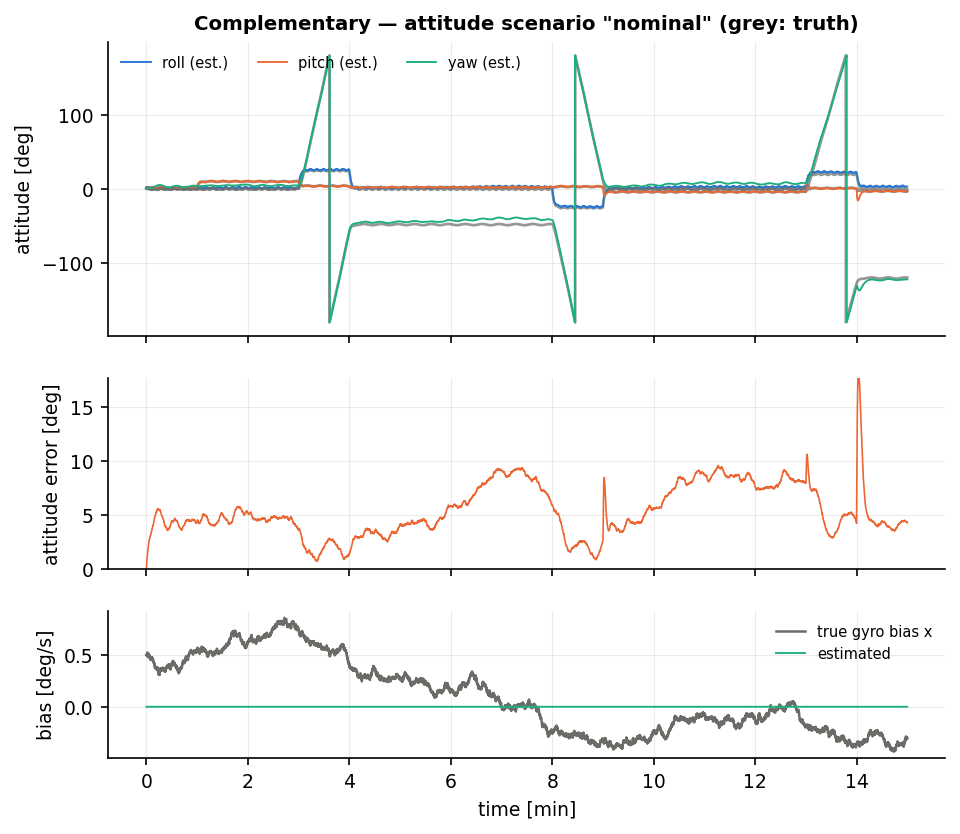
\includegraphics[width=\textwidth]{figures/imu_Complementary_nominal.png}
\caption{Complementary filter on the nominal mission: true and estimated Euler angles (top), total
angular error (middle), gyro-bias channel (bottom).}
\end{figure}
\begin{figure}[H]\centering
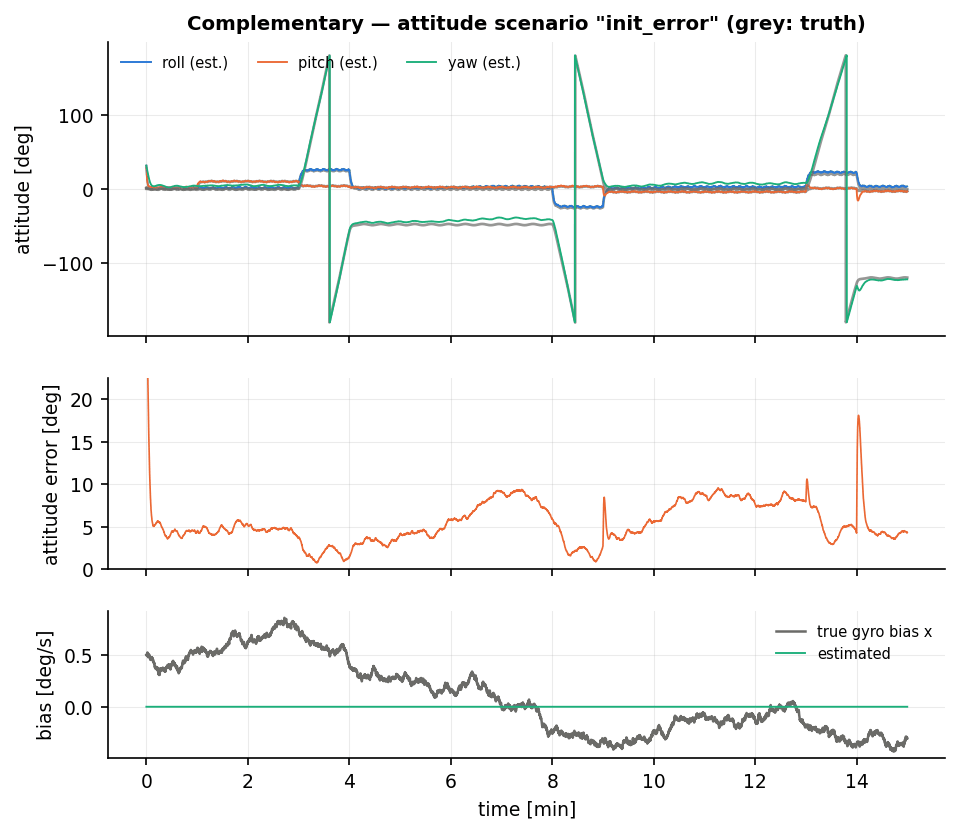
\includegraphics[width=\textwidth]{figures/imu_Complementary_init_error.png}
\caption{Complementary filter with a $30^\circ$ initial error on each Euler axis ($46.6^\circ$ of
total attitude error).}
\end{figure}
\begin{figure}[H]\centering
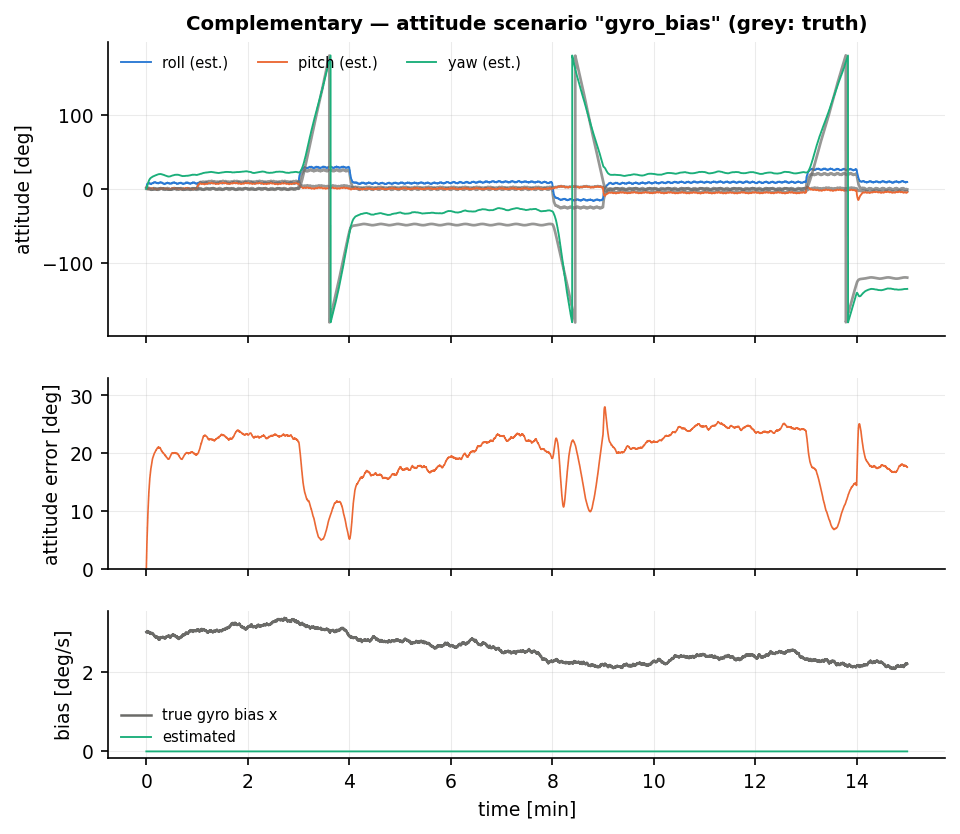
\includegraphics[width=\textwidth]{figures/imu_Complementary_gyro_bias.png}
\caption{Complementary filter on \texttt{gyro\_bias} ($\SI{3}{\degree\per\second}$ per axis): with
no bias state the centripetal correction \eqref{eq:cf-centri} multiplies the rate error by
$V/g\approx4.6$, and the tilt error it produces is amplified again into heading by the
$65^\circ$ magnetic dip.}
\end{figure}

On \texttt{nominal} the filter reaches $\text{RMS}=\SI{6.57}{\degree}$ (roll $2.78$, pitch $1.18$,
yaw $\SI{5.80}{\degree}$), $\text{RMS}_{\text{ss}}=\SI{7.91}{\degree}$, peak $\SI{17.5}{\degree}$, at
$\SI{362}{\nano\second}$/step and 272\,bytes. It passes the convergence test at
$t=\SI{37}{\second}$ --- the reduction of the dataset's residual hard iron to
$\SI{0.42}{\micro\tesla}$ brought its error briefly below $2^\circ$ --- and it is never marked
lost, on any scenario. Its \emph{bias} RMSE column simply reproduces the true bias magnitude
($1.03$ and $\SI{3.80}{\degree\per\second}$), because the filter has no bias state and reports zero.

Numbers quoted from the table are three-seed means; the ablations below are single-seed (seed~1)
diagnostics and are internally consistent with each other, not with the table to the last digit.

\paragraph{The centripetal correction is worth a factor of three.} Measured on \texttt{nominal}
with $\tau_a=\SI{1}{\second}$: $V=0$ (no correction) gives $\SI{18.36}{\degree}$, $V=20$ gives
$9.92$, $V=30$ gives $6.87$, $V=45$ (registered, the true cruise airspeed) gives $5.89$, and
$V=60$ gives $\SI{9.56}{\degree}$. The optimum sits at the true airspeed and the penalty for a
$\pm33\,\%$ airspeed error is $3$--$\SI{4}{\degree}$: the correction is useful but not forgiving.
Per flight phase (registered configuration, seed~1) the error is
\[
4.26\;/\;4.71\;/\;2.01\;/\;6.24\;/\;3.34\;/\;7.40\;/\;6.91\;/\;5.02\ \SI{}{\degree}
\]
for take-off / climb / turn\,1 / cruise / turn\,2 / descent / turn\,3 / final: \emph{with} the
correction the turns are among the \emph{best} phases, not the worst. Without it the turn phases are
$40$--$\SI{45}{\degree}$, exactly like the memory-less estimators of Chapters~\ref{ch:att-triad}
and~\ref{ch:att-quest}.

\paragraph{The gyro bias is the price.} On \texttt{gyro\_bias} ($\SI{3}{\degree\per\second}$ per
axis) the RMS rises to $\SI{17.58}{\degree}$, while the same filter with $V=0$ gives
$\SI{19.22}{\degree}$ --- i.e. the correction has almost stopped helping.
Equation~\eqref{eq:cf-amplify} predicts the size: the $y$ and $z$ bias components of $1.8$ and
$\SI{1.2}{\degree\per\second}$ give $V\delta\omega=1.41$ and
$\SI{0.94}{\metre\per\second\squared}$, i.e. $8.2^\circ$ and $5.5^\circ$ of tilt error, and the
measured roll RMS is $\SI{7.41}{\degree}$. The magnetic-dip amplification discussed below then
turns that into $\SI{15.89}{\degree}$ of heading error. This is the cleanest demonstration in the
family of why the bias must be a state: the six-state filters of Chapters~\ref{ch:att-mekf}
and~\ref{ch:att-iekf} are unaffected by this scenario ($\SI{2.48}{\degree}$, unchanged from
nominal).

\paragraph{Tuning sensitivity.} With the correction on, $\tau_a=0.5/1/\SI{2}{\second}$ give
$5.59/5.89/\SI{6.68}{\degree}$ on \texttt{nominal} and $16.4/20.1/\SI{27.8}{\degree}$ on
\texttt{gyro\_bias}, the latter following \eqref{eq:cf-bias} almost exactly. Without the correction
the ordering reverses on \texttt{nominal} ($19.0/18.4/16.9$), because a slower filter rejects more
of the manoeuvre disturbance. $\SI{1}{\second}$ is the compromise, and it is inside the range the
assignment prescribes.

\paragraph{Disturbance scenarios.} \texttt{mag\_disturbance} (a $\SI{25}{\micro\tesla}$ offset for
$\SI{20}{\second}$ at $t=\SI{300}{\second}$) costs $\SI{0.14}{\degree}$ of mission RMS
($6.71$ against $6.57$), because the magnitude gate sees $\norm{\bm{m}}$ rise from $48$ to
$\SI{54}{\micro\tesla}$ and switches the heading branch off; with the gate disabled the same
scenario costs $\SI{3.2}{\degree}$ ($9.12$ against $\SI{5.87}{\degree}$, seed~1).
\texttt{vibration} ($\sigma_a=\SI{1.05}{\metre\per\second\squared}$) is free ($6.58$): the
$\SI{1}{\second}$ low-pass attenuates broadband accelerometer noise by
$\sqrt{\dt/2\tau_a}=0.07$. \texttt{high\_dynamics} is free as well ($6.58$).
\texttt{init\_error} costs $\SI{0.2}{\degree}$ of mission RMS but takes $\SI{17.9}{\second}$ to
bring a $46.6^\circ$ error below $5^\circ$ --- the price of a fixed first-order low-pass whose tilt
and heading loops have to unwind sequentially.

\paragraph{Where the residual $\SI{5.8}{\degree}$ of yaw comes from.} After the recalibration of the
simulated compass this is now \emph{almost entirely} dip-amplified tilt error, and the hard iron is
a minor term. The dataset's residual hard-iron offset is
$\bm{b}_m=[0.30,-0.15,0.25]^\T\,\SI{}{\micro\tesla}$, $\norm{\bm{b}_m}=\SI{0.42}{\micro\tesla}$ or
$0.87\,\%$ of the field; fed to an \emph{exact} tilt-compensated compass it alone produces only
$\SI{0.65}{\degree}$ RMS ($\SI{1.12}{\degree}$ peak) of heading error. The dominant term is the
leakage of tilt error into the tilt-compensated heading with gain $\tan I = 2.14$ at $I=65^\circ$:
the residual roll RMS of $\SI{2.78}{\degree}$ --- itself the $V/g$-amplified gyro-bias random walk
of \eqref{eq:cf-amplify} --- contributes $2.78\times2.14\approx\SI{5.9}{\degree}$, which together
with $\SI{0.65}{\degree}$ of hard iron accounts for the measured $\SI{5.80}{\degree}$. Reducing the
tilt error, not the magnetometer error, is what would improve this filter.

\section{Summary}
Use the complementary filter when the platform is calibrated, the noise statistics are stationary
and the code budget is a few hundred bytes: it costs one quaternion, has one knob per channel, and
its steady-state error is the closed-form $b\tau$ of \eqref{eq:cf-bias}. On a fixed-wing aircraft
it is unusable without the Euston centripetal correction --- $18.4^\circ$ versus $\SI{6.6}{\degree}$
RMS here --- and the correction in turn amplifies gyro-bias error by $V/g\approx4.6$, which is why
this filter is $\SI{17.6}{\degree}$ on \texttt{gyro\_bias} where the six-state filters of
Chapters~\ref{ch:att-mekf} and \ref{ch:att-iekf} are $\SI{2.5}{\degree}$. Do not use it when the
gyro bias is unknown, when the disturbance statistics change during the mission, or when a
covariance is needed downstream.

% Copyright 2026 Sreeram Anil
% SPDX-License-Identifier: CC-BY-4.0
% =============================================================================
%  Madgwick gradient-descent MARG filter — attitude (AHRS) family
% =============================================================================
\chapter{Gradient-Descent MARG Filter (Madgwick)}
\label{ch:att-madgwick}

\section*{At a glance}
\begin{tabular}{@{}l>{\raggedright\arraybackslash}p{0.76\textwidth}@{}}
Family & attitude / AHRS \\
Header & \texttt{include/estkit/attitude/madgwick.hpp} \\
Registered names & \texttt{Madgwick} (published), \texttt{Madgwick-Gated} (practical variant) \\
State & unit quaternion $\bm{q}\in S^3$ and gyro bias $\bm{b}\in\real^3$ (7 reals) \\
Cost per step & $\approx300$ flops, one \code{sqrt};
  $112$ / $\SI{138}{\nano\second}$ per step, 272\,bytes \\
Tuning & $\beta=0.1\,\SI{}{\radian\per\second}$, $\zeta=0$ (published defaults) \\
Primary references & \cite{madgwick2011,madgwick2010} \\
\end{tabular}

\section{Motivation and aerospace relevance}
Madgwick's filter is the cheapest MARG algorithm in wide use: no matrix, no covariance, one
normalisation and one tuning constant. It became the de-facto standard for small UAV autopilots,
motion capture and rehabilitation robotics precisely because it fits in a few hundred bytes on an
8-bit micro-controller and still fuses nine axes correctly.

Its conceptual contribution is to pose the vector-observation problem as an \emph{optimisation} and
then take exactly one normalised gradient step per sample. The gyro supplies the prediction; the
gradient step supplies a correction whose \emph{direction} is optimal in the least-squares sense and
whose \emph{magnitude} is a constant $\beta$. Choosing a constant magnitude rather than a
covariance-weighted one is what makes the filter cheap, and --- as this benchmark shows --- also
what makes it insensitive to the size of the disturbance it is fighting.

The second contribution is the magnetic-distortion compensation of
\cite[Sec.~3.3]{madgwick2010}: instead of a tabulated field vector, the reference is rebuilt each
step from the measurement itself, constrained to lie in the vertical plane containing magnetic
north. Any error in the assumed declination, and any horizontal distortion, is then confined to the
heading channel and cannot tilt the horizon. That trick is worth having in any MARG filter.

\section{Problem statement and assumptions}
Conventions as in Chapter~\ref{ch:att-complementary}: $\bm{q}$ maps BODY(FRD) to NAV(NED),
$\bm{R}(\bm{q})$ is its rotation matrix, the gyro measures $\bm{\omega}_y=\bm{\omega}+\bm{b}+\bm{n}_v$,
and the normalised specific force at rest equals $\bm{R}^\T\bm{d}_a$ with $\bm{d}_a=[0,0,-1]^\T$.

The filter assumes that the accelerometer measures gravity and that the magnetometer measures the
local field, with \emph{unknown but bounded} errors of total size $\omega_\beta$ expressed as an
equivalent gyro-rate error; $\beta=\sqrt{3/4}\,\omega_\beta$ is the resulting gain
\cite[Sec.~3.5]{madgwick2010}. It makes no distributional assumption and carries no uncertainty.

\subsection*{Frame mapping to this dataset}
Madgwick's published equations use a gravity reference $\bm{d}=[0,0,1]^\T$ together with an
accelerometer that reads $+1\,g$ on the vertical axis at rest (the ``reaction force'' convention in
a $z$-up earth frame). This benchmark is NED/FRD with the specific-force convention
$\bm{f}=\bm{a}-\bm{g}$, so a level accelerometer reads $[0,0,-g]^\T$ and the NAV reference of the
normalised accelerometer is
\begin{equation}
\bm{d}_a = [0,0,-1]^\T .
\label{eq:mw-da}
\end{equation}
Since the objective $\bm{f}_i$ and its Jacobian $\bm{J}_i$ defined below are both \emph{linear} in
$\bm{d}$, replacing $\bm{d}$ by $-\bm{d}$ changes the sign of both, and the gradient
$\bm{J}^\T\bm{f}$ is unchanged. This implementation is therefore bit-for-bit Madgwick's algorithm
applied to the negated accelerometer. The quaternion convention needs no change at all: Madgwick's
reference code propagates $\dot{\bm{q}}=\tfrac12\bm{q}\otimes[0,\bm{\omega}]$ with $\bm{\omega}$ in
the sensor frame and evaluates $\bm{R}(\bm{q})^\T\bm{d}$, which is exactly the BODY$\to$NAV Hamilton
quaternion used here. The magnetic part transfers verbatim because it uses the measured vertical
component whatever its sign (here $h_3>0$: the field dips downwards and NED $z$ points down).

\section{Derivation}

\subsection{The objective and its gradient}
Let $\bm{d}\in\real^3$ be a known NAV direction and $\bm{s}\in\real^3$ the corresponding measured
BODY direction, both unit. The orientation is correct when
\begin{equation}
\bm{f}(\bm{q};\bm{d},\bm{s}) \;=\; \bm{R}(\bm{q})^\T\bm{d}-\bm{s} \;=\; \bm{0}\in\real^3 ,
\label{eq:mw-f}
\end{equation}
an under-determined system (three equations, one unobservable rotation about $\bm{d}$) whose
least-squares solution is sought by steepest descent on
$F(\bm{q})=\tfrac12\norm{\bm{f}}^2$. With $\bm{q}=[q_w,q_x,q_y,q_z]$ the components of
\eqref{eq:mw-f} are
\begin{align}
f_1 &= d_1(1-2q_y^2-2q_z^2) + d_2(2q_xq_y+2q_wq_z) + d_3(2q_xq_z-2q_wq_y) - s_1,\nonumber\\
f_2 &= d_1(2q_xq_y-2q_wq_z) + d_2(1-2q_x^2-2q_z^2) + d_3(2q_yq_z+2q_wq_x) - s_2,\label{eq:mw-fexp}\\
f_3 &= d_1(2q_xq_z+2q_wq_y) + d_2(2q_yq_z-2q_wq_x) + d_3(1-2q_x^2-2q_y^2) - s_3,\nonumber
\end{align}
and the Jacobian $\bm{J}=\partial\bm{f}/\partial\bm{q}\in\real^{3\times4}$ is
\begin{equation}
\bm{J} = 2\!\begin{bmatrix}
 d_2q_z-d_3q_y & d_2q_y+d_3q_z & d_2q_x-d_3q_w-2d_1q_y & d_2q_w+d_3q_x-2d_1q_z\\
 d_3q_x-d_1q_z & d_1q_y+d_3q_w-2d_2q_x & d_1q_x+d_3q_z & d_3q_y-d_1q_w-2d_2q_z\\
 d_1q_y-d_2q_x & d_1q_z-d_2q_w-2d_3q_x & d_1q_w+d_2q_z-2d_3q_y & d_1q_x+d_2q_y
\end{bmatrix}.
\label{eq:mw-J}
\end{equation}
Substituting $\bm{d}=[0,0,1]^\T$ into \eqref{eq:mw-fexp}--\eqref{eq:mw-J} reproduces Madgwick's
Eqs.~(25)--(26) exactly; substituting \eqref{eq:mw-da} reproduces them with both signs flipped, as
argued above. With $m$ observations stacked,
\begin{equation}
\nabla F(\bm{q}) = \sum_{i=1}^{m}\bm{J}_i^\T\bm{f}_i \in\real^4,
\qquad
\dot{\bm{q}}_\varepsilon = \frac{\nabla F}{\norm{\nabla F}} .
\label{eq:mw-grad}
\end{equation}
The normalisation in \eqref{eq:mw-grad} is the crux of the method: the descent \emph{direction} is
computed from the data, the descent \emph{step} is the constant $\beta$. Madgwick's argument is
that the convergence rate of the estimate must merely exceed the divergence rate of the gyro
integration, and that the latter is bounded by $\omega_\beta$; a step proportional to the residual
would be faster when the residual is large, which is exactly when the residual is least likely to be
trustworthy.

\subsection{Fusion and the filter equations}
The two rates are combined and integrated with a single explicit Euler step:
\begin{align}
\dot{\bm{q}}_\omega &= \tfrac12\,\bm{q}\otimes[0,\bm{\omega}_c],\qquad \bm{\omega}_c=\bm{\omega}_y-\bm{b},\label{eq:mw-qw}\\
\dot{\bm{q}} &= \dot{\bm{q}}_\omega - \beta\,\dot{\bm{q}}_\varepsilon,\label{eq:mw-qdot}\\
\bm{q}_{k+1} &= \frac{\bm{q}_k+\dot{\bm{q}}\,\dt}{\norm{\bm{q}_k+\dot{\bm{q}}\,\dt}} .\label{eq:mw-int}
\end{align}
Equations \eqref{eq:mw-qw}--\eqref{eq:mw-int} are Madgwick's (42)--(44).

\subsection{Magnetic-distortion compensation (Sec.~3.3)}
Rather than a stored $\bm{m}_{\text{nav}}$, the reference is rebuilt each step from the measurement
by rotating it into the navigation frame and flattening its horizontal part onto north:
\begin{equation}
\bm{h} = \bm{R}(\bm{q})\,\hat{\bm{m}},\qquad
\bm{d}_m = \big[\sqrt{h_1^2+h_2^2},\;0,\;h_3\big]^\T .
\label{eq:mw-flux}
\end{equation}
By construction $\bm{d}_m$ has no east component, so the objective can never ask the filter to
change its \emph{inclination} estimate: an erroneous declination or a horizontal distortion is
absorbed entirely by the heading. The price is that the magnetometer no longer carries any
independent information about the dip angle, and therefore contributes less to roll and pitch than
a known reference would.

\subsection{Gyro-bias drift compensation (Sec.~3.4)}
The normalised gradient is a quaternion rate, so the body rate that would produce it is
\begin{equation}
\bm{\omega}_\varepsilon = 2\,\bm{q}^*\otimes\dot{\bm{q}}_\varepsilon
\quad(\text{vector part}),
\label{eq:mw-werr}
\end{equation}
which points along the axis about which the estimate is currently being corrected, i.e. along the
rate error that created the misalignment. Integrating it with gain $\zeta$ gives a bias estimate and
a corrected rate,
\begin{equation}
\bm{b}_{k+1}=\bm{b}_k+\zeta\,\bm{\omega}_\varepsilon\,\dt,
\qquad \bm{\omega}_c = \bm{\omega}_y-\bm{b} .
\label{eq:mw-bias}
\end{equation}
$\zeta$ has units of angular acceleration; Madgwick recommends $\zeta=\sqrt{3/4}\,\dot\omega_\beta$
with $\dot\omega_\beta$ the gyro bias drift rate. Because $\norm{\dot{\bm{q}}_\varepsilon}=1$ by
construction, $\norm{\bm{\omega}_\varepsilon}=2$ always: \eqref{eq:mw-bias} is a \emph{sign-like}
integrator that slews at a constant $2\zeta\,\SI{}{\radian\per\second\squared}$ regardless of how
large the bias error is. That makes it robust but also means it never settles --- it dithers about
the true bias with amplitude $2\zeta\dt$ per step.

\begin{remark}[Why $\zeta=0$ in the plain \texttt{Madgwick} instance]
The bias loop \eqref{eq:mw-bias} is driven by the same gradient that the manoeuvre disturbance
drives. On a fixed-wing mission with sustained coordinated turns, $\bm{\omega}_\varepsilon$ has a
long-lived non-zero mean during each turn, and the integrator walks: the measured bias RMSE on
\texttt{nominal} rises monotonically from $\SI{0.62}{\degree\per\second}$ (no estimate at all, i.e.
the true bias magnitude) at $\zeta=0$ to $1.00$, $1.50$ and $\SI{2.40}{\degree\per\second}$ at
$\zeta=0.005$, $0.01$ and $0.03$, and the attitude RMS rises with it. \emph{On its own}, $\zeta$ is
harmful; it is useful only together with disturbance rejection, which is why the two are enabled
together in the second registered instance (\S\ref{sec:mw-gated}) and neither is enabled in the
first. $\zeta=0$ also makes the plain instance identical to \code{ahrs.filters.Madgwick}: the
integrator's cross-validation measures a maximum angular difference of $0.0014^\circ$ over the
$9\times10^4$ samples of the nominal flight (Table~\ref{tab:val_ahrs}).
\end{remark}

\section{Algorithm}
\begin{algorithm}[H]
\caption{Madgwick MARG --- one sampling period}
\begin{algorithmic}[1]
\Require $\bm{q}_{k-1},\bm{b}_{k-1},\bm{\omega}_y,\bm{f},\bm{m}$; $\beta,\zeta$
\State $\hat{\bm{a}}\gets\bm{f}/\norm{\bm{f}}$, \; $\hat{\bm{m}}\gets\bm{m}/\norm{\bm{m}}$
\State $\nabla F \gets \bm{J}^\T(\bm{q},\bm{d}_a,\hat{\bm{a}})\,\bm{f}(\bm{q},\bm{d}_a,\hat{\bm{a}})$
       \Comment{$\bm{d}_a=[0,0,-1]^\T$, \eqref{eq:mw-da}}
\State $\bm{h}\gets\bm{R}(\bm{q})\hat{\bm{m}}$;\; $\bm{d}_m\gets[\sqrt{h_1^2+h_2^2},0,h_3]^\T$
       \Comment{flux compensation, \eqref{eq:mw-flux}}
\State $\nabla F \mathrel{+}= \bm{J}^\T(\bm{q},\bm{d}_m,\hat{\bm{m}})\,\bm{f}(\bm{q},\bm{d}_m,\hat{\bm{m}})$
\State $\dot{\bm{q}}_\varepsilon\gets\nabla F/\norm{\nabla F}$
\If{$\zeta>0$} \Comment{Sec.~3.4}
  \State $\bm{\omega}_\varepsilon\gets\operatorname{vec}(2\,\bm{q}^*\otimes\dot{\bm{q}}_\varepsilon)$;\;
         $\bm{b}\gets\operatorname{clamp}(\bm{b}+\zeta\bm{\omega}_\varepsilon\dt)$
\EndIf
\State $\dot{\bm{q}}\gets\tfrac12\bm{q}\otimes[0,\bm{\omega}_y-\bm{b}]-\beta\dot{\bm{q}}_\varepsilon$
\State $\bm{q}_k\gets(\bm{q}+\dot{\bm{q}}\dt)/\norm{\bm{q}+\dot{\bm{q}}\dt}$
\Ensure $\bm{q}_k,\bm{b}_k$
\end{algorithmic}
\end{algorithm}

\section{Application to the benchmark flight}
$\beta=0.1\,\SI{}{\radian\per\second}$ is the value the assignment prescribes and sits at the top of
Madgwick's recommended band: $\beta=\sqrt{3/4}\,\omega_\beta$ gives
$\omega_\beta=\SI{6.6}{\degree\per\second}$ of assumed gyro error, which is generous for the
$\SI{0.1}{\degree\per\second}$ noise and $\SI{0.5}{\degree\per\second}$ bias of the nominal
scenario. $\zeta=0$ and no manoeuvre gating: the \texttt{Madgwick} instance is the published algorithm,
nothing added. The \code{gate} switch in \code{Options} weights the two objectives in
\eqref{eq:mw-grad} by the disturbance weight \eqref{eq:cf-weight} of
Chapter~\ref{ch:att-complementary}; together with $\zeta=0.005$ it forms the second registered
instance, \texttt{Madgwick-Gated}, documented in \S\ref{sec:mw-gated}.

\section{Implementation notes}
The whole step is two evaluations of \eqref{eq:mw-fexp}--\eqref{eq:mw-J} (24 multiply--adds each
for $\bm{J}^\T\bm{f}$, plus about 40 for the entries), one 4-vector normalisation, one quaternion
product and one 4-vector normalisation: about 300 flops and a single \code{sqrt} beyond the two
measurement normalisations. Measured: $\SI{112}{\nano\second}$/step for the plain instance and
$\SI{138}{\nano\second}$ with the gate, the cheapest filter in the family that uses the gyro;
\code{sizeof} is 272\,bytes, of which $7\times8$ are the state. On a $\SI{216}{\mega\hertz}$
Cortex-M7 in float32 this is of order $\SI{2}{\micro\second}$/step, $0.02\,\%$ of the
$\SI{10}{\milli\second}$ budget at $\SI{100}{\hertz}$.

Guards: the accelerometer and magnetometer branches are skipped if the corresponding magnitude is
below $10^{-6}$; the gradient step is skipped if $\norm{\nabla F}<10^{-12}$, in which case the
filter degenerates gracefully to pure gyro integration; the quaternion is renormalised every step,
which is the only thing that keeps the explicit Euler integration \eqref{eq:mw-int} on the sphere;
the bias state is clamped to $\pm\SI{10}{\degree\per\second}$. The single-precision build reproduces
the double-precision mission RMS to five digits on \texttt{nominal}.

Two structural limitations are worth stating. First, \eqref{eq:mw-int} is an explicit Euler step:
the local truncation error is $O(\dt^2\norm{\ddot{\bm{q}}})$ and the renormalisation hides it, but at
low sample rates or high rates of turn it shows up as a lag. Second, there is no covariance, so the
filter cannot trade roll accuracy against heading accuracy, and it cannot tell a large residual
caused by a large attitude error from one caused by a large disturbance --- the correction is
$\beta$ either way.

\section{Benchmark results}
% Copyright 2026 Sreeram Anil
% SPDX-License-Identifier: CC-BY-4.0
\begin{table}[H]\centering\footnotesize\setlength{\tabcolsep}{3.5pt}\caption{Madgwick: attitude benchmark (mean over seeds; all angles in degrees; $t_\mathrm{conv}$: first time the attitude error stays below 2$^\circ$ for 30\,s; bias RMSE in deg/s; 272 bytes of state).}\label{tab:imu_Madgwick}
\begin{tabular}{lrrrrrrrrcr}\toprule scenario & RMS & roll & pitch & yaw & max & RMS$_\mathrm{ss}$ & $t_\mathrm{conv}$ [s] & bias RMSE & lost & ns/step \\ \midrule
nominal & 17.60 & 9.06 & 1.28 & 15.28 & 71.4 & 18.96 & -- & 1.03 & yes & 112 \\
init\_error & 17.74 & 9.14 & 1.73 & 15.37 & 71.4 & 18.96 & -- & 1.03 & yes & 112 \\
gyro\_bias & 17.62 & 9.01 & 1.29 & 15.33 & 69.4 & 19.41 & 281 & 3.80 & yes & 111 \\
mag\_disturbance & 19.01 & 9.06 & 1.48 & 16.87 & 71.4 & 18.96 & -- & 1.03 & yes & 109 \\
vibration & 14.78 & 8.40 & 1.76 & 12.27 & 50.9 & 16.53 & -- & 1.03 & yes & 112 \\
high\_dynamics & 18.43 & 9.41 & 1.42 & 16.04 & 81.8 & 19.58 & -- & 1.03 & yes & 111 \\
\bottomrule\end{tabular}\end{table}

\begin{figure}[H]\centering
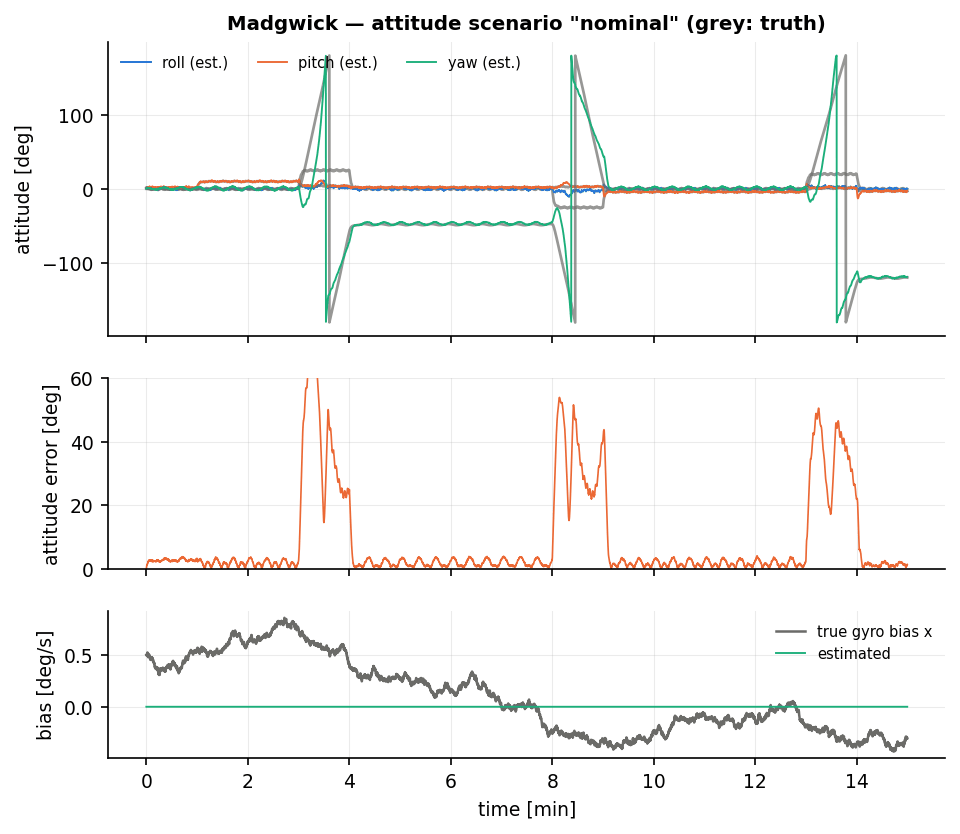
\includegraphics[width=\textwidth]{figures/imu_Madgwick_nominal.png}
\caption{Madgwick (published, $\beta=0.1$, $\zeta=0$) on the nominal mission: the three
$\SI{60}{\second}$ coordinated turns dominate the error budget.}
\end{figure}
\begin{figure}[H]\centering
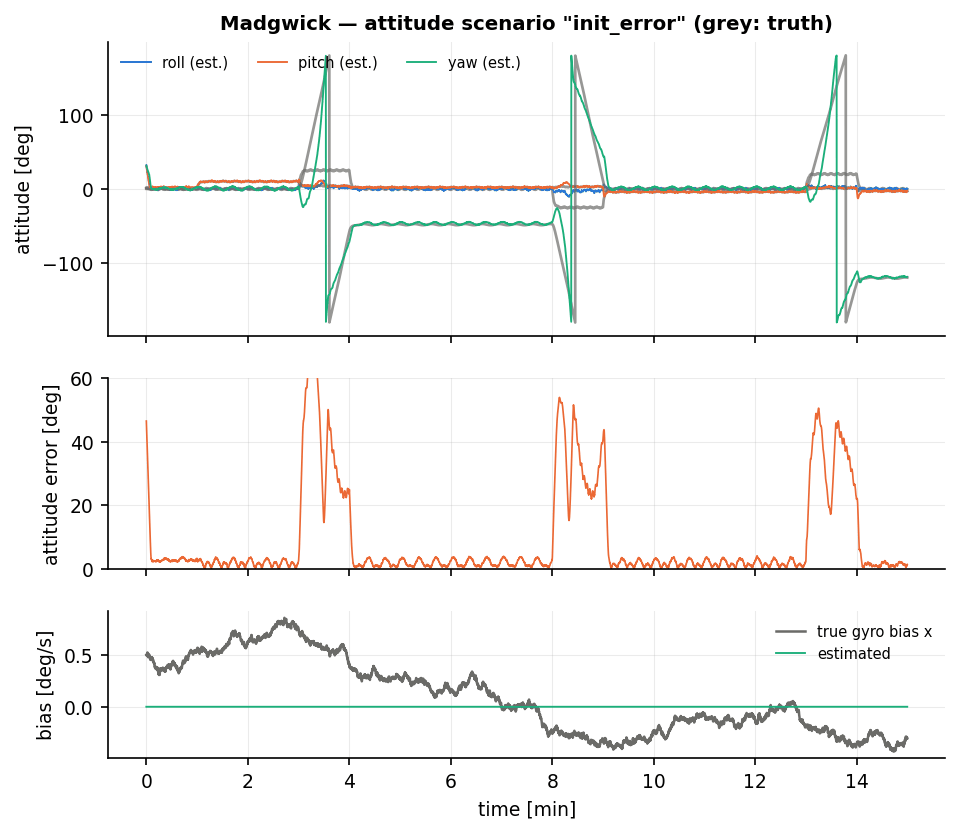
\includegraphics[width=\textwidth]{figures/imu_Madgwick_init_error.png}
\caption{Madgwick filter with a $46.6^\circ$ initial attitude error; the convergence rate is
limited by $\beta$, not by the size of the error.}
\end{figure}

On \texttt{nominal} the published filter gives $\text{RMS}=\SI{17.60}{\degree}$
(roll $9.06$, pitch $1.28$, yaw $\SI{15.28}{\degree}$), $\text{RMS}_{\text{ss}}=\SI{18.96}{\degree}$,
peak $\SI{71.4}{\degree}$, $\SI{112}{\nano\second}$/step, 272\,bytes, and is marked \emph{lost} on
every scenario but none. The per-phase breakdown (seed~1) explains the whole number at once:
\[
\underbrace{2.77}_{\text{take-off}}\;
\underbrace{2.07}_{\text{climb}}\;
\underbrace{\mathbf{42.05}}_{\text{turn 1}}\;
\underbrace{2.14}_{\text{cruise}}\;
\underbrace{\mathbf{35.52}}_{\text{turn 2}}\;
\underbrace{2.15}_{\text{descent}}\;
\underbrace{\mathbf{34.80}}_{\text{turn 3}}\;
\underbrace{1.53}_{\text{final}}\ \SI{}{\degree}.
\]
In level flight the filter is a $\SI{1.5}{\degree}$--$\SI{2.8}{\degree}$ device, i.e. within a
factor of two of the $\SI{0.65}{\degree}$ hard-iron floor of this dataset; during the three
$\SI{60}{\second}$ coordinated turns it is a $\SI{35}{\degree}$--$\SI{42}{\degree}$ device. The
mechanism is the one analysed in Chapter~\ref{ch:att-complementary}: in a coordinated turn the
accelerometer reports zero bank, and $\beta$ is a \emph{fixed} correction magnitude, so the filter
converges to the accelerometer's answer at the same rate whether that answer is right or wrong. The
$23^\circ$ tilt error is then amplified into $\approx\!50^\circ$ of heading error by the
$\tan I=2.14$ dip factor, which is why the yaw RMS ($15.28$) is larger than the roll RMS ($9.06$).

Table numbers are three-seed means; the sweeps below are single-seed (seed~1) diagnostics.

\paragraph{$\beta$ sensitivity.} On \texttt{nominal}:
$\beta=0.01\to13.95$, $0.033\to12.70$, $0.05\to15.41$, $0.1\to17.60$, $0.2\to18.68$,
$0.3\to\SI{18.99}{\degree}$. Smaller $\beta$ is better here for the obvious reason --- it slows the
filter's approach to the wrong accelerometer answer during the turns --- but it is not free:
$\beta=0.01$ costs $\SI{108.6}{\degree}$ on \texttt{gyro\_bias} (the correction can no longer keep
up with a $\SI{3}{\degree\per\second}$ drift, since $\beta$ must exceed the drift rate) and
$\SI{46.6}{\degree}$ on \texttt{vibration}. $\beta=0.033$ --- the bottom of the assignment's band ---
is the best compromise at $12.70/13.28/22.48/14.00/12.70/\SI{12.49}{\degree}$ across the six
scenarios, against $17.60/17.74/17.70/18.99/14.03/\SI{18.39}{\degree}$ for the registered
$\beta=0.1$. The registered value was kept because the assignment prescribes it and because
$\beta=0.1$ is the value most implementations ship.

\paragraph{$\zeta$ sensitivity.} At $\beta=0.1$ without gating,
\[
\zeta = 0\;/\;0.002\;/\;0.005\;/\;0.01\;/\;0.03
\ \Longrightarrow\
17.60\;/\;18.15\;/\;18.98\;/\;20.09\;/\;25.48\ \SI{}{\degree}
\]
with bias RMSE $0.62$, $0.63$, $1.00$, $1.50$ and $\SI{2.40}{\degree\per\second}$: the bias
integrator on its own is monotonically harmful, for the reason given in the remark above.

\paragraph{Other scenarios.} \texttt{vibration} is the only scenario on which the published filter
does \emph{better} than nominal ($14.78$ versus $\SI{17.60}{\degree}$): the added
$\SI{1}{\metre\per\second\squared}$ of broadband accelerometer noise perturbs the gradient
\emph{direction} but not its magnitude, and the constant-$\beta$ step averages it out --- an
accidental benefit of not being covariance-weighted. \texttt{mag\_disturbance} costs
$\SI{1.4}{\degree}$ ($19.01$); the flux compensation \eqref{eq:mw-flux} confines the
$\SI{25}{\micro\tesla}$ offset to the heading, as designed. \texttt{gyro\_bias} costs almost nothing
($17.62$) because $\beta\gg$ the bias: the correction bandwidth is set by $\beta$, not by the
disturbance --- and, oddly, it is the only scenario on which the plain filter passes the convergence
test ($t_{\text{conv}}=\SI{281}{\second}$), because a large bias briefly biases the estimate
\emph{towards} truth during one of the turns. Turning the magnetometer off
(\code{use\_mag=false}) gives $\SI{87.4}{\degree}$, confirming that heading is unobservable from
gravity alone.

\paragraph{Initial-error transient.} Starting from $46.6^\circ$ of attitude error the filter needs
$\SI{5.3}{\second}$ to reach $5^\circ$; from $78.5^\circ$, $\SI{9.5}{\second}$; from $90^\circ$,
$\SI{10.3}{\second}$. The slope is $\approx\SI{7.9}{\degree\per\second}$ and is independent of the
error, as \eqref{eq:mw-qdot} requires (the body-rate magnitude of the correction is at most
$2\beta=\SI{11.5}{\degree\per\second}$). Compare the MEKF's $\SI{0.17}{\second}$ and the invariant
EKF's $\SI{0.01}{\second}$ from the same $46.6^\circ$: a covariance-weighted filter knows that the
residual is large because the \emph{state} is wrong, and takes a correspondingly large step.

\section{The gated variant (\texttt{Madgwick-Gated})}\label{sec:mw-gated}
The second registered instance switches on both of the mechanisms that the published algorithm
leaves out, and it is important to be explicit that this is an \textbf{engineering addition, not
part of Madgwick's method}: the objectives in \eqref{eq:mw-grad} are weighted by the disturbance
weight \eqref{eq:cf-weight} of Chapter~\ref{ch:att-complementary} (magnitude anomaly plus the
rate-driven manoeuvre bound of Chapter~\ref{ch:att-mekf}, Remark~\ref{rem:mekf-turn}), and the
bias-drift compensation of Sec.~3.4 is enabled with $\zeta=0.005$. Everything else --- $\beta=0.1$,
the gradient \eqref{eq:mw-grad}, the flux compensation \eqref{eq:mw-flux}, the explicit Euler step
\eqref{eq:mw-int} --- is unchanged, and the cost rises only from $112$ to
$\SI{138}{\nano\second}$/step at the same 272\,bytes.

\begin{remark}[The gate and the bias state are a package deal]\label{rem:mw-package}
The manoeuvre detector needs an angular rate that is free of bias, because it declares a manoeuvre
whenever $V_{\text{ref}}\norm{\bm{\omega}_{yz}}$ exceeds a threshold. With $\zeta=0$ there is no
bias estimate, so on \texttt{gyro\_bias} the $\SI{3}{\degree\per\second}$ offset looks like a
permanent turn, the accelerometer is latched off for the whole mission, and only the magnetometer
remains: measured $\SI{55.3}{\degree}$ RMS, against $\SI{10.1}{\degree}$ on nominal. Conversely
$\zeta>0$ without the gate walks, as shown above. Enabling both gives
$\SI{4.81}{\degree}$ on \texttt{nominal} and $\SI{4.81}{\degree}$ on \texttt{gyro\_bias} (seed~1) ---
the two mechanisms fix each other's failure mode, and either one alone is worse than neither.
\end{remark}

% Copyright 2026 Sreeram Anil
% SPDX-License-Identifier: CC-BY-4.0
\begin{table}[H]\centering\footnotesize\setlength{\tabcolsep}{3.5pt}\caption{Madgwick-Gated: attitude benchmark (mean over seeds; all angles in degrees; $t_\mathrm{conv}$: first time the attitude error stays below 2$^\circ$ for 30\,s; bias RMSE in deg/s; 272 bytes of state).}\label{tab:imu_MadgwickGated}
\begin{tabular}{lrrrrrrrrcr}\toprule scenario & RMS & roll & pitch & yaw & max & RMS$_\mathrm{ss}$ & $t_\mathrm{conv}$ [s] & bias RMSE & lost & ns/step \\ \midrule
nominal & 5.78 & 2.48 & 2.46 & 4.60 & 22.8 & 7.43 & -- & 0.22 & no & 138 \\
init\_error & 6.17 & 2.75 & 2.72 & 4.88 & 46.5 & 7.43 & -- & 0.30 & no & 140 \\
gyro\_bias & 5.79 & 2.48 & 2.46 & 4.60 & 22.8 & 7.43 & -- & 0.44 & no & 138 \\
mag\_disturbance & 5.78 & 2.48 & 2.46 & 4.59 & 22.8 & 7.43 & -- & 0.22 & no & 136 \\
vibration & 3.22 & 1.67 & 1.78 & 2.08 & 12.5 & 3.52 & 263 & 0.17 & no & 138 \\
high\_dynamics & 5.34 & 2.78 & 2.58 & 3.76 & 16.6 & 6.20 & -- & 0.24 & no & 129 \\
\bottomrule\end{tabular}\end{table}

\begin{figure}[H]\centering
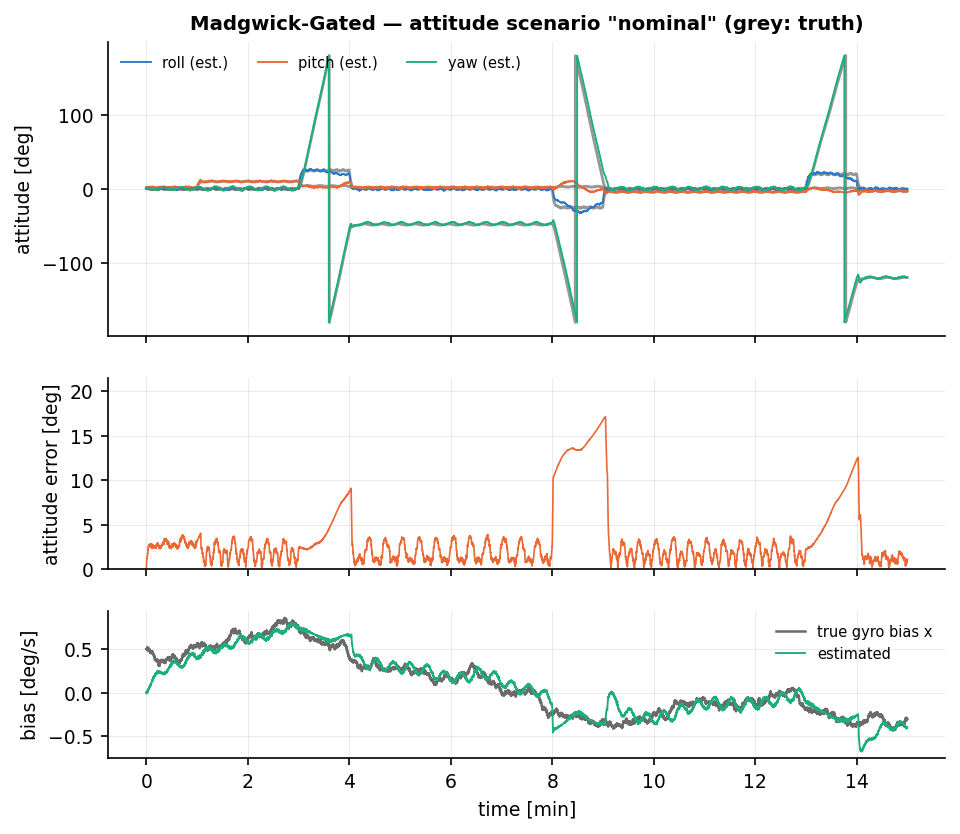
\includegraphics[width=\textwidth]{figures/imu_MadgwickGated_nominal.png}
\caption{Madgwick-Gated on the nominal mission: with the manoeuvre gate the three coordinated turns
are reduced from $\approx40^\circ$ to $5$--$\SI{14}{\degree}$ of error.}
\end{figure}

\texttt{Madgwick-Gated} gives $5.78/6.17/5.79/5.78/3.22/\SI{5.34}{\degree}$ across the six scenarios
in table order, a factor of three better than the published instance, with bias RMSE
$\SI{0.22}{\degree\per\second}$ (against the true $\SI{1.03}{\degree\per\second}$), peak error
$\SI{22.8}{\degree}$ instead of $71.4$, and \emph{no} lost-track flag anywhere. Per phase (seed~1)
\[
2.78\;/\;2.13\;/\;5.08\;/\;2.04\;/\;13.86\;/\;2.08\;/\;7.36\;/\;1.33\ \SI{}{\degree},
\]
so the turns fall from $42/36/\SI{35}{\degree}$ to $5.1/13.9/\SI{7.4}{\degree}$ while the level
phases are unchanged --- the gate does exactly what it is designed to do and nothing else. It is
also the best \texttt{vibration} result of any filter outside the Kalman pair
($\SI{3.22}{\degree}$, $t_{\text{conv}}=\SI{263}{\second}$), because the low-passed magnitude test
correctly declines to treat zero-mean vibration as a manoeuvre.

Two honest caveats. First, the gated filter still does not pass the $2^\circ$ convergence test on
\texttt{nominal}: its floor is $\SI{5.8}{\degree}$, an order of magnitude above the
$\SI{0.65}{\degree}$ sensor floor, because $\beta$ remains a fixed step size and cannot exploit the
much better accelerometer that the gate has now handed it. Compare \texttt{Mahony-Gated}
(Chapter~\ref{ch:att-mahony}), which applies the same gate to a filter whose gain \emph{is}
proportional to the residual and reaches $\SI{2.14}{\degree}$ at the same cost. Second, the
large-initial-error transient is unchanged and still $\beta$-limited: $\SI{5.2}{\second}$ to
$5^\circ$ from $46.6^\circ$, $\SI{13.4}{\second}$ from $78.5^\circ$. The gate buys disturbance
rejection, not bandwidth.

\section{Summary}
Madgwick's filter is the best flops-per-degree bargain in the family in level flight: 272\,bytes,
$\SI{112}{\nano\second}$/step, and $\SI{1.5}{\degree}$--$\SI{2.8}{\degree}$ of error on every phase
that is not a sustained turn. Use it on hand-held, ground or rotary-wing platforms whose specific
force is gravity most of the time. Do not use it on a fixed-wing aircraft without adding manoeuvre
rejection: the constant step size $\beta$ that makes it robust also makes it converge to a wrong
accelerometer at full speed, and the three coordinated turns of this mission cost it a factor of
seven in mission RMS ($17.60$ versus $\SI{2.48}{\degree}$ for the MEKF). If manoeuvre rejection is
added, switch $\zeta$ on with it --- Remark~\ref{rem:mw-package}: the two are worse than useless
apart and give $\SI{5.78}{\degree}$ together, at $\SI{138}{\nano\second}$/step. Neither addition is
Madgwick's; both are ours.

% Copyright 2026 Sreeram Anil
% SPDX-License-Identifier: CC-BY-4.0
% =============================================================================
%  Mahony explicit complementary filter on SO(3) — attitude (AHRS) family
% =============================================================================
\chapter{Explicit Complementary Filter on \texorpdfstring{$SO(3)$}{SO(3)} (Mahony)}
\label{ch:att-mahony}

\section*{At a glance}
\begin{tabular}{@{}l>{\raggedright\arraybackslash}p{0.76\textwidth}@{}}
Family & attitude / AHRS \\
Header & \texttt{include/estkit/attitude/mahony.hpp} \\
Registered names & \texttt{Mahony} (published), \texttt{Mahony-Gated} (practical variant) \\
State & unit quaternion $\bm{q}\in S^3$ and gyro bias $\bm{b}\in\real^3$ (7 reals) \\
Cost per step & $\approx150$ flops, one $\exp$;
  $130$ / $\SI{132}{\nano\second}$ per step, 312\,bytes \\
Tuning & $k_P=1\,\SI{}{\per\second}$, $k_I=0.1\,\SI{}{\per\second\squared}$, $k_a=k_m=1$ \\
Primary references & \cite{mahony2008,hamel2006,euston2008} \\
\end{tabular}

\section{Motivation and aerospace relevance}
The complementary filter of Chapter~\ref{ch:att-complementary} reconstructs an attitude from the
vector observations and then blends two attitudes. Mahony, Hamel and Pflimlin~\cite{mahony2008}
observed that the reconstruction step is unnecessary and, worse, ill-conditioned: what the sensors
actually deliver are \emph{directions}, and directions can be compared directly on $SO(3)$ by a
cross product. Their ``explicit complementary filter'' feeds the weighted sum of those cross
products back as a rate correction, adds an integrator to absorb the gyro bias, and propagates the
estimate with the corrected rate. The result is an observer with a global (more precisely,
almost-global) stability proof, no trigonometry, no matrix inversion and no singularity anywhere.

Two properties make it the standard nonlinear attitude observer in robotics and UAV autopilots.
First, it is \emph{passive}: the innovation term enters as a torque-like feedback and the Lyapunov
argument reduces to a dissipation inequality, so stability does not depend on linearisation.
Second, the bias integrator provides exactly the state that the fixed-gain complementary filter
lacks, at a cost of three extra reals, which removes the $b\tau$ steady-state error
(\eqref{eq:cf-bias}).

The same group's fixed-wing paper~\cite{euston2008} --- the centripetal correction of
Chapter~\ref{ch:att-complementary} --- is the acknowledgement that the observer's assumption
``the accelerometer measures gravity'' is the one thing the proof cannot repair.

\section{Problem statement and assumptions}
Conventions as in Chapter~\ref{ch:att-complementary}. Let $\{\bm{v}_{0i}\}_{i=1}^{n}$ be known unit
directions in the NAV frame and $\bm{v}_i$ their measured BODY counterparts,
\begin{equation}
\bm{v}_i = \bm{R}^\T\bm{v}_{0i} + \text{noise} .
\label{eq:mh-obs}
\end{equation}
Here $n=2$: $\bm{v}_{01}=[0,0,-1]^\T$ with $\bm{v}_1=\bm{f}/\norm{\bm{f}}$, and
$\bm{v}_{02}=\bm{m}_{\text{nav}}/\norm{\bm{m}_{\text{nav}}}$ with $\bm{v}_2=\bm{m}/\norm{\bm{m}}$.
The gyro model is $\bm{\omega}_y=\bm{\omega}+\bm{b}+\bm{n}_v$ with $\bm{b}$ constant or slowly
varying. The filter estimates $(\bm{q},\bm{b})$ and makes no stochastic assumption: it is an
observer, and the gains are chosen by pole placement on the linearised error dynamics rather than
by a Riccati equation.

\section{Derivation}

\subsection{The innovation}
Define the weighted sum of cross products between measured and predicted directions
(Mahony et al.~\cite{mahony2008}, Eq.~(32a)):
\begin{equation}
\hat{\bm{v}}_i = \bm{R}(\hat{\bm{q}})^\T\bm{v}_{0i},
\qquad
\bm{\omega}_{\text{mes}} = \sum_{i=1}^{n} k_i\,\big(\bm{v}_i\times\hat{\bm{v}}_i\big)\ \in\real^3 .
\label{eq:mh-wmes}
\end{equation}
Write the true attitude multiplicatively as $\bm{q}=\hat{\bm{q}}\otimes\exp(\bm{\delta})$ with
$\bm{\delta}\in\real^3$ a BODY-frame rotation vector. Then
$\bm{R}^\T = \exp(-[\bm{\delta}]_\times)\hat{\bm{R}}^\T$ and, to first order,
$\bm{v}_i = \hat{\bm{v}}_i-\bm{\delta}\times\hat{\bm{v}}_i$, so
\begin{align}
\bm{v}_i\times\hat{\bm{v}}_i
 &= -\big(\bm{\delta}\times\hat{\bm{v}}_i\big)\times\hat{\bm{v}}_i + O(\norm{\bm{\delta}}^2)
  = \big(\bm{I}-\hat{\bm{v}}_i\hat{\bm{v}}_i^\T\big)\bm{\delta} + O(\norm{\bm{\delta}}^2),\nonumber\\
\bm{\omega}_{\text{mes}} &= \bm{M}\,\bm{\delta} + O(\norm{\bm{\delta}}^2),
\qquad
\bm{M} := \sum_i k_i\big(\bm{I}-\hat{\bm{v}}_i\hat{\bm{v}}_i^\T\big) = \bm{M}^\T\succeq0 .
\label{eq:mh-lin}
\end{align}
$\bm{M}$ is positive \emph{definite} as soon as two of the $\hat{\bm{v}}_i$ are non-collinear: each
term annihilates only the direction $\hat{\bm{v}}_i$ itself, so the intersection of the null spaces
is empty. That is precisely the observability condition for two-vector attitude determination, and
it fails --- with visible consequences, see Chapter~\ref{ch:att-triad} --- when gravity and the
magnetic field are measured nearly parallel.

\subsection{The filter}
The explicit complementary filter with bias estimation is (\cite{mahony2008}, Eqs.~(32)--(33))
\begin{align}
\dot{\hat{\bm{R}}} &= \hat{\bm{R}}\,\big[\bm{\omega}_y-\hat{\bm{b}}+k_P\,\bm{\omega}_{\text{mes}}\big]_\times ,
 \label{eq:mh-R}\\
\dot{\hat{\bm{b}}} &= -k_I\,\bm{\omega}_{\text{mes}} ,
 \label{eq:mh-b}
\end{align}
with $k_P,k_I>0$. In quaternion form the propagation is the exact exponential map, so the unit norm
is preserved by construction,
\begin{equation}
\hat{\bm{q}}_{k+1} = \hat{\bm{q}}_k\otimes\exp\!\big(\bm{\omega}_c\dt\big),
\qquad \bm{\omega}_c = \bm{\omega}_y-\hat{\bm{b}}+k_P\bm{\omega}_{\text{mes}} .
\label{eq:mh-prop}
\end{equation}

\subsection{Why these signs, and the closed loop}
With $\tilde{\bm{b}}=\bm{b}-\hat{\bm{b}}$ and the noise dropped,
$\bm{\omega}_c = \bm{\omega}+\tilde{\bm{b}}+k_P\bm{\omega}_{\text{mes}}$. Differentiating
$\exp(\bm{\delta})=\hat{\bm{q}}^*\otimes\bm{q}$ and keeping first-order terms,
\begin{equation}
\dot{\bm{\delta}} = \bm{\omega}-\bm{\omega}_c = -k_P\bm{\omega}_{\text{mes}} - \tilde{\bm{b}},
\qquad
\dot{\tilde{\bm{b}}} = -\dot{\hat{\bm{b}}} = +k_I\bm{\omega}_{\text{mes}} .
\label{eq:mh-err}
\end{equation}
Substituting \eqref{eq:mh-lin} gives the linear error system
\begin{equation}
\begin{bmatrix}\dot{\bm{\delta}}\\ \dot{\tilde{\bm{b}}}\end{bmatrix}
=\begin{bmatrix}-k_P\bm{M} & -\bm{I}\\ k_I\bm{M} & \bm{0}\end{bmatrix}
\begin{bmatrix}\bm{\delta}\\ \tilde{\bm{b}}\end{bmatrix},
\qquad\text{characteristic polynomial}\quad
s^2 + k_P\mu\,s + k_I\mu = 0
\label{eq:mh-poly}
\end{equation}
for each eigenvalue $\mu>0$ of $\bm{M}$: a second-order loop with
$\omega_n=\sqrt{k_I\mu}$ and damping $\varsigma = \tfrac12 k_P\sqrt{\mu/k_I}$. The unique
equilibrium is $\bm{\delta}=\bm{0},\ \tilde{\bm{b}}=\bm{0}$, so the observer estimates the bias
correctly --- which the fixed-gain filter of Chapter~\ref{ch:att-complementary}, with
$k_I=0$, cannot. Note that the signs of \eqref{eq:mh-R}--\eqref{eq:mh-b} are not interchangeable:
$+k_P$ in the rate and $-k_I$ in the integrator are what make \eqref{eq:mh-poly} Hurwitz.

\subsection{Lyapunov / passivity argument}
The first-order analysis above is local. The contribution of \cite{mahony2008} is the global one.
With $\bm{E}=\bm{R}\hat{\bm{R}}^\T$ the NAV-frame attitude error and
$\bm{M}_0=\sum_i k_i\bm{v}_{0i}\bm{v}_{0i}^\T$, take
\begin{equation}
V = \sum_i k_i\big(1-\bm{v}_i^\T\hat{\bm{v}}_i\big) + \frac{1}{2k_I}\norm{\tilde{\bm{b}}}^2
  = \tr\!\big(\bm{M}_0(\bm{I}-\bm{E})\big) + \frac{1}{2k_I}\norm{\tilde{\bm{b}}}^2 \;\ge 0 ,
\label{eq:mh-V}
\end{equation}
which vanishes only at $\bm{E}=\bm{I}$, $\tilde{\bm{b}}=\bm{0}$ when $\bm{M}_0$ has full rank.
Differentiating along \eqref{eq:mh-R}--\eqref{eq:mh-b}, the bias terms cancel between the two
channels --- this is the passivity structure: the attitude error supplies
$\bm{\omega}_{\text{mes}}$ to the integrator and the integrator returns $-\tilde{\bm{b}}$ to the
attitude channel through a skew interconnection --- and there remains
\begin{equation}
\dot V = -k_P\,\norm{\bm{\omega}_{\text{mes}}}^2 \;\le\;0 .
\label{eq:mh-Vdot}
\end{equation}
LaSalle's invariance principle applied to \eqref{eq:mh-Vdot} shows that all trajectories converge to
the set $\{\bm{\omega}_{\text{mes}}=\bm{0}\}$, on which $\tilde{\bm{b}}\to\bm{0}$ as well; the
desired equilibrium is locally exponentially stable and the remaining equilibria (rotations by
$\pi$ about the eigenvectors of $\bm{M}_0$) are unstable and form a set of measure zero. This is
Theorem~5.1 of \cite{mahony2008}: \emph{almost-global} asymptotic stability, the strongest result
available on a compact manifold, where global asymptotic stability by a continuous feedback is
topologically impossible.

\subsection{Two optional refinements}
The implementation offers, both off by default:
\emph{(i)} \code{mag\_yaw\_only} --- project $\bm{v}_2\times\hat{\bm{v}}_2$ onto the body-frame
vertical $\hat{\bm{R}}^\T\bm{e}_3$ so that the magnetometer cannot influence roll and pitch;
\emph{(ii)} \code{mag\_ref\_measured} --- rebuild $\bm{v}_{02}$ from the measurement in Madgwick's
way \eqref{eq:mw-flux} instead of using the known field. Both cost accuracy here (results below):
with a \emph{known} reference the magnetometer is a full 3-D observation and contributes to $\bm{M}$
in all directions, and throwing that information away is not free.

\code{mag\_ref\_measured} is nevertheless what \code{ahrs.filters.Mahony} implements, so it is the
setting used for the cross-validation: with it enabled the two implementations agree to
$0.0014^\circ$ maximum angular distance over the $9\times10^4$ samples of the nominal flight
(Table~\ref{tab:val_ahrs}), both scoring $\SI{22.64}{\degree}$ RMS --- against the
$\SI{18.40}{\degree}$ of the registered configuration, which uses the known reference as the 2008
paper does. The residual difference between the two codes is that estkit propagates with the exact
exponential map \eqref{eq:mh-prop} while \code{ahrs} takes an Euler step on $\dot{\bm{q}}$, an
$O(\dt^3)$ effect.

\section{Algorithm}
\begin{algorithm}[H]
\caption{Mahony explicit complementary filter --- one sampling period}
\begin{algorithmic}[1]
\Require $\hat{\bm{q}}_{k-1},\hat{\bm{b}}_{k-1},\bm{\omega}_y,\bm{f},\bm{m}$; $k_P,k_I,k_a,k_m$
\State $\hat{\bm{v}}_1\gets\bm{R}(\hat{\bm{q}})^\T[0,0,-1]^\T$;\;
       $\bm{\omega}_{\text{mes}}\gets k_a\,(\bm{f}/\norm{\bm{f}})\times\hat{\bm{v}}_1$
\State $\hat{\bm{v}}_2\gets\bm{R}(\hat{\bm{q}})^\T\hat{\bm{m}}_{\text{nav}}$;\;
       $\bm{\omega}_{\text{mes}}\mathrel{+}= k_m\,(\bm{m}/\norm{\bm{m}})\times\hat{\bm{v}}_2$
\State $\hat{\bm{b}}\gets\operatorname{clamp}\big(\hat{\bm{b}}-k_I\bm{\omega}_{\text{mes}}\dt\big)$
       \Comment{integrator, \eqref{eq:mh-b}}
\State $\bm{\omega}_c\gets\bm{\omega}_y-\hat{\bm{b}}+k_P\bm{\omega}_{\text{mes}}$
\State $\hat{\bm{q}}_k\gets\hat{\bm{q}}\otimes\exp(\bm{\omega}_c\dt)$, normalise
       \Comment{propagation, \eqref{eq:mh-prop}}
\Ensure $\hat{\bm{q}}_k,\hat{\bm{b}}_k$
\end{algorithmic}
\end{algorithm}

\section{Application to the benchmark flight}
$k_P=\SI{1}{\per\second}$ is the value the assignment prescribes and the one used in the paper's
experiments. With two unit direction measurements and $k_a=k_m=1$, $\bm{M}$ has eigenvalues near
unity, so \eqref{eq:mh-poly} gives $\omega_n=\sqrt{k_I}$ and $\varsigma=k_P/(2\sqrt{k_I})$.
$k_I=\SI{0.1}{\per\second\squared}$ --- the bottom of the assignment's $0.1$--$0.3$ band --- gives
$\omega_n=\SI{0.32}{\radian\per\second}$ and $\varsigma=1.6$: an over-damped attitude loop with a
$\SI{3}{\second}$ time constant and a bias loop of about $\SI{20}{\second}$. The same gains are used
for both registered instances.

$k_I$ was kept at the bottom of the band for a measured reason: the specific-force disturbance of
the coordinated turns drives $\bm{\omega}_{\text{mes}}$ with a long-lived non-zero mean, and the
integrator \eqref{eq:mh-b} converts that into bias error. On \texttt{nominal} the bias RMSE grows
$0.62\to1.25\to2.41\to\SI{2.63}{\degree\per\second}$ as $k_I$ goes $0\to0.1\to0.2\to0.3$, and the
attitude RMS grows with it ($11.97\to18.46\to30.03\to\SI{28.10}{\degree}$).

Everything else is the published algorithm: known inertial reference directions, equal weights, no
manoeuvre rejection.

\section{Implementation notes}
One step is two rotation-matrix--vector products ($2\times9$ MACs, the matrix itself
$\approx20$ flops), two cross products, one clamp and one quaternion exponential: about 150 flops
with a single $\sin/\cos$ pair. Measured $\SI{130}{\nano\second}$/step ($\SI{132}{\nano\second}$
for the gated instance); \code{sizeof} is 312\,bytes. This is the cheapest \emph{bias-estimating}
filter in the family, a factor of 15 below the MEKF.

Numerical hygiene: the quaternion is renormalised inside \code{Quat::integrate}; each branch is
skipped if its measurement magnitude is below $10^{-6}$; the bias state is clamped to
$\pm\SI{10}{\degree\per\second}$, which is the anti-windup that keeps the integrator bounded when the
accelerometer is disturbed for minutes at a time (without it the \texttt{gyro\_bias} run winds past
$\SI{20}{\degree\per\second}$). There is no covariance, hence nothing to keep positive definite, and
the single-precision build reproduces the double-precision mission RMS to four digits.

The limitation is the one the Lyapunov proof makes explicit: \eqref{eq:mh-Vdot} guarantees that the
filter converges to the attitude \emph{consistent with the measured directions}. If the measured
gravity direction is wrong by $23^\circ$ for $\SI{60}{\second}$, the observer converges, correctly
and provably, to the wrong attitude.

\section{Benchmark results}
% Copyright 2026 Sreeram Anil
% SPDX-License-Identifier: CC-BY-4.0
\begin{table}[H]\centering\footnotesize\setlength{\tabcolsep}{3.5pt}\caption{Mahony: attitude benchmark (mean over seeds; all angles in degrees; $t_\mathrm{conv}$: first time the attitude error stays below 2$^\circ$ for 30\,s; bias RMSE in deg/s; 312 bytes of state).}\label{tab:imu_Mahony}
\begin{tabular}{lrrrrrrrrcr}\toprule scenario & RMS & roll & pitch & yaw & max & RMS$_\mathrm{ss}$ & $t_\mathrm{conv}$ [s] & bias RMSE & lost & ns/step \\ \midrule
nominal & 18.40 & 6.24 & 2.94 & 17.30 & 76.3 & 19.33 & 24 & 1.24 & yes & 130 \\
init\_error & 18.51 & 6.28 & 2.98 & 17.41 & 76.3 & 19.33 & 70 & 1.28 & yes & 130 \\
gyro\_bias & 18.44 & 6.25 & 2.94 & 17.35 & 76.3 & 19.33 & 32 & 1.28 & yes & 130 \\
mag\_disturbance & 20.41 & 6.33 & 3.17 & 19.35 & 76.3 & 19.33 & 24 & 1.35 & yes & 130 \\
vibration & 18.28 & 6.23 & 2.95 & 17.17 & 75.6 & 19.25 & 71 & 1.23 & yes & 130 \\
high\_dynamics & 18.75 & 6.42 & 3.01 & 17.63 & 77.3 & 19.62 & -- & 1.26 & yes & 130 \\
\bottomrule\end{tabular}\end{table}

\begin{figure}[H]\centering
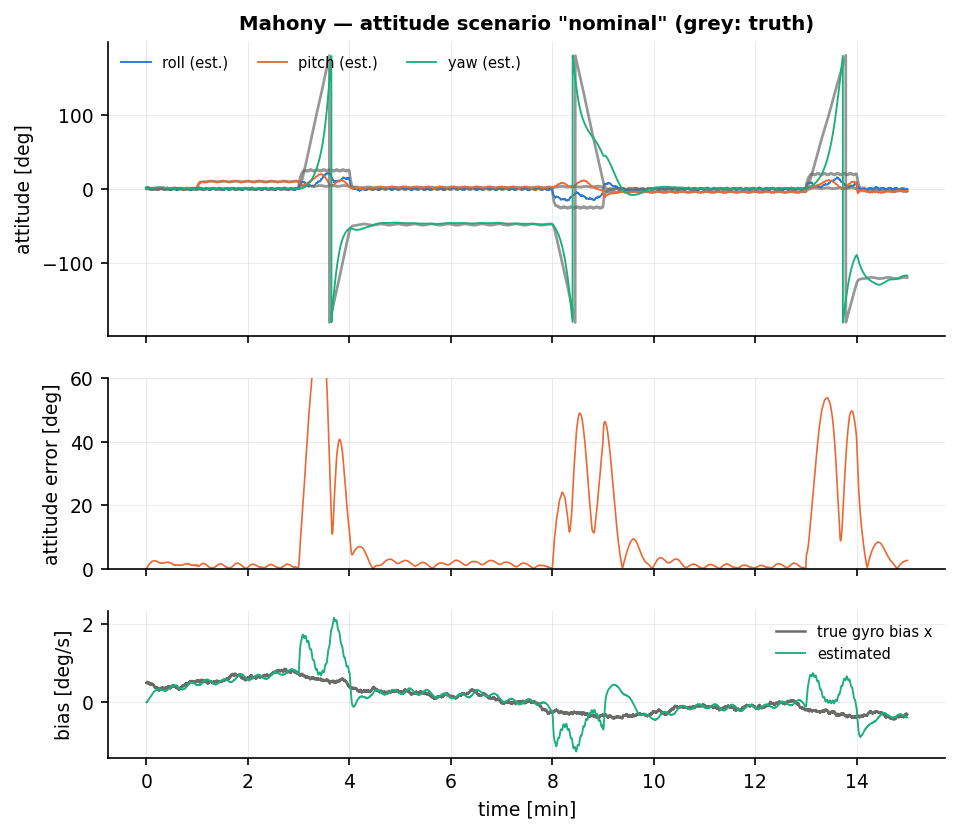
\includegraphics[width=\textwidth]{figures/imu_Mahony_nominal.png}
\caption{Mahony (published, $k_P=1$, $k_I=0.1$) on the nominal mission: the bias integrator
(bottom) is driven by the specific-force disturbance of the turns.}
\end{figure}
\begin{figure}[H]\centering
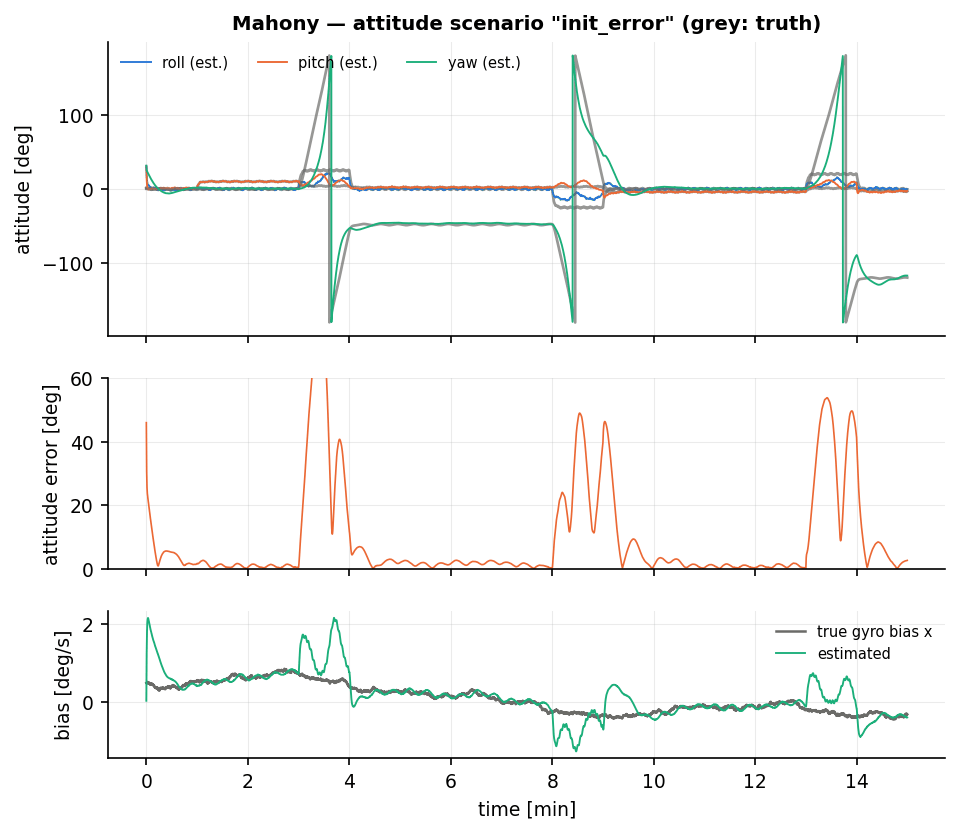
\includegraphics[width=\textwidth]{figures/imu_Mahony_init_error.png}
\caption{Mahony filter with a $46.6^\circ$ initial attitude error.}
\end{figure}

On \texttt{nominal} the published filter gives $\text{RMS}=\SI{18.40}{\degree}$ (roll $6.24$,
pitch $2.94$, yaw $\SI{17.30}{\degree}$), $\text{RMS}_{\text{ss}}=\SI{19.33}{\degree}$, peak
$\SI{76.3}{\degree}$, bias RMSE $\SI{1.24}{\degree\per\second}$, $\SI{130}{\nano\second}$/step and
312\,bytes; it is marked lost on every scenario. Per phase (seed~1),
\[
1.72\;/\;1.06\;/\;\mathbf{45.97}\;/\;2.38\;/\;\mathbf{29.98}\;/\;7.38\;/\;\mathbf{38.18}\;/\;5.46
\ \SI{}{\degree}
\]
for take-off / climb / turn\,1 / cruise / turn\,2 / descent / turn\,3 / final. In level flight it is
the best of the light filters --- $\SI{1.06}{\degree}$ in the climb, well inside the
$\SI{2}{\degree}$ convergence criterion and close to the $\SI{0.65}{\degree}$ sensor floor, because
the $\SI{3}{\second}$ loop averages part of the heading-dependent hard-iron error away --- and in
the turns it is the worst in the family, because the Lyapunov argument does exactly what it
promises. That split also explains the otherwise puzzling $t_{\text{conv}}=\SI{24}{\second}$ in the
table next to a $\SI{19.33}{\degree}$ steady-state RMS: the filter is excellent between the turns
and hopeless inside them.

Table numbers are three-seed means; the gain sweeps below are single-seed (seed~1) diagnostics.

\paragraph{Gain sensitivity.} On \texttt{nominal}, $k_P=0.5/1/2$ at $k_I=0.1$ give
$22.64/18.46/\SI{17.01}{\degree}$ with bias RMSE $1.81/1.25/\SI{0.86}{\degree\per\second}$: a faster
attitude loop leaves less of the disturbance for the integrator. The $k_I$ sweep at $k_P=1$ gives
$11.97/18.46/30.03/\SI{28.10}{\degree}$ for $k_I=0/0.1/0.2/0.3$ with bias RMSE
$0.62/1.25/2.41/\SI{2.63}{\degree\per\second}$. Setting $k_I=0$ (a pure nonlinear complementary
filter, Hamel \& Mahony~\cite{hamel2006}) gives the best \texttt{nominal} number of all,
$\SI{11.97}{\degree}$, but $\SI{20.94}{\degree}$ on \texttt{gyro\_bias} and no bias output at all ---
the integrator is being paid for in disturbance sensitivity and paid back in bias rejection.

\paragraph{Weighting and reference choices.} Reducing the magnetometer weight to $k_m=0.25$ improves
\texttt{nominal} to $\SI{15.78}{\degree}$ and \texttt{mag\_disturbance} to $\SI{18.69}{\degree}$
(from $20.44$): with the accelerometer wrong for a third of the mission, less magnetometer weight
means both less dip-amplified heading error and less exposure to the magnetic disturbance.
\code{mag\_ref\_measured} gives $\SI{22.64}{\degree}$ and \code{mag\_yaw\_only} gives
$\SI{21.76}{\degree}$: both discard the magnetometer's contribution to $\bm{M}$ in the tilt
directions, which on this mission --- where the accelerometer is the unreliable sensor --- is
exactly the wrong information to throw away.

\paragraph{Scenario behaviour.} \texttt{gyro\_bias} ($\SI{3}{\degree\per\second}$) costs almost
nothing in attitude ($\SI{18.44}{\degree}$, $t_{\text{conv}}=\SI{32}{\second}$): the integrator does
its job, and the measured bias RMSE is the same $\SI{1.28}{\degree\per\second}$ as on nominal, i.e.
the integrator tracks the extra $\SI{3}{\degree\per\second}$ and is limited by the turn disturbance,
not by the bias size. \texttt{mag\_disturbance} costs $\SI{2.0}{\degree}$ ($20.41$): with no gating,
the $\SI{25}{\micro\tesla}$ offset enters $\bm{\omega}_{\text{mes}}$ directly and the cruise-phase
RMS rises from $2.38$ to $\SI{17.36}{\degree}$ for the duration. \texttt{vibration} is free
($18.28$): the $k_P$ loop is a $\SI{3}{\second}$ low-pass and averages the extra accelerometer noise
away. \texttt{high\_dynamics} costs $\SI{0.35}{\degree}$ and is the only scenario the published
filter never converges on.

\paragraph{Initial-error transient.} From $46.6^\circ$ the filter reaches $5^\circ$ in
$\SI{8.3}{\second}$ and $1^\circ$ in $\SI{10.3}{\second}$, consistent with the $\SI{3}{\second}$
loop time constant of \eqref{eq:mh-poly} plus the bias-loop settling. From $90^\circ$ it takes
$\SI{1.3}{\second}$ to $5^\circ$ but $\SI{60.7}{\second}$ to $1^\circ$: the large-error correction
is fast (the cross product is largest near $90^\circ$) but the residual bias transient is slow.

\section{The gated variant (\texttt{Mahony-Gated})}\label{sec:mh-gated}
The second registered instance is the same filter --- same $k_P=1$, $k_I=0.1$, same known reference
directions, same Eqs.~\eqref{eq:mh-wmes}--\eqref{eq:mh-prop} --- with \code{gate = true}. This is an
\textbf{engineering addition on top of the published algorithm, not something Mahony, Hamel and
Pflimlin proposed}: the accelerometer weight $k_a$ is multiplied by the disturbance weight
\eqref{eq:cf-weight} of Chapter~\ref{ch:att-complementary}, built from the low-pass-filtered
deviation of $\norm{\bm{f}}$ from $g$ \emph{and} from the rate-driven manoeuvre bound
$V_{\text{ref}}\norm{\bm{\omega}_{yz}}$ of Chapter~\ref{ch:att-mekf},
Remark~\ref{rem:mekf-turn}; beyond a threshold the accelerometer term is dropped from
$\bm{\omega}_{\text{mes}}$ entirely. The Lyapunov argument of \eqref{eq:mh-V}--\eqref{eq:mh-Vdot}
survives the modification --- a time-varying $k_a(t)\ge0$ only changes $\bm{M}$, and
$\dot V=-k_P\norm{\bm{\omega}_{\text{mes}}}^2\le0$ still holds --- but the observability condition
$\bm{M}\succ0$ now fails whenever the accelerometer is gated out, so the guarantee degrades from
almost-global convergence to convergence \emph{while at least two independent directions are
admitted}. The extra cost is $\SI{2}{\nano\second}$/step.

\begin{remark}[Why this is safe here and not for Madgwick]
The manoeuvre detector consumes the bias-compensated rate $\bm{\omega}_y-\hat{\bm{b}}$, so it needs
a bias state to work. Mahony has one by construction, Eq.~\eqref{eq:mh-b}, and the $k_I$ loop
converges in about $\SI{20}{\second}$ --- fast enough that an uncompensated
$\SI{3}{\degree\per\second}$ offset never latches the gate. Madgwick has one only if $\zeta>0$,
which is why \texttt{Madgwick-Gated} must enable both together
(Chapter~\ref{ch:att-madgwick}, Remark~\ref{rem:mw-package}).
\end{remark}

% Copyright 2026 Sreeram Anil
% SPDX-License-Identifier: CC-BY-4.0
\begin{table}[H]\centering\footnotesize\setlength{\tabcolsep}{3.5pt}\caption{Mahony-Gated: attitude benchmark (mean over seeds; all angles in degrees; $t_\mathrm{conv}$: first time the attitude error stays below 2$^\circ$ for 30\,s; bias RMSE in deg/s; 312 bytes of state).}\label{tab:imu_MahonyGated}
\begin{tabular}{lrrrrrrrrcr}\toprule scenario & RMS & roll & pitch & yaw & max & RMS$_\mathrm{ss}$ & $t_\mathrm{conv}$ [s] & bias RMSE & lost & ns/step \\ \midrule
nominal & 2.14 & 0.62 & 0.64 & 1.94 & 8.3 & 2.03 & 24 & 0.14 & no & 132 \\
init\_error & 3.76 & 1.28 & 0.86 & 3.45 & 46.0 & 2.03 & 71 & 0.36 & no & 132 \\
gyro\_bias & 2.74 & 0.80 & 0.63 & 2.54 & 13.1 & 2.03 & 49 & 0.35 & no & 134 \\
mag\_disturbance & 2.31 & 0.66 & 0.66 & 2.10 & 8.7 & 2.03 & 24 & 0.15 & no & 132 \\
vibration & 2.47 & 0.76 & 0.76 & 2.22 & 9.8 & 2.65 & 37 & 0.15 & no & 132 \\
high\_dynamics & 4.83 & 1.55 & 1.11 & 4.41 & 16.5 & 6.07 & 259 & 0.20 & no & 130 \\
\bottomrule\end{tabular}\end{table}

\begin{figure}[H]\centering
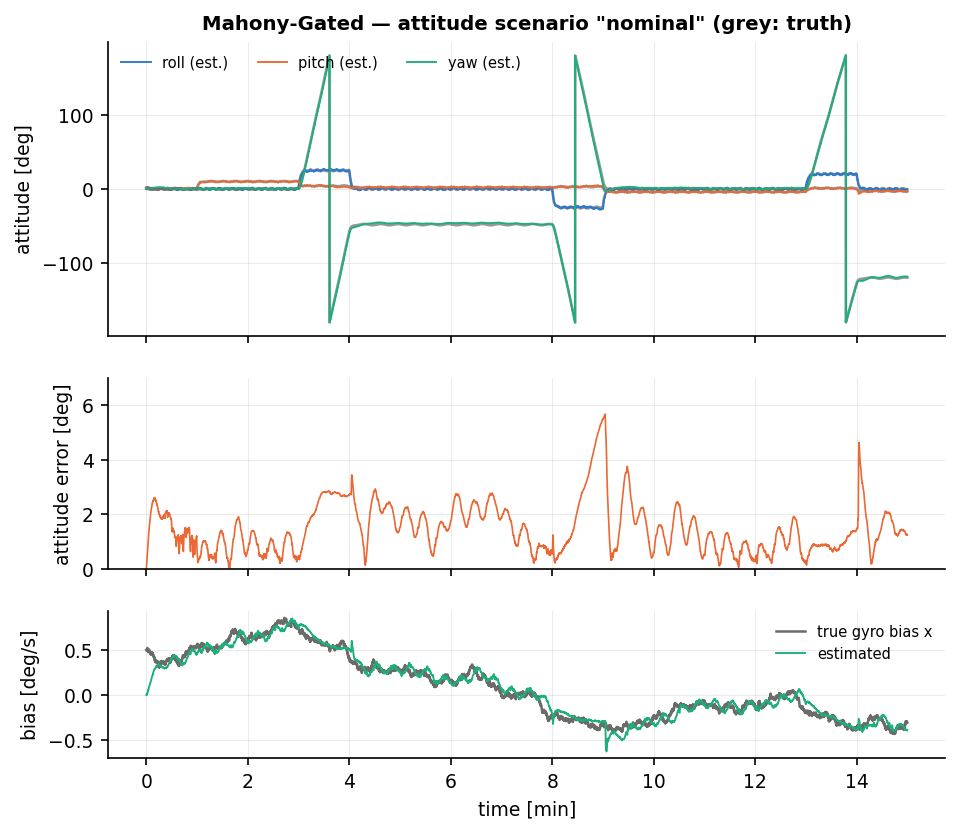
\includegraphics[width=\textwidth]{figures/imu_MahonyGated_nominal.png}
\caption{Mahony-Gated on the nominal mission: the same observer with a manoeuvre-gated
accelerometer weight. The turns are no longer visible in the error trace.}
\end{figure}

\texttt{Mahony-Gated} is the single largest improvement in this family:
$2.14/3.76/2.74/2.31/2.47/\SI{4.83}{\degree}$ across the six scenarios in table order, against
$18.40/18.51/18.44/20.41/18.28/\SI{18.75}{\degree}$ for the published filter --- a factor of
\emph{nine} on \texttt{nominal} --- with roll $0.62$, pitch $0.64$, yaw $\SI{1.94}{\degree}$, peak
error $\SI{8.3}{\degree}$ instead of $76.3$, $\text{RMS}_{\text{ss}}=\SI{2.03}{\degree}$, bias RMSE
$\SI{0.14}{\degree\per\second}$ (against a true $\SI{1.03}{\degree\per\second}$), no lost-track flag
on any scenario, and $\SI{132}{\nano\second}$/step at 312\,bytes. Per phase (seed~1),
\[
1.64\;/\;0.93\;/\;2.43\;/\;1.83\;/\;3.14\;/\;1.40\;/\;1.28\;/\;1.68\ \SI{}{\degree}
\]
--- the turns are no longer distinguishable from the cruise. It is the best estimator in the family
on \texttt{nominal} and \texttt{mag\_disturbance}, better than the MEKF ($2.48$ and $2.86$) at
\emph{one fifteenth} of the cost, and it reaches the $2^\circ$ convergence criterion at
$t=\SI{24}{\second}$.

This is the most important measurement in the chapter, and it should be read as a statement about
\emph{disturbance modelling}, not about estimator structure: the $\SI{16}{\degree}$ that separates
\texttt{Mahony} from \texttt{MEKF} in the overview table is almost entirely a difference in what the
two filters believe about the accelerometer during a coordinated turn, not in how they represent
attitude or propagate a covariance. Give the 1\,kB nonlinear observer the same belief and it matches
the $6\times6$ Kalman filter.

Three caveats, in the interest of not overselling it. \emph{(i)} On \texttt{high\_dynamics} the gated
filter degrades to $\SI{4.83}{\degree}$ --- worse, relative to its own baseline, than the MEKF's
$3.33$ --- because with tripled turbulence the gate fires often and a fixed-gain filter has no
covariance with which to re-weight what remains. \emph{(ii)} The large-initial-error transient gets
\emph{worse}: from $46.6^\circ$ the gated filter needs $\SI{16.5}{\second}$ to reach $5^\circ$
against the ungated $\SI{8.3}{\second}$, and $\SI{24.6}{\second}$ from $78.5^\circ$ against
$\SI{8.7}{\second}$, because the de-rated $k_a$ slows the attitude loop exactly when the innovation
is largest --- a fixed-gain filter cannot tell ``large residual because the state is wrong'' from
``large residual because the measurement is wrong''. This shows up in the table as
\texttt{init\_error} being its worst non-dynamic scenario ($3.76$ against $\SI{2.14}{\degree}$) and
$t_{\text{conv}}$ slipping from $24$ to $\SI{71}{\second}$. \emph{(iii)} The gate introduces two
constants ($V_{\text{ref}}$ and the editing threshold) that the published filter does not have, and
they encode an assumption about the airframe.

\section{Summary}
The Mahony filter is the right default nonlinear attitude observer: 312\,bytes,
$\SI{0.13}{\micro\second}$/step, an almost-global stability proof, and a bias state that removes the
fixed-gain filter's $b\tau$ error. Its gains are two numbers with a textbook second-order
interpretation, \eqref{eq:mh-poly}. Use it whenever the vector observations can be trusted on
average. Do not use it unmodified where they cannot: the same Lyapunov function that guarantees
convergence guarantees convergence \emph{to the disturbed solution}, which on this fixed-wing
mission costs a factor of nine in RMS and an order of magnitude in bias accuracy. Add manoeuvre
rejection --- the separately registered \texttt{Mahony-Gated} --- and it becomes, measurably,
\emph{better} than the MEKF on \texttt{nominal} and \texttt{mag\_disturbance} and within
$\SI{1.5}{\degree}$ of it on the rest, at a fifteenth of the price, at the cost of
two airframe constants and a slower large-error transient.

% Copyright 2026 Sreeram Anil
% SPDX-License-Identifier: CC-BY-4.0
% =============================================================================
%  Multiplicative extended Kalman filter — attitude (AHRS) family
% =============================================================================
\chapter{Multiplicative Extended Kalman Filter (MEKF)}
\label{ch:att-mekf}

\section*{At a glance}
\begin{tabular}{@{}l>{\raggedright\arraybackslash}p{0.76\textwidth}@{}}
Family & attitude / AHRS \\
Header & \texttt{include/estkit/attitude/mekf.hpp} \\
Registered name & \texttt{MEKF} \\
State & $\hat{\bm{q}}\in S^3$, $\hat{\bm{b}}\in\real^3$; error
 $[\delta\bm{\theta};\delta\bm{b}]\in\real^6$, $\mP\in\real^{6\times6}$ \\
Cost per step & $\approx2.9\times10^3$ MACs; $\SI{2.04}{\micro\second}$/step, 608\,bytes \\
Primary references & \cite{lefferts1982,markley2003mekf,crassidis2007survey,farrenkopf1978,bucyjoseph1968} \\
\end{tabular}

\section{Motivation and aerospace relevance}
Attitude is the canonical example of a state that does not live in a vector space. A quaternion has
four components and three degrees of freedom; an ordinary EKF that carries a $4\times4$ covariance
for it is describing a distribution on $\real^4$ whose support is a three-dimensional sphere, so
$\mP$ is necessarily singular in the radial direction and the filter must fight the norm constraint
at every step. Lefferts, Markley and Shuster~\cite{lefferts1982} settled the matter for spacecraft
in 1982: keep the quaternion as a \emph{reference} that carries the large, nonlinear part of the
attitude, and let the Kalman filter estimate only a small three-parameter \emph{error} that is
composed with it multiplicatively. The covariance is then a genuine $3\times3$ (or, with the gyro
bias, $6\times6$) object with no constraint attached.

Markley~\cite{markley2003mekf} showed that all the usual three-parameter error representations ---
rotation vector, Gibbs vector, modified Rodrigues parameters, the quaternion vector part --- agree
to second order and differ only in how the reset step is implemented, so the choice is a matter of
taste rather than accuracy. Crassidis, Markley and Cheng~\cite{crassidis2007survey} survey what came
afterwards, of which the unscented variant~\cite{crassidismarkley2003} is the closest relative;
the MEKF remains the reference against which everything is compared, and it flies on
essentially every spacecraft and every high-grade AHRS.

For a battery-management toolbox the MEKF is the aerospace half of the same idea that makes the
error-state formulation attractive in Chapter~\ref{ch:ekf}: linearise the \emph{deviation}, not the
state, so that the operating point never has to be re-derived.

\section{Problem statement and assumptions}
Conventions as in Chapter~\ref{ch:att-complementary}; $\bm{R}$ denotes a rotation and measurement
covariances are written $\bm{\Sigma}$.

\paragraph{Process model.} The gyro is treated as an \emph{input}, not as a measurement of a
dynamic model --- there is no vehicle model at all. With the Farrenkopf~\cite{farrenkopf1978} gyro
error model,
\begin{equation}
\bm{\omega}_y = \bm{\omega} + \bm{b} + \bm{n}_v,\qquad
\dot{\bm{b}} = \bm{n}_u,\qquad
\bm{n}_v\sim\N{\bm{0}}{\sigma_v^2\bm{I}\,\delta(t-\tau)},\quad
\bm{n}_u\sim\N{\bm{0}}{\sigma_u^2\bm{I}\,\delta(t-\tau)} ,
\label{eq:mekf-gyro}
\end{equation}
$\sigma_v$ is the angle random walk (rad\,s$^{-1/2}$) and $\sigma_u$ the rate random walk
(rad\,s$^{-3/2}$). The attitude obeys $\dot{\bm{q}}=\tfrac12\bm{q}\otimes[0,\bm{\omega}]$.

\paragraph{Measurement model.} Any body-frame observation of a known NAV vector $\bm{r}$,
\begin{equation}
\bm{y} = \bm{R}^\T\bm{r} + \bm{n},\qquad \bm{n}\sim\N{\bm{0}}{\bm{\Sigma}} .
\label{eq:mekf-meas}
\end{equation}
Two are used: $\bm{r}_a=[0,0,-g]^\T$ with $\bm{y}=\bm{f}$, and $\bm{r}_m=\bm{m}_{\text{nav}}$ with
$\bm{y}=\bm{m}$.

\paragraph{The multiplicative error.} Define
\begin{equation}
\bm{q} = \hat{\bm{q}}\otimes\exp(\delta\bm{\theta}),\qquad
\bm{b} = \hat{\bm{b}} + \delta\bm{b},\qquad
\bm{x} = \begin{bmatrix}\delta\bm{\theta}\\ \delta\bm{b}\end{bmatrix}\in\real^6,\qquad
\bm{x}\sim\N{\bm{0}}{\mP} .
\label{eq:mekf-err}
\end{equation}
$\delta\bm{\theta}$ is a BODY-frame rotation vector. Between updates $\bm{x}\equiv\bm{0}$ by
construction (the reset of \S\ref{sec:mekf-reset} pushes every correction into
$\hat{\bm{q}},\hat{\bm{b}}$), so the three-parameter representation never has to describe a large
rotation and $\mP$ never becomes singular.

\section{Derivation}

\subsection{Error kinematics}
Let $\hat{\bm{\omega}}=\bm{\omega}_y-\hat{\bm{b}}$ be the estimated rate. Write
$\delta\bm{q}=\hat{\bm{q}}^*\otimes\bm{q}$ and differentiate:
\begin{equation}
\dot{\delta\bm{q}} = \dot{\hat{\bm{q}}}^*\otimes\bm{q} + \hat{\bm{q}}^*\otimes\dot{\bm{q}}
 = \tfrac12\big(\delta\bm{q}\otimes[0,\bm{\omega}] - [0,\hat{\bm{\omega}}]\otimes\delta\bm{q}\big).
\label{eq:mekf-dq}
\end{equation}
Substituting $\delta\bm{q}=[1,\tfrac12\delta\bm{\theta}]+O(\norm{\delta\bm{\theta}}^2)$ and
$\bm{\omega}=\hat{\bm{\omega}}+\Delta\bm{\omega}$, the scalar parts cancel and the vector part of
\eqref{eq:mekf-dq} gives
\begin{equation}
\dot{\delta\bm{\theta}} = -\hat{\bm{\omega}}\times\delta\bm{\theta} + \Delta\bm{\omega}
 = -[\hat{\bm{\omega}}]_\times\,\delta\bm{\theta} - \delta\bm{b} - \bm{n}_v ,
\label{eq:mekf-dtheta}
\end{equation}
because $\Delta\bm{\omega}=\bm{\omega}-\hat{\bm{\omega}}
=(\bm{\omega}_y-\bm{b}-\bm{n}_v)-(\bm{\omega}_y-\hat{\bm{b}})=-\delta\bm{b}-\bm{n}_v$. Together with
$\dot{\delta\bm{b}}=\bm{n}_u$,
\begin{equation}
\dot{\bm{x}} = \mF\bm{x} + \mG\bm{n},\qquad
\mF=\begin{bmatrix}-[\hat{\bm{\omega}}]_\times & -\bm{I}\\ \bm{0}&\bm{0}\end{bmatrix},\qquad
\mG=\begin{bmatrix}-\bm{I}&\bm{0}\\ \bm{0}&\bm{I}\end{bmatrix},\qquad
\bm{n}=\begin{bmatrix}\bm{n}_v\\ \bm{n}_u\end{bmatrix}.
\label{eq:mekf-F}
\end{equation}

\subsection{Discrete transition matrix}
$\mF$ is block upper triangular with a nilpotent lower-right block, and $[\hat{\bm{\omega}}]_\times$
is constant over one sample, so $\bm{\Phi}=\exp(\mF\dt)$ can be written in closed form. With
$\bm{a}=\hat{\bm{\omega}}\dt$, $\vartheta=\norm{\bm{a}}$,
\begin{align}
\bm{\Phi}_{11} &= \exp\!\big(-[\bm{a}]_\times\big)
 = \bm{I} - \frac{\sin\vartheta}{\vartheta}[\bm{a}]_\times
  + \frac{1-\cos\vartheta}{\vartheta^2}[\bm{a}]_\times^2 ,
 \label{eq:mekf-phi11}\\
\bm{\Phi}_{12} &= -\!\int_0^{\dt}\!\exp\!\big(-[\hat{\bm{\omega}}]_\times\tau\big)\,d\tau
 = -\dt\left(\bm{I} - \frac{1-\cos\vartheta}{\vartheta^2}[\bm{a}]_\times
  + \frac{\vartheta-\sin\vartheta}{\vartheta^3}[\bm{a}]_\times^2\right),
 \label{eq:mekf-phi12}
\end{align}
with $\bm{\Phi}_{21}=\bm{0}$, $\bm{\Phi}_{22}=\bm{I}$ (Lefferts et al.~\cite{lefferts1982},
Eq.~(2.9); Markley \& Crassidis~\cite{markleycrassidis2014}, Eq.~(6.60)). The series limits
$\sin\vartheta/\vartheta\to1$, $(1-\cos\vartheta)/\vartheta^2\to\tfrac12$,
$(\vartheta-\sin\vartheta)/\vartheta^3\to\tfrac16$ are used below $\vartheta=10^{-6}$.

\subsection{Discrete process noise (Farrenkopf's model)}
Van Loan's construction~\cite{vanloan1978} applied to \eqref{eq:mekf-F} with
$[\hat{\bm{\omega}}]_\times$ neglected inside the integral (its effect is $O(\vartheta^2)$ relative,
$<10^{-5}$ at $\SI{100}{\hertz}$) gives, with $\bm{\Phi}(\tau)=\big[\begin{smallmatrix}\bm{I}&-\tau\bm{I}\\ \bm{0}&\bm{I}\end{smallmatrix}\big]$,
\begin{equation}
\mQ_d=\int_0^{\dt}\bm{\Phi}(\tau)\,\mG\begin{bmatrix}\sigma_v^2\bm{I}&\\&\sigma_u^2\bm{I}\end{bmatrix}\mG^\T\bm{\Phi}(\tau)^\T d\tau
=\begin{bmatrix}
 \big(\sigma_v^2\dt+\tfrac13\sigma_u^2\dt^3\big)\bm{I} & -\tfrac12\sigma_u^2\dt^2\,\bm{I}\\[2pt]
 -\tfrac12\sigma_u^2\dt^2\,\bm{I} & \sigma_u^2\dt\,\bm{I}
\end{bmatrix},
\label{eq:mekf-Q}
\end{equation}
the classical Farrenkopf~\cite{farrenkopf1978} result. The negative cross-term is not cosmetic: it
encodes the fact that an over-estimated bias produces a \emph{negative} attitude drift, and dropping
it makes the filter optimistic about how quickly the bias becomes observable.

\paragraph{Units.} The benchmark configuration supplies \emph{per-sample} standard deviations: the
gyro noise is added once per sample with standard deviation $\sigma_d$, and the bias increment once
per sample with standard deviation $\sigma_{rw}$. The angle accumulated from gyro noise in one step
is $\sigma_d\dt$, and \eqref{eq:mekf-Q} says it is $\sigma_v\sqrt{\dt}$; the bias increment is
$\sigma_u\sqrt{\dt}$. Hence
\begin{equation}
\sigma_v = \sigma_d\sqrt{\dt},\qquad \sigma_u = \sigma_{rw}/\sqrt{\dt} ,
\label{eq:mekf-units}
\end{equation}
which for the nominal scenario gives
$\sigma_v = \SI{1.75e-3}{\radian\per\second}\times0.1 = \SI{1.75e-4}{}$ and
$\sigma_u=\SI{3.49e-5}{}\times10=\SI{3.49e-4}{}$ in SI units. Getting
\eqref{eq:mekf-units} wrong by the factor $\dt$ is the single most common error in AHRS tuning; it
scales $\mQ$ by $10^4$ here.

\subsection{Measurement Jacobian}
From $\bm{R}(\hat{\bm{q}}\otimes\exp(\delta\bm{\theta}))=\hat{\bm{R}}\exp([\delta\bm{\theta}]_\times)
\approx\hat{\bm{R}}(\bm{I}+[\delta\bm{\theta}]_\times)$ we get
$\bm{R}^\T\approx(\bm{I}-[\delta\bm{\theta}]_\times)\hat{\bm{R}}^\T$, hence for \eqref{eq:mekf-meas}
\begin{equation}
\bm{y} \approx \hat{\bm{R}}^\T\bm{r} - \delta\bm{\theta}\times(\hat{\bm{R}}^\T\bm{r}) + \bm{n}
 = \underbrace{\hat{\bm{R}}^\T\bm{r}}_{\hat{\bm{y}}}
  + \underbrace{\big[\hat{\bm{R}}^\T\bm{r}\big]_\times}_{\mH_{\delta\theta}}\delta\bm{\theta} + \bm{n},
\qquad
\mH = \big[\;[\hat{\bm{R}}^\T\bm{r}]_\times \;\;\bm{0}_{3\times3}\;\big] .
\label{eq:mekf-H}
\end{equation}
$\mH$ has rank 2: a rotation about $\hat{\bm{R}}^\T\bm{r}$ leaves the observation unchanged, which
is why a single vector observation can never fix the attitude. Two non-collinear observations give
$\mH\in\real^{6\times6}$ of rank 3 in the attitude block and the attitude becomes observable
instantaneously; the bias block is observable only through the coupling $\bm{\Phi}_{12}$, i.e. over
time.

\subsection{Update and reset}\label{sec:mekf-reset}
Stacking the accelerometer and magnetometer blocks, the update is the textbook one about the
\emph{zero} prior error state:
\begin{align}
\bm{z} &= \begin{bmatrix}\bm{f}-\hat{\bm{R}}^\T\bm{r}_a\\ \bm{m}-\hat{\bm{R}}^\T\bm{r}_m\end{bmatrix},
\qquad
\mS = \mH\mP\mH^\T+\bm{\Sigma},\qquad \mK=\mP\mH^\T\mS\inv,\label{eq:mekf-K}\\
\bm{x}^+ &= \mK\bm{z},\qquad
\Pplus = (\mI-\mK\mH)\Pminus(\mI-\mK\mH)^\T + \mK\bm{\Sigma}\mK^\T ,\label{eq:mekf-P}
\end{align}
the Joseph form~\cite{bucyjoseph1968}, followed immediately by the \emph{reset} that returns the
error state to zero (Markley~\cite{markley2003mekf}, Sec.~V):
\begin{equation}
\hat{\bm{q}} \leftarrow \hat{\bm{q}}\otimes\exp\!\big(\delta\bm{\theta}^+\big),\qquad
\hat{\bm{b}} \leftarrow \hat{\bm{b}} + \delta\bm{b}^+,\qquad
\bm{x}\leftarrow\bm{0} .
\label{eq:mekf-reset}
\end{equation}
The reset is what makes the filter \emph{multiplicative}: the large rotation is absorbed by a
quaternion product, which is exact, and only the residual --- now zero --- is carried in the linear
state. To first order the reset leaves $\mP$ unchanged; the second-order correction
$\Pplus_{11}\leftarrow(\bm{I}-\tfrac12[\delta\bm{\theta}^+]_\times)\Pplus_{11}(\cdot)^\T$ is
$O(\norm{\delta\bm{\theta}^+}^2)$ and, as in every standard implementation, omitted.

\subsection{Measurement covariance: the part that is not textbook}
\label{sec:mekf-R}
For an AHRS the sensor noise is not the dominant error of \eqref{eq:mekf-meas} --- the \emph{model}
is. The accelerometer measures $\bm{R}^\T(\bm{a}_{\text{nav}}-\bm{g}_{\text{nav}})$ and the filter
pretends it measures $-\bm{R}^\T\bm{g}_{\text{nav}}$; the magnetometer sees hard-iron and local
field errors. $\bm{\Sigma}$ is therefore built as
\begin{equation}
\bm{\Sigma}_a = \big(\sigma_a^2+\sigma_{a,\text{extra}}^2+\sigma_{x,a}^2\big)\bm{I},\qquad
\bm{\Sigma}_m = \big(\sigma_m^2+\sigma_{m,\text{extra}}^2+\sigma_{x,m}^2\big)\bm{I},
\label{eq:mekf-R}
\end{equation}
with the disturbance terms
\begin{equation}
\sigma_{x,a} = \sqrt{\big(k_a\,e_a\big)^2 + \big(V_{\text{ref}}\max(0,\norm{\bm{\omega}_{yz}}-\varpi)\big)^2},
\qquad
\sigma_{x,m} = k_m\,e_m ,
\label{eq:mekf-sx}
\end{equation}
where $e_a,e_m$ are the low-pass-filtered magnitude anomalies of \eqref{eq:cf-weight} and
$\bm{\omega}_{yz}$ is the $(y,z)$ part of the bias-compensated rate.

The second term of $\sigma_{x,a}$ deserves its own statement, because a magnitude check alone does
\emph{not} work.
\begin{remark}[A coordinated turn is invisible to a norm test]\label{rem:mekf-turn}
In a coordinated turn at bank $\phi$ the specific force stays aligned with the body $z$ axis and has
magnitude $g/\cos\phi$. At $\phi=25^\circ$ that is $1.10\,g$: the \emph{direction} is wrong by
$25^\circ$ while the \emph{magnitude} is wrong by $10\,\%$, i.e. by
$\SI{1}{\metre\per\second\squared}$, comparable to ordinary turbulence. What does reveal the
condition is the rate: from $\bm{f}=\dot{\bm{v}}_b+\bm{\omega}\times\bm{v}_b-\bm{R}^\T\bm{g}$ the
unmodelled part is bounded by $\norm{\bm{\omega}\times\bm{v}_b}=V\norm{\bm{\omega}_{yz}}$ for an
aircraft flying along its $x$ axis. Bounding $V$ by the airframe's nominal airspeed
$V_{\text{ref}}$ --- a design constant, not a measurement --- gives a rate-driven standard deviation
that inflates $\bm{\Sigma}_a$ exactly when the aircraft manoeuvres. This is the covariance version
of the Euston et al.~\cite{euston2008} correction used in Chapter~\ref{ch:att-complementary}: it
widens the uncertainty instead of correcting the mean, and needs no airspeed sensor.
\end{remark}
The dead-zone $\varpi$ covers the residual rate uncertainty (bias plus noise). Without it an
uncompensated gyro bias would appear as a permanent manoeuvre and switch the accelerometer off for
ever --- a dead-lock, since the bias estimate needs the accelerometer.

Finally, and equally importantly, \eqref{eq:mekf-R} is capped by \emph{editing}: if
$\sigma_{x,a}$ exceeds a threshold, the accelerometer block is skipped entirely (formally
$\bm{\Sigma}_a\to\infty$), and likewise for the magnetometer. The reason is that a manoeuvre or a
magnetic anomaly is a \emph{systematic} error lasting thousands of samples, not white noise: with a
merely inflated but finite $\bm{\Sigma}$, the Kalman filter accumulates $N$ correlated samples and
converges to the biased answer with effective standard deviation $\sigma/\sqrt{N}$. Measurement
editing is the standard treatment (Gelb~\cite[Sec.~4.5]{gelb1974};
Tapley et al.~\cite[Sec.~4.15]{tapley2004}) and is worth a factor of $2.5$ here (results below).

\section{Algorithm}
\begin{algorithm}[H]
\caption{MEKF --- one sampling period}
\begin{algorithmic}[1]
\Require $\hat{\bm{q}},\hat{\bm{b}},\mP$; $\bm{\omega}_y,\bm{f},\bm{m}$; $\sigma_v,\sigma_u,\bm{\Sigma}$ parameters
\State \textbf{Time update:} $\hat{\bm{\omega}}\gets\bm{\omega}_y-\hat{\bm{b}}$;\;
       $\hat{\bm{q}}\gets\hat{\bm{q}}\otimes\exp(\hat{\bm{\omega}}\dt)$, normalise
\State $\bm{\Phi}\gets$ \eqref{eq:mekf-phi11}--\eqref{eq:mekf-phi12};\;
       $\mQ_d\gets$ \eqref{eq:mekf-Q};\;
       $\mP\gets\bm{\Phi}\mP\bm{\Phi}^\T+\mQ_d$; symmetrise
\State \textbf{Measurement update:} $\hat{\bm{y}}_a\gets\hat{\bm{R}}^\T\bm{r}_a$,\;
       $\hat{\bm{y}}_m\gets\hat{\bm{R}}^\T\bm{r}_m$
\State $\bm{\Sigma}\gets$ \eqref{eq:mekf-R}--\eqref{eq:mekf-sx}; \textbf{edit} blocks whose
       disturbance exceeds the threshold
\State $\mH\gets\big[\begin{smallmatrix}[\hat{\bm{y}}_a]_\times&\bm{0}\\ [\hat{\bm{y}}_m]_\times&\bm{0}\end{smallmatrix}\big]$;\;
       $\bm{z}\gets[\bm{f}-\hat{\bm{y}}_a;\;\bm{m}-\hat{\bm{y}}_m]$
\State $\mS\gets\mH\mP\mH^\T+\bm{\Sigma}$;\; $\mK\gets\mP\mH^\T\mS\inv$;\;
       \textbf{if} $\mK$ not finite \textbf{then return}
\State $\bm{x}^+\gets\mK\bm{z}$;\;
       $\mP\gets(\mI-\mK\mH)\mP(\mI-\mK\mH)^\T+\mK\bm{\Sigma}\mK^\T$; symmetrise
\State \textbf{Reset:} $\hat{\bm{q}}\gets\hat{\bm{q}}\otimes\exp(\delta\bm{\theta}^+)$, normalise;\;
       $\hat{\bm{b}}\gets\operatorname{clamp}(\hat{\bm{b}}+\delta\bm{b}^+)$
\Ensure $\hat{\bm{q}},\hat{\bm{b}},\mP$
\end{algorithmic}
\end{algorithm}

\section{Application to the benchmark flight}
$\mQ$ comes straight from the configuration through \eqref{eq:mekf-units}; nothing is tuned there
($q_{\text{scale}}=1$). $\mP_0=\diag\big((30^\circ)^2\bm{I},(\SI{3}{\degree\per\second})^2\bm{I}\big)$:
a $30^\circ$ initial attitude uncertainty is the standard ``unknown coarse alignment'' value and
covers the $46.6^\circ$ of the \texttt{init\_error} scenario, and
$\SI{3}{\degree\per\second}$ of bias uncertainty covers the \texttt{gyro\_bias} scenario.

Only $\bm{\Sigma}$ carries engineering judgement:
$\sigma_{a,\text{extra}}=\SI{0.5}{\metre\per\second\squared}$ (about $3^\circ$ of tilt) for the
residual linear acceleration of ordinary flight;
$\sigma_{m,\text{extra}}=\SI{1.5}{\micro\tesla}$ for the airframe's field-model error (a
deliberately conservative figure: the dataset's residual hard iron after calibration is only
$\SI{0.42}{\micro\tesla}$, and the registry comment quoting $\SI{1.37}{\micro\tesla}$ predates the
compass recalibration --- see the sensitivity study below, where the value turns out not to matter
on any scenario except \texttt{init\_error});
$V_{\text{ref}}=\SI{45}{\metre\per\second}$ (the nominal cruise airspeed) and
$\varpi=\SI{0.02}{\radian\per\second}$ for the manoeuvre bound; editing thresholds
$\SI{1}{\metre\per\second\squared}$ and $\SI{3}{\micro\tesla}$. The centripetal \emph{mean}
correction is available as an option but is switched \textbf{off}: see the results.

\section{Implementation notes}
Per step: $\bm{\Phi}\mP\bm{\Phi}^\T$ is $2\times216$ MACs, $\mH\mP\mH^\T$ another $432$, the
$6\times6$ LU inverse about $290$, $\mP\mH^\T\mS\inv$ $432$, and the Joseph form $1080$ --- about
$2.9\times10^3$ multiply--adds in total, plus two $3\times3$ rotation matrices and one quaternion
exponential. Measured $\SI{2.04}{\micro\second}$/step, 15 times the Mahony filter and
still three orders of magnitude inside the $\SI{10}{\milli\second}$ budget at $\SI{100}{\hertz}$; on
a $\SI{216}{\mega\hertz}$ Cortex-M7 in float32 this is of order $\SI{40}{\micro\second}$, i.e.
$0.4\,\%$ duty. \code{sizeof} is 608\,bytes, dominated by the $6\times6$ covariance (288\,B).

The right half of $\mH$ is structurally zero and both blocks are $3\times3$ skew matrices; a
hand-rolled version exploiting that, and doing two sequential $3$-dimensional updates instead of one
$6$-dimensional one, would cut the cost roughly in half and remove the $6\times6$ inverse. The
generic form was kept because it is what \code{linalg.hpp} expresses naturally and because the
sequential form is not algebraically identical when the two blocks are correlated through $\mP$.

Numerical hygiene: $\mP$ is symmetrised after both the time and the measurement update; the Joseph
form is used (\code{joseph=true}); the gain and the correction are checked with \code{is\_finite()}
and the update is skipped rather than propagating NaN; the quaternion is renormalised after the
reset; the bias is clamped to $\pm\SI{15}{\degree\per\second}$; $\bm{\Phi}$ falls back to its series
form below $\vartheta=10^{-6}$. Measured: \code{joseph=false} and \code{exact\_phi=false} both give
\emph{bit-identical} mission statistics here ($\SI{2.11}{\degree}$, seed~1), which says that at
$\SI{100}{\hertz}$ with $\norm{\bm{\omega}}\dt<10^{-3}$ neither the second-order terms of
\eqref{eq:mekf-phi11} nor the Joseph stabilisation is being exercised --- they are insurance, not
accuracy. The single-precision build reproduces the double-precision RMS to four digits.

\section{Benchmark results}
% Copyright 2026 Sreeram Anil
% SPDX-License-Identifier: CC-BY-4.0
\begin{table}[H]\centering\footnotesize\setlength{\tabcolsep}{3.5pt}\caption{MEKF: attitude benchmark (mean over seeds; all angles in degrees; $t_\mathrm{conv}$: first time the attitude error stays below 2$^\circ$ for 30\,s; bias RMSE in deg/s; 608 bytes of state).}\label{tab:imu_MEKF}
\begin{tabular}{lrrrrrrrrcr}\toprule scenario & RMS & roll & pitch & yaw & max & RMS$_\mathrm{ss}$ & $t_\mathrm{conv}$ [s] & bias RMSE & lost & ns/step \\ \midrule
nominal & 2.48 & 0.84 & 0.68 & 2.23 & 15.1 & 3.07 & 0 & 0.17 & no & 2037 \\
init\_error & 2.50 & 0.85 & 0.68 & 2.25 & 15.1 & 3.07 & 3 & 0.25 & no & 2039 \\
gyro\_bias & 2.48 & 0.84 & 0.68 & 2.23 & 15.1 & 3.07 & 2 & 0.19 & no & 2053 \\
mag\_disturbance & 2.86 & 0.85 & 0.68 & 2.64 & 15.7 & 3.07 & 0 & 0.19 & no & 2033 \\
vibration & 2.14 & 0.71 & 0.57 & 1.93 & 17.2 & 2.51 & 11 & 0.15 & no & 2051 \\
high\_dynamics & 3.33 & 1.16 & 0.77 & 3.04 & 12.7 & 3.95 & 222 & 0.20 & no & 2040 \\
\bottomrule\end{tabular}\end{table}

\begin{figure}[H]\centering
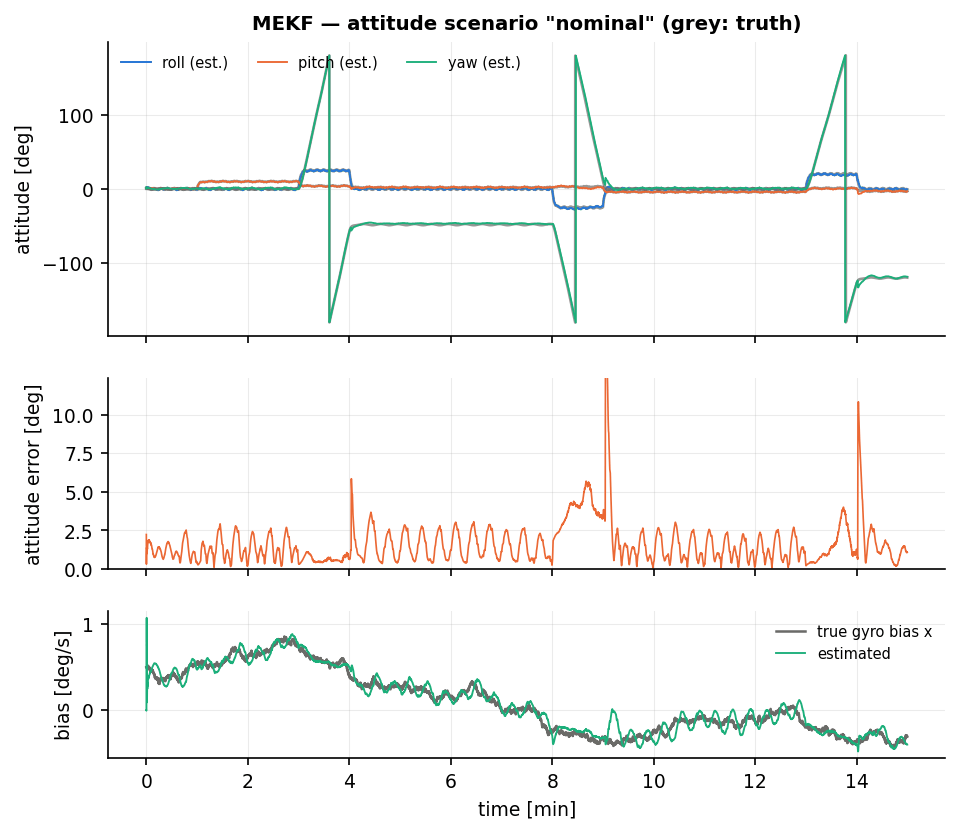
\includegraphics[width=\textwidth]{figures/imu_MEKF_nominal.png}
\caption{MEKF on the nominal mission: Euler angles, total angular error and the $x$-axis gyro-bias
estimate against truth.}
\end{figure}
\begin{figure}[H]\centering
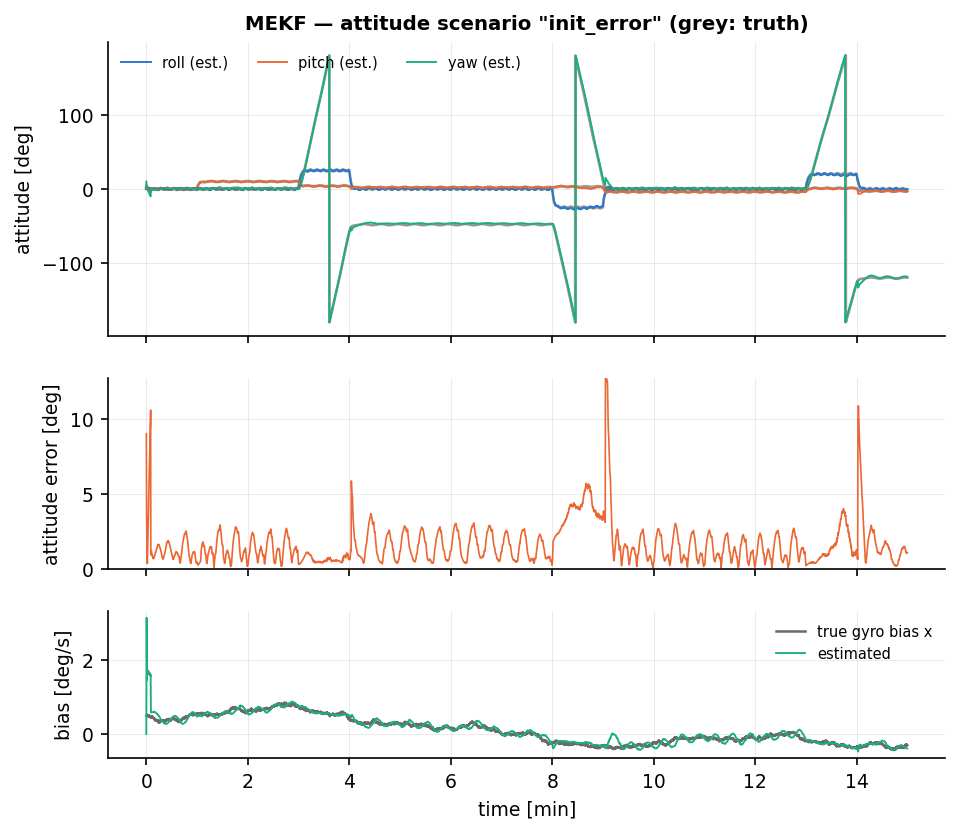
\includegraphics[width=\textwidth]{figures/imu_MEKF_init_error.png}
\caption{MEKF with a $46.6^\circ$ initial attitude error: the transient is over in
$\SI{0.24}{\second}$.}
\end{figure}

The registered MEKF is, with the invariant filter of the next chapter, the most uniform estimator
of the family: mission RMS $2.48/2.50/2.48/2.86/2.14/\SI{3.33}{\degree}$ across the six scenarios in
table order (\texttt{nominal}, \texttt{init\_error}, \texttt{gyro\_bias},
\texttt{mag\_disturbance}, \texttt{vibration}, \texttt{high\_dynamics}); on nominal roll $0.84$,
pitch $0.68$, yaw $\SI{2.23}{\degree}$, $\text{RMS}_{\text{ss}}=\SI{3.07}{\degree}$, peak
$\SI{15.1}{\degree}$, gyro-bias RMSE $\SI{0.17}{\degree\per\second}$ against a true
$\SI{1.03}{\degree\per\second}$, never lost, $t_{\text{conv}}=\SI{0}{\second}$,
$\SI{2.04}{\micro\second}$/step. The flatness of that row is the headline: the six-state filter is
essentially \emph{insensitive} to which scenario it is run on, which is what a correct covariance is
for. It is no longer the outright best --- \texttt{Mahony-Gated} (Chapter~\ref{ch:att-mahony})
reaches $\SI{2.14}{\degree}$ on nominal at one fifteenth of the cost --- but it is the only filter
apart from its invariant twin that is within $\SI{1}{\degree}$ of its own best on every scenario.

Table numbers are three-seed means; the ablations below are single-seed (seed~1) diagnostics, for
which the registered configuration scores $\SI{2.11}{\degree}$ on \texttt{nominal}.

\paragraph{Where the remaining $\SI{2.5}{\degree}$ lives.} Per phase on nominal (seed~1),
\[
1.30\;/\;1.50\;/\;1.15\;/\;1.74\;/\;4.53\;/\;1.91\;/\;2.69\;/\;1.86\ \SI{}{\degree}
\]
for take-off / climb / turn\,1 / cruise / turn\,2 / descent / turn\,3 / final. Two floors, both
quantified independently of any filter:
\begin{itemize}[nosep]
\item \textbf{Hard iron.} The dataset applies an uncompensated body-frame offset
$\bm{b}_m$ with components $0.30$, $-0.15$ and $\SI{0.25}{\micro\tesla}$, i.e.
$\norm{\bm{b}_m}=\SI{0.42}{\micro\tesla}$, or $0.87\,\%$ of the field. (This is the residual of a
\emph{calibrated} compass; the development dataset used $\SI{1.375}{\micro\tesla}$.) Fed to an
\emph{exact} tilt-compensated
compass with the true attitude it alone produces $\SI{0.65}{\degree}$ RMS and $\SI{1.12}{\degree}$
peak of heading error, because the horizontal component of a $65^\circ$-dip field is only
$\SI{20.3}{\micro\tesla}$. No estimator in this family calibrates hard iron~\cite{gebreegziabher2006},
so $\approx\SI{0.65}{\degree}$ of the $\SI{2.23}{\degree}$ yaw RMS is structural; the rest is the
residual tilt error amplified by $\tan I=2.14$.
\item \textbf{Turn coasting.} During the $\SI{60}{\second}$ turns the accelerometer is edited out
and the attitude is carried by the gyro plus the magnetometer alone. At $25^\circ$ of bank the field
lies close to the body vertical (measured: $\bm{m}=[2.0,0.5,47.7]^\T\,\SI{}{\micro\tesla}$ at
$t=\SI{488}{\second}$), so the direction the magnetometer cannot observe --- rotation about the
field --- is close to the heading axis, and the heading is held by the gyro for up to a minute at a
time. The result is $1.15$/$4.53$/$\SI{2.69}{\degree}$ on the three turns, compared with
$42$/$36$/$\SI{35}{\degree}$ for the filters that trust the accelerometer throughout. The second
turn is the worst of the three because it is the longest one flown at constant bank.
\end{itemize}

\paragraph{Ablation of the measurement model.} All on \texttt{nominal}, seed~1:
\begin{center}
\begin{tabular}{@{}lr@{}}
\toprule
configuration & RMS [deg] \\
\midrule
registered & $2.11$ \\
constant $\bm{\Sigma}$ (\code{gate=false}) & $19.61$ \\
magnitude gate only, no manoeuvre bound ($V_{\text{ref}}=0$) & $19.25$ \\
gate + manoeuvre bound but no editing & $7.80$ \\
$\sigma_{a,\text{extra}}=0.1 / 0.5 / \SI{2.0}{\metre\per\second\squared}$ & $4.77 / 2.11 / 1.67$ \\
$\sigma_{m,\text{extra}}=0.3 / 1.5 / \SI{5.0}{\micro\tesla}$ & $2.09 / 2.11 / 2.24$ \\
$q_{\text{scale}}=0.25 / 1 / 4$ & $1.71 / 2.11 / 4.01$ \\
Joseph form off / second-order $\bm{\Phi}$ off & $2.11 / 2.11$ (bit-identical) \\
centripetal mean correction on ($V=45$) & $7.15$ \\
magnetometer disabled & $113.59$ \\
\bottomrule
\end{tabular}
\end{center}
Four readings. First, the magnitude gate on its own is worth \emph{nothing}
($19.25$ versus $19.61$): Remark~\ref{rem:mekf-turn} is not a theoretical point. Second, the
rate-driven bound plus editing is worth a factor of nine, and editing alone is worth
$7.80\to2.11$, i.e. a factor of $3.7$ --- inflating $\bm{\Sigma}$ is not the same as rejecting the
measurement. Third, the filter is now essentially insensitive to
$\sigma_{m,\text{extra}}$ on nominal ($2.09$--$\SI{2.24}{\degree}$ over a factor of 17), which is
what one expects once the hard iron has been calibrated down to $\SI{0.42}{\micro\tesla}$; the one
place it still matters is \texttt{init\_error}, where $\sigma_{m,\text{extra}}=\SI{0.3}{\micro\tesla}$
costs $\SI{4.78}{\degree}$ against $\SI{2.16}{}$, because an over-confident magnetometer pulls the
filter too hard during the initial transient. Fourth, and least expected: switching on the
centripetal \emph{mean} correction --- which is what rescues the fixed-gain filter of
Chapter~\ref{ch:att-complementary} --- makes the MEKF \emph{worse}, $7.15$ against
$\SI{2.11}{\degree}$, and quadruples the bias RMSE ($0.68$ against
$\SI{0.17}{\degree\per\second}$). The reason is structural: the correction
$\bm{f}-(\bm{\omega}_y-\hat{\bm{b}})\times\bm{v}_b$ makes the \emph{measurement} a function of the
\emph{state estimate}, so a bias error can be explained away as a tilt error and vice versa. The
filter loses bias observability, which is precisely the state the MEKF exists to estimate. A
covariance-carrying filter should widen $\bm{\Sigma}$, not modify $\bm{y}$.

\paragraph{Initial-error transient.} From $46.6^\circ$ of attitude error the MEKF is below $5^\circ$
in $\SI{0.17}{\second}$ (17 samples) and below $2^\circ$ in $\SI{0.61}{\second}$; the
$\SI{30}{\second}$ window RMS is $\SI{2.71}{\degree}$ against $\SI{1.32}{\degree}$ from a perfect
start. From $78.5^\circ$ it needs $\SI{2.67}{\second}$ and the window RMS rises to
$\SI{3.52}{\degree}$: the first-order expansion
\eqref{eq:mekf-dtheta}--\eqref{eq:mekf-H} is being pushed past its validity, and the filter spends
the first two seconds correcting in a slightly wrong direction. The cost is visible even in the
table: on \texttt{init\_error} the MEKF's $t_{\text{conv}}$ slips to $\SI{3}{\second}$ and its bias
RMSE to $\SI{0.25}{\degree\per\second}$, against $\SI{0}{\second}$ and $\SI{0.18}{}$ for the
invariant filter. That degradation is exactly what the invariant formulation of
Chapter~\ref{ch:att-iekf} removes.

\paragraph{Cross-scenario detail.} \texttt{vibration} is the \emph{best} scenario
($\SI{2.14}{\degree}$): the configured $\sigma_a$ rises from $0.05$ to
$\SI{1.05}{\metre\per\second\squared}$, the filter widens $\bm{\Sigma}_a$ accordingly and simply
averages more --- this is the textbook demonstration of what a covariance-weighted filter buys over
a fixed-gain one (Madgwick: $14.78$, Mahony: $\SI{18.28}{\degree}$ on the same data).
\texttt{mag\_disturbance} costs $\SI{0.38}{\degree}$, all of it in yaw ($2.23\to2.64$): the field
magnitude rises from $48$ to $\SI{54}{\micro\tesla}$, $e_m$ exceeds the editing threshold and the
magnetometer is dropped for the $\SI{20}{\second}$ of the anomaly, during which the heading is held
by the gyro (cruise-phase RMS $1.74\to\SI{3.06}{\degree}$, seed~1). \texttt{gyro\_bias} costs
$\SI{0.004}{\degree}$ and the bias RMSE only rises from $0.17$ to $\SI{0.19}{\degree\per\second}$.
\texttt{high\_dynamics} is the worst at $\SI{3.33}{\degree}$ with
$t_{\text{conv}}=\SI{222}{\second}$, because the tripled turbulence rates cross the manoeuvre
threshold more often and the accelerometer is edited out more of the time.

\section{Summary}
The MEKF is the reference solution and behaves like one: $\SI{2.5}{\degree}$ RMS, flat to within
$\SI{1.2}{\degree}$ across all six scenarios, $\SI{0.17}{\degree\per\second}$ of bias error, never
lost, $\SI{2.04}{\micro\second}$ and 608\,bytes. Use it whenever a covariance is wanted downstream,
whenever the sensor statistics change during the mission (\texttt{vibration} is
$\SI{2.1}{\degree}$ here against $\SI{18.3}{\degree}$ for the published fixed-gain filters), and
whenever the gyro bias matters. Note, though, that a $\SI{132}{\nano\second}$ nonlinear observer
with the same disturbance model (\texttt{Mahony-Gated}) beats it on \texttt{nominal}
($2.14$ against $2.48$) and \texttt{mag\_disturbance} ($2.31$ against $\SI{2.86}{\degree}$): the
covariance earns its keep on the four \emph{hard} scenarios --- \texttt{init\_error}
($2.50$ against $3.76$), \texttt{gyro\_bias} ($2.48$ against $2.74$), \texttt{vibration}
($2.14$ against $2.47$) and \texttt{high\_dynamics} ($3.33$ against $\SI{4.83}{\degree}$) --- and in
the uncertainty it reports, not in the nominal RMS. The two things
to get right are not in the Kalman equations at all: the per-sample to per-root-second conversion
\eqref{eq:mekf-units}, and a measurement-covariance model that can see a coordinated turn
(Remark~\ref{rem:mekf-turn}) and edit it out rather than average it in. Its one structural weakness
--- a first-order error expansion that degrades above $\approx60^\circ$ of initial error --- is the
subject of the next chapter.

% Copyright 2026 Sreeram Anil
% SPDX-License-Identifier: CC-BY-4.0
% =============================================================================
%  Right-invariant EKF on SO(3) x R^3 — attitude (AHRS) family
% =============================================================================
\chapter{Right-Invariant Extended Kalman Filter (InvariantEKF)}
\label{ch:att-iekf}

\section*{At a glance}
\begin{tabular}{@{}l>{\raggedright\arraybackslash}p{0.76\textwidth}@{}}
Family & attitude / AHRS \\
Header & \texttt{include/estkit/attitude/iekf\_attitude.hpp} \\
Registered name & \texttt{InvariantEKF} \\
State & $\hat{\bm{q}}\in S^3$, $\hat{\bm{b}}\in\real^3$; error
 $[\bm{\xi};\bm{\beta}]\in\real^6$, $\bm{\xi}$ in the NAV frame; $\mP\in\real^{6\times6}$ \\
Cost per step & $\approx2.9\times10^3$ MACs; $\SI{1.91}{\micro\second}$/step, 608\,bytes \\
Primary references & \cite{barrau2017iekf,barrau2018review,bonnabel2007,bonnabel2009} \\
\end{tabular}

\section{Motivation and aerospace relevance}
The MEKF of Chapter~\ref{ch:att-mekf} linearises the error dynamics about the current estimate. That
is a choice, not a necessity: the error itself can be defined in more than one way, and some
definitions have dynamics that are \emph{exactly} linear no matter how large the error or how
violent the trajectory. Barrau and Bonnabel~\cite{barrau2017iekf} characterised the systems for
which this happens --- \emph{group-affine} systems on matrix Lie groups --- and showed that for them
the invariant error obeys a \emph{log-linear} differential equation whose transition matrix is
independent of the state. The consequences are two, and both are visible in the benchmark: the
filter cannot manufacture false observability from a wrong estimate, and its domain of attraction is
much larger than an ordinary EKF's.

The attitude problem is the simplest non-trivial instance. $\dot{\bm{R}}=\bm{R}[\bm{\omega}]_\times$
is equivariant under left translations $\bm{R}\mapsto\bm{R}_0\bm{R}$ --- a change of navigation frame
--- so the natural error is the \emph{right}-invariant one, and with the same input applied to truth
and estimate it is exactly conserved. That fact is one line of algebra, \eqref{eq:iekf-eta0} below,
and it replaces the MEKF's $\exp(-[\hat{\bm{\omega}}]_\times\dt)$ by the identity.

Invariant filtering is now standard in aided inertial navigation (the $SE_2(3)$ formulation of
IMU/GNSS fusion, legged-robot state estimation, visual-inertial odometry) and in spacecraft attitude
work; the attitude-only case treated here is the pedagogical core of it.

\section{Problem statement and assumptions}
The models are exactly those of Chapter~\ref{ch:att-mekf}, \eqref{eq:mekf-gyro}--\eqref{eq:mekf-meas},
and the measurement-covariance policy of \S\ref{sec:mekf-R} is reused verbatim, so that any
difference in the benchmark is attributable to the error parametrisation and to nothing else.

\begin{definition}[Invariant errors]
For $\bm{R},\hat{\bm{R}}\in SO(3)$ the \emph{right}-invariant error is
$\bm{\eta}_R=\hat{\bm{R}}\bm{R}^\T$ (invariant under $\bm{R}\mapsto\bm{R}_0\bm{R}$,
$\hat{\bm{R}}\mapsto\bm{R}_0\hat{\bm{R}}$ up to conjugation, and a NAV-frame object) and the
\emph{left}-invariant error is $\bm{\eta}_L=\bm{R}^\T\hat{\bm{R}}$ (a BODY-frame object). The MEKF's
$\delta\bm{\theta}$ is the logarithm of $\bm{\eta}_L^{-1}$.
\end{definition}

\section{Derivation}

\subsection{Why the right-invariant error is the right one here}
Assume for a moment a perfect gyro, $\hat{\bm{\omega}}=\bm{\omega}$. Then
$\dot{\bm{R}}=\bm{R}[\bm{\omega}]_\times$ and $\dot{\hat{\bm{R}}}=\hat{\bm{R}}[\bm{\omega}]_\times$,
so, using $\dot{(\bm{R}^\T)}=-[\bm{\omega}]_\times\bm{R}^\T$,
\begin{equation}
\dot{\bm{\eta}}_R = \dot{\hat{\bm{R}}}\bm{R}^\T + \hat{\bm{R}}\dot{(\bm{R}^\T)}
 = \hat{\bm{R}}[\bm{\omega}]_\times\bm{R}^\T - \hat{\bm{R}}[\bm{\omega}]_\times\bm{R}^\T = \bm{0}.
\label{eq:iekf-eta0}
\end{equation}
The right-invariant error is \emph{exactly constant}: no linearisation, no dependence on
$\bm{\omega}$, no dependence on how large the error is. This is the log-linear property of
Barrau and Bonnabel~\cite[Thm.~1]{barrau2017iekf} in its simplest form; the attitude block of the
error-propagation matrix is the identity. Contrast the MEKF, whose body-frame error obeys
$\dot{\delta\bm{\theta}}=-[\hat{\bm{\omega}}]_\times\delta\bm{\theta}+\dots$ --- correct only to
first order, and driven by the estimated (hence possibly wrong) rate.

Note that the \emph{left}-invariant error would \emph{not} be conserved here, because the dynamics
are right-multiplicative; the choice of error must match the symmetry of the dynamics, and the
symmetry is fixed by the fact that $\bm{\omega}$ is a body rate.

\subsection{The imperfect IEKF: adding the gyro bias}
A bias breaks the picture, because $\bm{b}$ does not live in $SO(3)$ and the augmented system is no
longer group-affine; this is the ``imperfect IEKF'' of \cite[Sec.~V]{barrau2017iekf}. Repeating
\eqref{eq:iekf-eta0} with $\hat{\bm{\omega}}=\bm{\omega}_y-\hat{\bm{b}}$,
$\bm{\omega}=\bm{\omega}_y-\bm{b}-\bm{n}_v$ and $\bm{\beta}=\bm{b}-\hat{\bm{b}}$,
\begin{equation}
\dot{\bm{\eta}}_R = \hat{\bm{R}}\big[\hat{\bm{\omega}}-\bm{\omega}\big]_\times\bm{R}^\T
 = \hat{\bm{R}}\big[\bm{\beta}+\bm{n}_v\big]_\times\hat{\bm{R}}^\T\,\bm{\eta}_R
 = \big[\hat{\bm{R}}(\bm{\beta}+\bm{n}_v)\big]_\times\,\bm{\eta}_R ,
\label{eq:iekf-etadot}
\end{equation}
using $\bm{A}[\bm{v}]_\times\bm{A}^\T=[\bm{A}\bm{v}]_\times$ for $\bm{A}\in SO(3)$. Writing
$\bm{\eta}_R=\exp([\bm{\xi}]_\times)$ with $\bm{\xi}\in\real^3$ a \emph{navigation-frame} rotation
vector, \eqref{eq:iekf-etadot} gives to first order in $\bm{\xi}$
\begin{equation}
\dot{\bm{\xi}} = \hat{\bm{R}}\big(\bm{\beta}+\bm{n}_v\big),
\qquad
\dot{\bm{\beta}} = \bm{n}_u ,
\label{eq:iekf-err}
\end{equation}
so
\begin{equation}
\mF = \begin{bmatrix}\bm{0} & \hat{\bm{R}}\\ \bm{0}&\bm{0}\end{bmatrix},
\qquad
\bm{\Phi}=\exp(\mF\dt)=\begin{bmatrix}\bm{I} & \hat{\bm{R}}\dt\\ \bm{0}&\bm{I}\end{bmatrix}
\quad\text{exactly, since } \mF^2=\bm{0}.
\label{eq:iekf-Phi}
\end{equation}
Three things are worth saying about \eqref{eq:iekf-Phi}. \emph{(i)} The attitude block is
\emph{exactly} the identity --- there is no $\exp(-[\hat{\bm{\omega}}]_\times\dt)$ and therefore no
trajectory dependence whatsoever in the attitude error propagation. \emph{(ii)} The only state
dependence left is the rotation $\hat{\bm{R}}$ in the coupling block, which merely expresses that
the bias is a body-frame quantity while $\bm{\xi}$ is a navigation-frame one. \emph{(iii)} The
matrix exponential is exact, not truncated, because $\mF$ is nilpotent.

The discrete process noise follows from van Loan~\cite{vanloan1978} as in \eqref{eq:mekf-Q};
$\hat{\bm{R}}\hat{\bm{R}}^\T=\bm{I}$ removes the rotation from the diagonal blocks and leaves it in
the cross term:
\begin{equation}
\mQ_d=\begin{bmatrix}
 \big(\sigma_v^2\dt+\tfrac13\sigma_u^2\dt^3\big)\bm{I} & \tfrac12\sigma_u^2\dt^2\,\hat{\bm{R}}\\[2pt]
 \tfrac12\sigma_u^2\dt^2\,\hat{\bm{R}}^\T & \sigma_u^2\dt\,\bm{I}\end{bmatrix} .
\label{eq:iekf-Q}
\end{equation}
The sign of the cross block is opposite to the MEKF's \eqref{eq:mekf-Q}, because $\mF_{12}$ is
$+\hat{\bm{R}}$ here and $-\bm{I}$ there.

\subsection{Right-invariant observations and the invariant innovation}
Gravity and the magnetic field are observed as $\bm{y}=\bm{R}^\T\bm{r}+\bm{n}$ with $\bm{r}$ a
\emph{known navigation} vector. In the language of \cite{barrau2017iekf} these are
\emph{right-invariant} observations: they are of the form $\bm{y}=\chi^{-1}\bm{r}$ and are therefore
compatible with the right-invariant error. The invariant innovation is formed by carrying the
measurement into the navigation frame,
\begin{equation}
\bm{z} = \hat{\bm{R}}\bm{y} - \bm{r}
 = \bm{\eta}_R\bm{r} - \bm{r} + \hat{\bm{R}}\bm{n}
 = \bm{\xi}\times\bm{r} + \hat{\bm{R}}\bm{n} + O(\norm{\bm{\xi}}^2)
 = -[\bm{r}]_\times\bm{\xi} + \hat{\bm{R}}\bm{n} + O(\norm{\bm{\xi}}^2),
\label{eq:iekf-z}
\end{equation}
hence
\begin{equation}
\mH = \big[\,-[\bm{r}]_\times\quad \bm{0}_{3\times3}\,\big],
\qquad
\operatorname{cov}\!\big(\hat{\bm{R}}\bm{n}\big)=\hat{\bm{R}}\,\sigma^2\bm{I}\,\hat{\bm{R}}^\T=\sigma^2\bm{I} .
\label{eq:iekf-H}
\end{equation}
\begin{remark}[The state has disappeared from the filter gain]
$\mH$ in \eqref{eq:iekf-H} depends only on the \emph{known} reference $\bm{r}$ --- not on
$\hat{\bm{q}}$, not on the trajectory --- and for isotropic sensor noise neither does the
measurement covariance. Combined with $\bm{\Phi}_{11}=\bm{I}$, this means the entire covariance
recursion of the attitude block is deterministic: $\mP$, $\mS$ and $\mK$ evolve along a
trajectory-independent path. An ordinary EKF's $\mH=[\hat{\bm{R}}^\T\bm{r}]_\times$ is evaluated at
the estimate, so a wrong estimate produces a wrong gain and, worse, a covariance that reflects the
observability of a system the vehicle is not on --- the ``false observability'' that makes EKFs
inconsistent after a large heading error. The invariant filter cannot do this.
\end{remark}

\subsection{Update and reset}
The Kalman update is the usual one on $[\bm{\xi};\bm{\beta}]$ with the stacked accelerometer and
magnetometer blocks, in Joseph form. Since $\bm{\eta}_R=\hat{\bm{R}}\bm{R}^\T=\exp([\bm{\xi}]_\times)$
implies $\bm{R}=\exp(-[\bm{\xi}]_\times)\hat{\bm{R}}$, the correction is a \emph{left}
(navigation-frame) multiplication,
\begin{equation}
\hat{\bm{q}}\leftarrow \exp\!\big(-\bm{\xi}^+\big)\otimes\hat{\bm{q}},
\qquad
\hat{\bm{b}}\leftarrow \hat{\bm{b}}+\bm{\beta}^+ ,
\label{eq:iekf-reset}
\end{equation}
where the MEKF's reset \eqref{eq:mekf-reset} is a right multiplication. That single difference ---
which side the correction is applied on, and correspondingly in which frame the error is
expressed --- is the whole of the invariant EKF.

A second-order reset transform for the cross-covariance (the bias error is body-referenced and
$\hat{\bm{R}}$ has just changed) is $O(\norm{\bm{\xi}^+}^2)$ and is omitted, as in
\cite{barrau2018review}.

\section{Algorithm}
\begin{algorithm}[H]
\caption{Right-invariant EKF --- one sampling period}
\begin{algorithmic}[1]
\Require $\hat{\bm{q}},\hat{\bm{b}},\mP$; $\bm{\omega}_y,\bm{f},\bm{m}$
\State $\hat{\bm{\omega}}\gets\bm{\omega}_y-\hat{\bm{b}}$;\;
       $\hat{\bm{q}}\gets\hat{\bm{q}}\otimes\exp(\hat{\bm{\omega}}\dt)$, normalise;\;
       $\hat{\bm{R}}\gets\bm{R}(\hat{\bm{q}})$
\State $\bm{\Phi}\gets\big[\begin{smallmatrix}\bm{I}&\hat{\bm{R}}\dt\\ \bm{0}&\bm{I}\end{smallmatrix}\big]$;\;
       $\mQ_d\gets$ \eqref{eq:iekf-Q};\; $\mP\gets\bm{\Phi}\mP\bm{\Phi}^\T+\mQ_d$; symmetrise
\State $\bm{z}\gets\big[\hat{\bm{R}}\bm{f}-\bm{r}_a;\ \hat{\bm{R}}\bm{m}-\bm{r}_m\big]$
       \Comment{invariant innovation, NAV frame}
\State $\mH\gets\big[\begin{smallmatrix}-[\bm{r}_a]_\times&\bm{0}\\ -[\bm{r}_m]_\times&\bm{0}\end{smallmatrix}\big]$
       \Comment{constant matrices}
\State $\bm{\Sigma}\gets$ \eqref{eq:mekf-R}--\eqref{eq:mekf-sx} with editing
\State $\mK\gets\mP\mH^\T(\mH\mP\mH^\T+\bm{\Sigma})\inv$;\;
       $[\bm{\xi}^+;\bm{\beta}^+]\gets\mK\bm{z}$
\State $\mP\gets(\mI-\mK\mH)\mP(\mI-\mK\mH)^\T+\mK\bm{\Sigma}\mK^\T$; symmetrise
\State $\hat{\bm{q}}\gets\exp(-\bm{\xi}^+)\otimes\hat{\bm{q}}$, normalise;\;
       $\hat{\bm{b}}\gets\operatorname{clamp}(\hat{\bm{b}}+\bm{\beta}^+)$
\Ensure $\hat{\bm{q}},\hat{\bm{b}},\mP$
\end{algorithmic}
\end{algorithm}

\section{Application to the benchmark flight}
Identical to the MEKF, deliberately: $\mP_0=\diag((30^\circ)^2\bm{I},(\SI{3}{\degree\per\second})^2\bm{I})$,
$\sigma_v,\sigma_u$ from the configuration through \eqref{eq:mekf-units},
$\sigma_{a,\text{extra}}=\SI{0.5}{\metre\per\second\squared}$,
$\sigma_{m,\text{extra}}=\SI{1.5}{\micro\tesla}$, $V_{\text{ref}}=\SI{45}{\metre\per\second}$,
$\varpi=\SI{0.02}{\radian\per\second}$, editing at $\SI{1}{\metre\per\second\squared}$ and
$\SI{3}{\micro\tesla}$, Joseph form. Nothing was re-tuned for this filter, so the comparison in the
results is a clean A/B on the error parametrisation.

\section{Implementation notes}
The cost is the same $\approx2.9\times10^3$ multiply--adds as the MEKF, and in fact measurably
lower in practice ($\SI{1.91}{\micro\second}$/step against $\SI{2.04}{}$, a $6\,\%$ saving) because
$\bm{\Phi}$ is assembled from a rotation matrix that is needed anyway and requires no
$\sin/\cos$ evaluation --- the closed-form $\bm{\Phi}_{11},\bm{\Phi}_{12}$ of the MEKF,
\eqref{eq:mekf-phi11}--\eqref{eq:mekf-phi12}, are gone. \code{sizeof} is 608\,bytes, identical.

A production implementation can exploit more: $\mH$ in \eqref{eq:iekf-H} is a pair of \emph{constant}
skew matrices, so $\mH\mP\mH^\T$ and $\mP\mH^\T$ are cross products rather than general matrix
products, and if $\bm{\Sigma}$ were constant the whole gain sequence could be precomputed offline
(it is not here, because of the adaptive $\bm{\Sigma}$ of \S\ref{sec:mekf-R}).

Numerical hygiene: as for the MEKF --- symmetrisation after both updates, Joseph form, finiteness
checks on $\mK$ and on the correction, quaternion renormalisation after the reset, bias clamped to
$\pm\SI{15}{\degree\per\second}$. \code{Quat::exp} falls back to its first-order form below
$10^{-9}$\,rad. The single-precision build reproduces the double-precision mission RMS to four digits.

\section{Benchmark results}
% Copyright 2026 Sreeram Anil
% SPDX-License-Identifier: CC-BY-4.0
\begin{table}[H]\centering\footnotesize\setlength{\tabcolsep}{3.5pt}\caption{InvariantEKF: attitude benchmark (mean over seeds; all angles in degrees; $t_\mathrm{conv}$: first time the attitude error stays below 2$^\circ$ for 30\,s; bias RMSE in deg/s; 608 bytes of state).}\label{tab:imu_InvariantEKF}
\begin{tabular}{lrrrrrrrrcr}\toprule scenario & RMS & roll & pitch & yaw & max & RMS$_\mathrm{ss}$ & $t_\mathrm{conv}$ [s] & bias RMSE & lost & ns/step \\ \midrule
nominal & 2.49 & 0.84 & 0.68 & 2.24 & 15.1 & 3.08 & 0 & 0.17 & no & 1910 \\
init\_error & 2.49 & 0.84 & 0.68 & 2.24 & 15.1 & 3.08 & 0 & 0.18 & no & 1910 \\
gyro\_bias & 2.49 & 0.84 & 0.68 & 2.24 & 15.1 & 3.08 & 2 & 0.19 & no & 1934 \\
mag\_disturbance & 2.88 & 0.85 & 0.68 & 2.66 & 15.9 & 3.08 & 0 & 0.19 & no & 1901 \\
vibration & 2.14 & 0.71 & 0.57 & 1.93 & 16.6 & 2.52 & 11 & 0.15 & no & 1906 \\
high\_dynamics & 3.30 & 1.15 & 0.76 & 3.02 & 12.7 & 3.90 & 222 & 0.20 & no & 1909 \\
\bottomrule\end{tabular}\end{table}

\begin{figure}[H]\centering
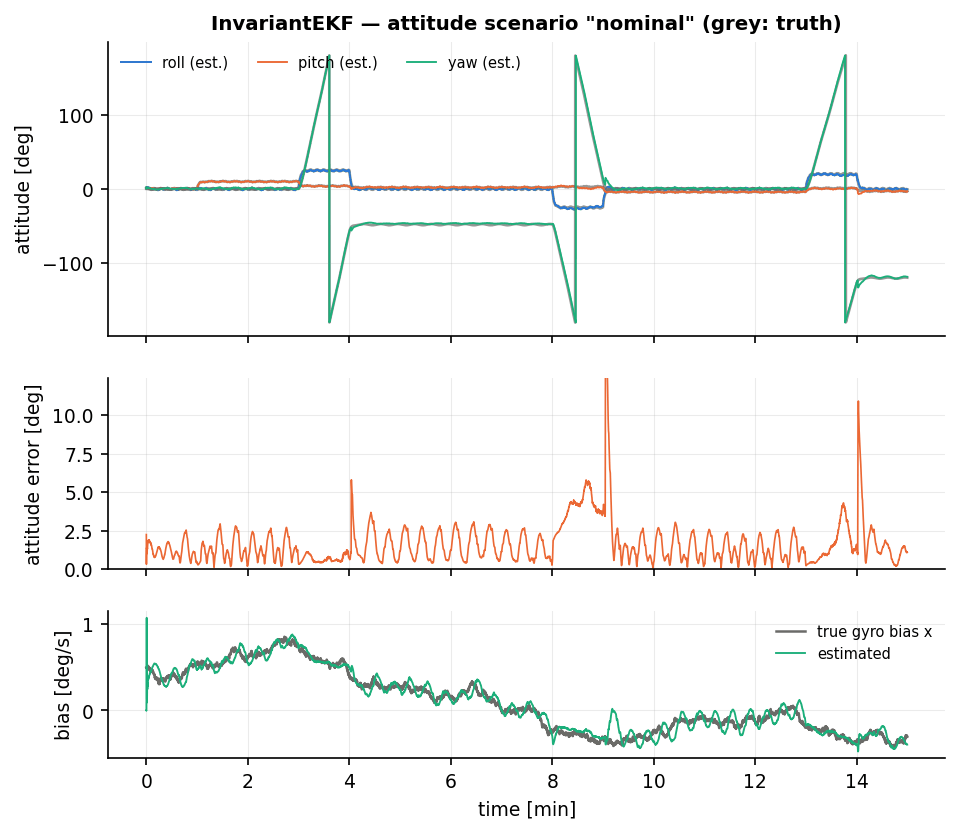
\includegraphics[width=\textwidth]{figures/imu_InvariantEKF_nominal.png}
\caption{Invariant EKF on the nominal mission.}
\end{figure}
\begin{figure}[H]\centering
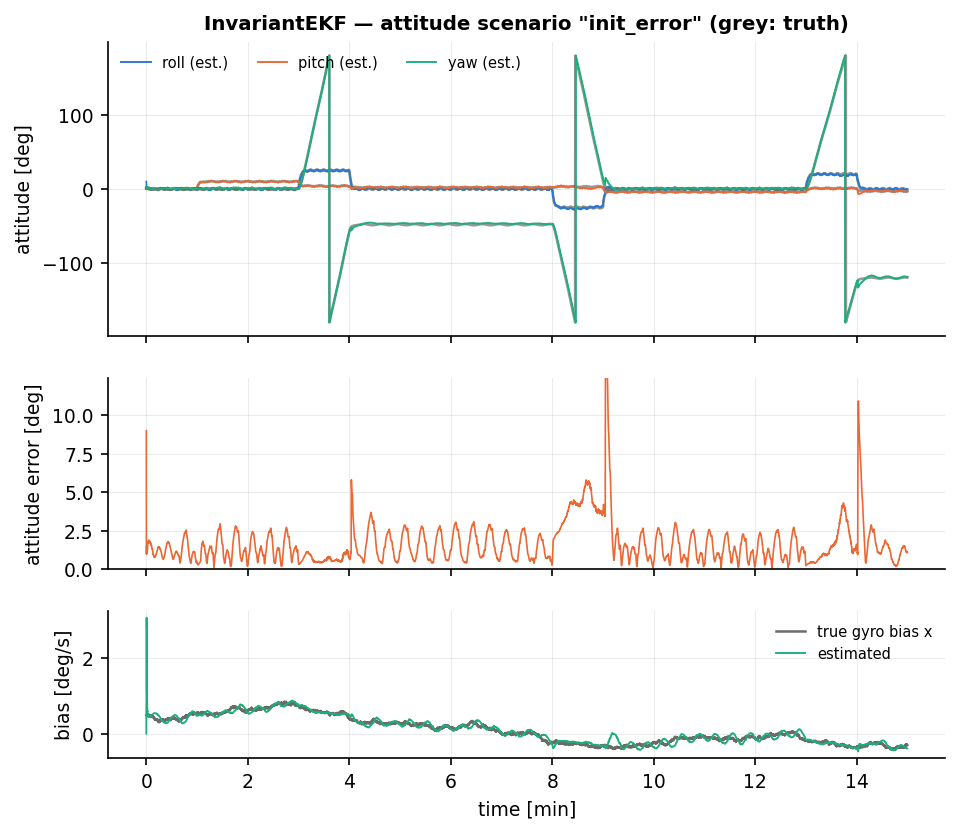
\includegraphics[width=\textwidth]{figures/imu_InvariantEKF_init_error.png}
\caption{Invariant EKF with a $46.6^\circ$ initial attitude error: the transient lasts one sample.}
\end{figure}

In steady state the two six-state filters are indistinguishable, as they should be --- at
$\norm{\bm{\xi}}<1^\circ$ the two linearisations agree to second order. Mission RMS across the six
scenarios in table order is $2.49/2.49/2.49/2.88/2.14/\SI{3.30}{\degree}$, against the MEKF's
$2.48/2.50/2.48/2.86/2.14/\SI{3.33}{\degree}$; on nominal roll $0.84$, pitch $0.68$, yaw
$\SI{2.24}{\degree}$, $\text{RMS}_{\text{ss}}=\SI{3.08}{\degree}$, peak $\SI{15.1}{\degree}$, bias
RMSE $\SI{0.17}{\degree\per\second}$, never lost, and the cost is
$\SI{1.91}{\micro\second}$/step. Per phase on nominal (seed~1),
\[
1.30\;/\;1.50\;/\;1.16\;/\;1.74\;/\;4.63\;/\;1.91\;/\;2.78\;/\;1.86\ \SI{}{\degree},
\]
i.e. within $\SI{0.1}{\degree}$ of the MEKF in every phase. The invariant formulation is \emph{not} a free accuracy improvement in the regime the
mission spends its time in, and saying otherwise would be dishonest.

Two differences do survive into the three-seed table, both small and both in the predicted
direction. On \texttt{init\_error} the invariant filter reports $t_{\text{conv}}=\SI{0}{\second}$
and a bias RMSE of $\SI{0.18}{\degree\per\second}$ --- identical to its own nominal row --- while the
MEKF slips to $\SI{3}{\second}$ and $\SI{0.25}{\degree\per\second}$: the MEKF's initial transient
leaks into its bias estimate and the invariant filter's does not. On \texttt{high\_dynamics}, where
the angular rates are tripled and the MEKF's $\exp(-[\hat{\bm{\omega}}]_\times\dt)$ has the most work
to do, the invariant filter is marginally better ($3.30$ against $\SI{3.33}{\degree}$).

\paragraph{Where it does pay: large initial error.} The benchmark's \texttt{init\_error} scenario is
too gentle to separate the two in mission RMS (the transient lasts under a second out of
$\SI{900}{\second}$). Measured directly, starting the two filters from a deliberately wrong attitude
on the nominal data (seed~1) and recording the time to bring the total angular error below a
threshold:
\begin{center}
\begin{tabular}{@{}lrrrrr@{}}
\toprule
initial error & \multicolumn{2}{c}{$t(<5^\circ)$ [s]} & \multicolumn{2}{c}{$t(<2^\circ)$ [s]} & RMS over first $\SI{30}{\second}$ \\
\cmidrule(lr){2-3}\cmidrule(lr){4-5}\cmidrule(lr){6-6}
 & MEKF & IEKF & MEKF & IEKF & MEKF\,/\,IEKF [deg] \\
\midrule
$0^\circ$      & $0.00$ & $0.00$ & $0.01$ & $0.01$ & $1.32$\,/\,$1.32$ \\
$46.6^\circ$   & $0.17$ & $\bm{0.01}$ & $0.61$ & $\bm{0.04}$ & $2.71$\,/\,$\bm{1.33}$ \\
$78.5^\circ$   & $2.67$ & $\bm{0.04}$ & $3.69$ & $\bm{1.15}$ & $3.52$\,/\,$\bm{1.57}$ \\
$90.0^\circ$   & $0.08$ & $0.07$ & $1.57$ & $\bm{0.16}$ & $1.59$\,/\,$1.54$ \\
\bottomrule
\end{tabular}
\end{center}
From $46.6^\circ$ the invariant filter is inside $5^\circ$ after \emph{one sample}
($\SI{0.01}{\second}$) where the MEKF needs 17; from $78.5^\circ$ the ratio is 67. The reason is
exactly \eqref{eq:iekf-eta0} and \eqref{eq:iekf-H}: the propagation of the attitude error involves
no approximation at all, and the measurement Jacobian is evaluated at the known reference rather
than at the (badly wrong) estimate, so the first gain is the \emph{correct} gain rather than one
computed for an attitude the vehicle is nowhere near. The first-$\SI{30}{\second}$ RMS, a fairer
statistic than a threshold crossing, is $\SI{1.57}{\degree}$ against $\SI{3.52}{\degree}$ at
$78.5^\circ$ --- and the invariant filter's $\SI{1.33}{\degree}$ at $46.6^\circ$ is the same as its
own value from a \emph{perfect} start, which is as strong a statement of the log-linear property as
this benchmark can make.

\paragraph{Where it does not pay.} With a deliberately over-loose bias prior,
$\mP_{0,bb}=(\SI{10}{\degree\per\second})^2\bm{I}$, the invariant filter is \emph{worse} than the
MEKF on two scenarios ($9.21$ versus $\SI{8.77}{\degree}$ on \texttt{init\_error}, and $9.95$ versus
$\SI{1.84}{\degree}$ on \texttt{vibration}); at the registered $\SI{3}{\degree\per\second}$ the two
agree to $\SI{0.03}{\degree}$. The mechanism is the one the theory warns about: the bias is
\emph{not} part of the group, so \eqref{eq:iekf-Phi} is only ``imperfectly'' invariant, and the
cross-block $\hat{\bm{R}}\dt$ maps a body-referenced bias error into a navigation-referenced
attitude error through a rotation that itself turns by $312^\circ$ during the mission. A large
initial bias uncertainty is therefore smeared over navigation directions in a way the MEKF's
constant $-\bm{I}\dt$ coupling avoids. The invariance argument buys exactness in the attitude block
and nothing in the bias block, and it is honest to say so.

\paragraph{Everything else is shared.} Because the two filters use the same $\bm{\Sigma}$ policy,
the ablations of Chapter~\ref{ch:att-mekf} carry over unchanged: with editing disabled the invariant
filter gives $\SI{7.81}{\degree}$ against the MEKF's $\SI{7.80}{\degree}$; with no manoeuvre bound
both are near $\SI{19.3}{\degree}$. \texttt{vibration} is again the best scenario
($\SI{2.14}{\degree}$) and \texttt{high\_dynamics} the worst ($\SI{3.30}{\degree}$). The
$\SI{0.65}{\degree}$ hard-iron heading floor and the $\tan I=2.14$ dip amplification quantified in
Chapter~\ref{ch:att-mekf} apply identically here.

\section{Summary}
The right-invariant EKF is the MEKF with the attitude error moved from the body frame to the
navigation frame. One line of algebra, \eqref{eq:iekf-eta0}, then makes the attitude-error
propagation exact and the measurement Jacobian \eqref{eq:iekf-H} state-independent, at identical
cost --- slightly cheaper here, since the closed-form transition matrix is replaced by a rotation
that was needed anyway. Use it whenever the initial attitude may be badly wrong (coarse alignment,
post-fault recovery, in-flight re-initialisation), whenever consistency of the reported covariance
matters, or whenever the vehicle is highly dynamic: from a $78.5^\circ$ initial error it converges
$67$ times faster than the MEKF and more than halves the first-$\SI{30}{\second}$ RMS. Do not expect it to
improve steady-state accuracy --- here it is within $\SI{0.03}{\degree}$ of the MEKF on every
scenario, and both are beaten on \texttt{nominal} by a $\SI{132}{\nano\second}$ gated Mahony filter
(Chapter~\ref{ch:att-mahony}) --- and do not expect the invariance to extend to the bias, which is
not a group element: with a very loose bias prior the invariant filter is the more fragile of the
two.

% Copyright 2026 Sreeram Anil
% SPDX-License-Identifier: CC-BY-4.0
% =============================================================================
%  TRIAD — single-frame attitude determination, attitude (AHRS) family
% =============================================================================
\chapter{Single-Frame Attitude Determination: TRIAD}
\label{ch:att-triad}

\section*{At a glance}
\begin{tabular}{@{}l>{\raggedright\arraybackslash}p{0.76\textwidth}@{}}
Family & attitude / AHRS (memory-less baseline) \\
Header & \texttt{include/estkit/attitude/triad\_quest.hpp} \\
Registered name & \texttt{TRIAD} \\
State & none: $\bm{q}_k$ is a function of $(\bm{f}_k,\bm{m}_k)$ alone \\
Cost per step & $\approx120$ flops, one \code{sqrt};
  $\SI{129}{\nano\second}$/step, 120\,bytes \\
Primary references & \cite{black1964,shusteroh1981,markleymortari2000} \\
\end{tabular}

\section{Motivation and aerospace relevance}
Every estimator in this family except this one and its sibling (Chapter~\ref{ch:att-quest}) carries
state. TRIAD carries none: it solves for the attitude from the two vector observations available at
the current instant and throws the answer away. Black's 1964 note~\cite{black1964} --- two pages,
written for the Transit navigation satellites --- is the oldest attitude algorithm still in routine
use, and it is the one an AHRS falls back to for coarse alignment, for sanity-checking a filter, and
for initialising one.

Its role in this benchmark is diagnostic. Because it has no memory, no tuning and no dynamics
model, its error \emph{is} the instantaneous inconsistency of the sensor pair: it measures the
quality of the measurements, not the quality of an algorithm. Every filtered estimator in the family
should be read against it --- what a filter achieves \emph{below} the TRIAD error is exactly what
its memory bought, and where a filter is no better than TRIAD, its memory is not being used.

\section{Problem statement and assumptions}
Given $m=2$ pairs of unit vectors, $\bm{b}_i$ in the BODY frame and $\bm{r}_i$ in the NAV frame,
related by an unknown rotation,
\begin{equation}
\bm{b}_i \;=\; \bm{R}^\T\bm{r}_i + \text{noise},\qquad i=1,2,
\label{eq:tr-obs}
\end{equation}
find $\bm{R}\in SO(3)$. Here $\bm{r}_1=[0,0,-1]^\T$ with $\bm{b}_1=\bm{f}/\norm{\bm{f}}$ (the NED
reference of a normalised specific-force measurement) and
$\bm{r}_2=\bm{m}_{\text{nav}}/\norm{\bm{m}_{\text{nav}}}$ with $\bm{b}_2=\bm{m}/\norm{\bm{m}}$.

Two observations are the minimum: one unit vector fixes two degrees of freedom and leaves the
rotation about itself free. Two are also, in general, one too many --- \eqref{eq:tr-obs} is
over-determined (four independent constraints for three unknowns) and generally inconsistent, since
the measured angle between $\bm{b}_1$ and $\bm{b}_2$ will not equal the reference angle between
$\bm{r}_1$ and $\bm{r}_2$. TRIAD resolves the inconsistency by fiat: it satisfies one observation
\emph{exactly} and uses the other only for the remaining degree of freedom. Which one is
``primary'' is the method's only design choice.

\section{Derivation}
Let $\bm{b}_p,\bm{r}_p$ be the primary pair and $\bm{b}_s,\bm{r}_s$ the secondary pair. Build two
right-handed orthonormal triads, one from the body observations and one from the references:
\begin{equation}
\bm{t}_1 = \bm{b}_p,\quad
\bm{t}_2 = \frac{\bm{b}_p\times\bm{b}_s}{\norm{\bm{b}_p\times\bm{b}_s}},\quad
\bm{t}_3 = \bm{t}_1\times\bm{t}_2;
\qquad
\bm{u}_1 = \bm{r}_p,\quad
\bm{u}_2 = \frac{\bm{r}_p\times\bm{r}_s}{\norm{\bm{r}_p\times\bm{r}_s}},\quad
\bm{u}_3 = \bm{u}_1\times\bm{u}_2 .
\label{eq:tr-triads}
\end{equation}
Both $[\bm{t}_1\,\bm{t}_2\,\bm{t}_3]$ and $[\bm{u}_1\,\bm{u}_2\,\bm{u}_3]$ are orthogonal matrices
by construction, so
\begin{equation}
\bm{R} \;=\; [\bm{u}_1\,\bm{u}_2\,\bm{u}_3]\,[\bm{t}_1\,\bm{t}_2\,\bm{t}_3]^\T
 \;=\; \sum_{i=1}^{3}\bm{u}_i\bm{t}_i^\T \;\in\;SO(3)
\label{eq:tr-R}
\end{equation}
is a rotation, and $\bm{R}\bm{b}_p=\bm{u}_1=\bm{r}_p$ exactly: the primary observation is satisfied
without residual, while the secondary contributes only through the plane it spans with the primary
(its component along $\bm{b}_p$ is discarded). \eqref{eq:tr-R} needs no iteration, no
decomposition, and no trigonometry.

The rotation matrix is converted to a quaternion by Shepperd's algorithm~\cite{shepperd1978}, which
selects the largest of $\{\tr\bm{R},R_{11},R_{22},R_{33}\}$ so that the divisor is never below
$\tfrac12$ and the relative error is bounded for any rotation, including the $180^\circ$ case where
the naive trace formula loses all precision. The mission yaw passes through $\pm180^\circ$ twice, so
this is not a hypothetical.

\subsection{Error behaviour and the degeneracy}
Perturb the secondary observation by an angle $\varepsilon_s$. Its component perpendicular to
$\bm{b}_p$ is what determines $\bm{t}_2$, so the resulting attitude error about $\bm{b}_p$ is
\begin{equation}
\delta\vartheta \;\approx\; \frac{\varepsilon_s}{\sin\gamma},
\qquad \gamma = \angle(\bm{b}_p,\bm{b}_s),
\label{eq:tr-amplify}
\end{equation}
while a perturbation $\varepsilon_p$ of the primary passes through unattenuated. Two consequences:
\begin{itemize}[nosep]
\item TRIAD is \emph{asymmetric}. All of the primary sensor's error enters the answer; only the
perpendicular part of the secondary's does, amplified by $1/\sin\gamma$. Shuster and
Oh~\cite{shusteroh1981} show that TRIAD is the limit of the optimal weighted solution
(Chapter~\ref{ch:att-quest}) as the primary weight tends to infinity, which makes it optimal only if
the primary sensor really is much better than the secondary.
\item TRIAD is \emph{ill-conditioned when the observations are nearly collinear or
anti-collinear}. At $\gamma\to0$ or $\pi$ the cross product in \eqref{eq:tr-triads} vanishes and
$\bm{t}_2$ is defined by noise alone. This is not an academic concern in an AHRS at high magnetic
latitude: see the results.
\end{itemize}

\section{Algorithm}
\begin{algorithm}[H]
\caption{TRIAD --- one sampling period (the gyroscope is ignored)}
\begin{algorithmic}[1]
\Require $\bm{f},\bm{m}$; references $\bm{r}_1=[0,0,-1]^\T$, $\bm{r}_2=\hat{\bm{m}}_{\text{nav}}$
\State \textbf{if} $\norm{\bm{f}}$ or $\norm{\bm{m}}$ is negligible \textbf{then return} previous $\bm{q}$
\State $\bm{b}_1\gets\bm{f}/\norm{\bm{f}}$;\; $\bm{b}_2\gets\bm{m}/\norm{\bm{m}}$
\State $(\bm{b}_p,\bm{r}_p,\bm{b}_s,\bm{r}_s)\gets$ primary/secondary assignment
\State $\bm{t}_2\gets\widehat{\bm{b}_p\times\bm{b}_s}$;\; $\bm{t}_3\gets\bm{b}_p\times\bm{t}_2$;\;
       $\bm{u}_2\gets\widehat{\bm{r}_p\times\bm{r}_s}$;\; $\bm{u}_3\gets\bm{r}_p\times\bm{u}_2$
\State $\bm{R}\gets\bm{r}_p\bm{b}_p^\T+\bm{u}_2\bm{t}_2^\T+\bm{u}_3\bm{t}_3^\T$ \Comment{\eqref{eq:tr-R}}
\State $\bm{q}_k\gets\text{Shepperd}(\bm{R})$, normalise
\Ensure $\bm{q}_k$
\end{algorithmic}
\end{algorithm}

\section{Application to the benchmark flight}
The registered configuration takes the accelerometer as primary (\code{primary = 0}), which is the
usual AHRS choice: the specific force has twice the direction accuracy of the
magnetometer in the absence of manoeuvres ($\sigma_a/g=\SI{5.1e-3}{\radian}$ against
$\sigma_m/B=\SI{10.4e-3}{\radian}$ on the nominal scenario) and the magnetometer is the sensor with
the systematic error (hard iron). There is nothing else to configure: no gains, no covariance, no
initial condition --- \code{reset()} stores $\bm{q}_0$ only so that \code{quaternion()} is defined
before the first sample.

\section{Implementation notes}
Two cross products, two normalisations, three outer products (27 multiply--adds) and one Shepperd
conversion: about 120 flops, one \code{sqrt} beyond the two measurement normalisations. Measured
$\SI{129}{\nano\second}$/step and 120\,bytes, the smallest state of any estimator in the family and
within $\SI{20}{\nano\second}$ of the fastest. On a Cortex-M4 without an FPU this is a few
microseconds, which is why it is the universal power-on alignment routine.

Numerical hygiene: \code{att::unit()} returns its argument unchanged rather than dividing by zero
when the norm is below $10^{-12}$, so a vanishing cross product degrades to a non-orthogonal
$\bm{R}$ rather than to NaN; the step is skipped entirely if either measurement magnitude is below
$10^{-6}$, leaving the previous quaternion in place; Shepperd's branch selection bounds the
conversion error. No NaN or infinity was produced on any of the six scenarios
($1.6\times10^{6}$ samples over three seeds). The single-precision build reproduces the
double-precision mission RMS to four digits.

The structural limitation needs no analysis: with no state, the estimate cannot be better than the
worse of the two instantaneous measurements, and the \emph{time} axis --- which contains all the
information the gyroscope provides --- is unused.

\section{Benchmark results}
% Copyright 2026 Sreeram Anil
% SPDX-License-Identifier: CC-BY-4.0
\begin{table}[H]\centering\footnotesize\setlength{\tabcolsep}{3.5pt}\caption{TRIAD: attitude benchmark (mean over seeds; all angles in degrees; $t_\mathrm{conv}$: first time the attitude error stays below 2$^\circ$ for 30\,s; bias RMSE in deg/s; 120 bytes of state).}\label{tab:imu_TRIAD}
\begin{tabular}{lrrrrrrrrcr}\toprule scenario & RMS & roll & pitch & yaw & max & RMS$_\mathrm{ss}$ & $t_\mathrm{conv}$ [s] & bias RMSE & lost & ns/step \\ \midrule
nominal & 19.59 & 9.37 & 1.45 & 17.17 & 88.2 & 21.60 & -- & 1.03 & yes & 129 \\
init\_error & 19.59 & 9.37 & 1.45 & 17.17 & 88.2 & 21.60 & -- & 1.03 & yes & 129 \\
gyro\_bias & 19.59 & 9.37 & 1.45 & 17.17 & 88.2 & 21.60 & -- & 3.80 & yes & 129 \\
mag\_disturbance & 20.97 & 9.37 & 1.45 & 18.73 & 88.2 & 21.60 & -- & 1.03 & yes & 129 \\
vibration & 27.26 & 11.20 & 6.23 & 24.25 & 179.7 & 29.35 & -- & 1.03 & yes & 129 \\
high\_dynamics & 20.98 & 9.80 & 1.59 & 18.57 & 139.0 & 23.00 & -- & 1.03 & yes & 128 \\
\bottomrule\end{tabular}\end{table}

\begin{figure}[H]\centering
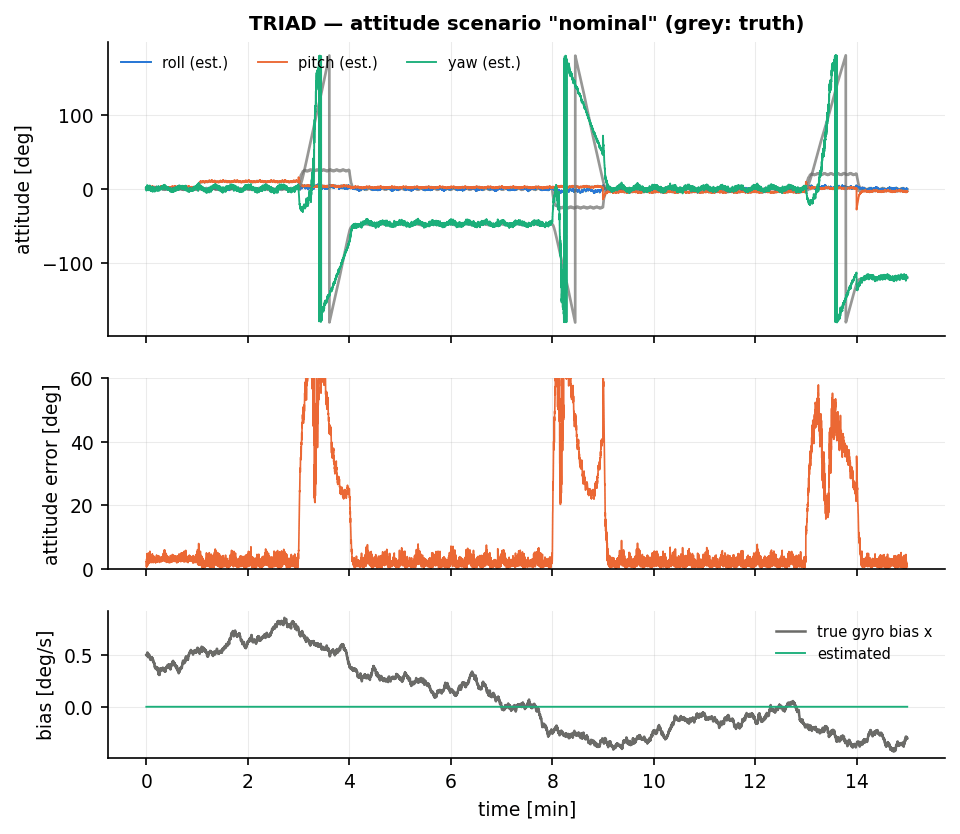
\includegraphics[width=\textwidth]{figures/imu_TRIAD_nominal.png}
\caption{TRIAD on the nominal mission. The three coordinated turns are visible as
$\SI{45}{\degree}$ error plateaus; between them the estimate tracks truth to a few degrees with no
filtering at all.}
\end{figure}
\begin{figure}[H]\centering
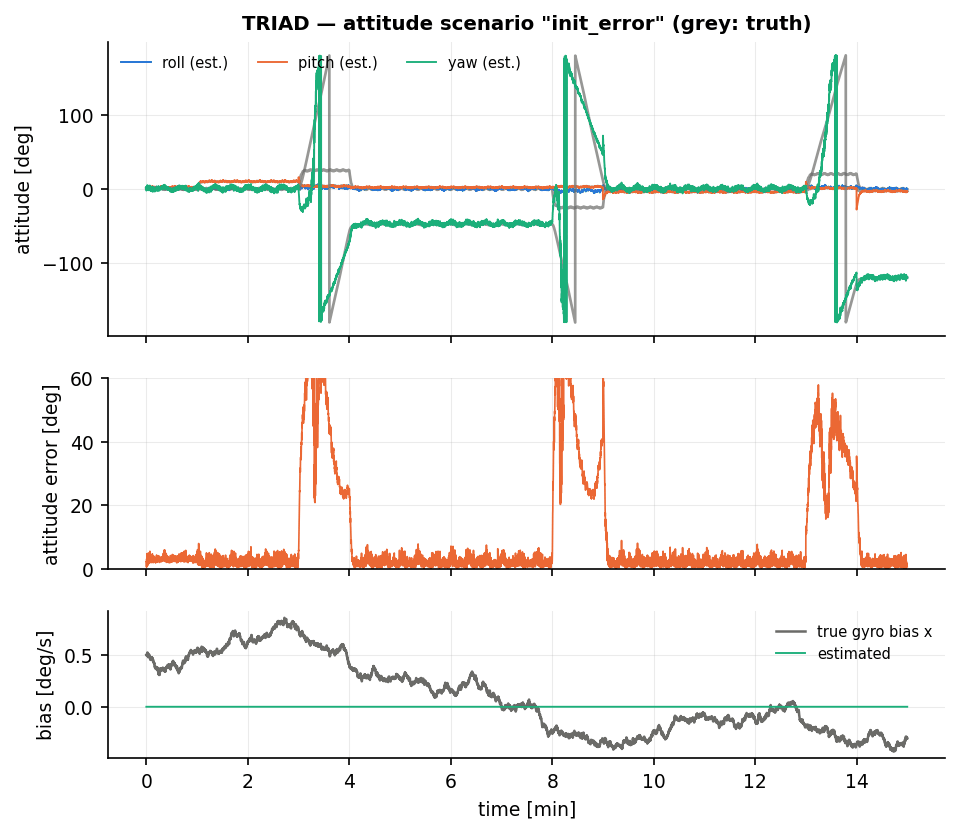
\includegraphics[width=\textwidth]{figures/imu_TRIAD_init_error.png}
\caption{TRIAD with a $46.6^\circ$ initial error --- which it does not see, being memory-less: the
trace is identical to the nominal one.}
\end{figure}

\paragraph{Insensitivity to initialisation and to the gyroscope.} \texttt{nominal},
\texttt{init\_error} and \texttt{gyro\_bias} give \emph{identical} results,
$\text{RMS}=\SI{19.59}{\degree}$, because the estimate depends on neither the initial condition nor
the gyroscope. Starting from $90^\circ$ of attitude error, TRIAD is inside $5^\circ$ at the first
sample. That is the memory-less method's one genuine advantage, and it is the reason every
practical AHRS uses it for coarse alignment: it cannot be wrong for longer than one sample because
of something that happened earlier. (Its \emph{bias} RMSE column simply reports the true bias
magnitude, $1.03$ and $\SI{3.80}{\degree\per\second}$, since it estimates none.)

\paragraph{Accelerated flight: the quantification.} Per phase on \texttt{nominal} (seed~1),
\[
3.13\;/\;2.59\;/\;\mathbf{45.21}\;/\;2.55\;/\;\mathbf{43.30}\;/\;2.51\;/\;\mathbf{36.40}\;/\;2.08
\ \SI{}{\degree}
\]
for take-off / climb / turn\,1 / cruise / turn\,2 / descent / turn\,3 / final; mission RMS
$\SI{19.59}{\degree}$, $\text{RMS}_{\text{ss}}=\SI{21.60}{\degree}$, peak $\SI{88.2}{\degree}$. In
unaccelerated flight TRIAD is a $\SI{2.5}{\degree}$--$\SI{3.1}{\degree}$ device --- within
$\SI{1.5}{\degree}$ of the six-state MEKF in the same phases
($1.30/1.50/1.74/1.91/\SI{1.86}{\degree}$), at $1/16$ of the cost --- and during the three
$\SI{60}{\second}$ coordinated turns it is a $\SI{36}{\degree}$--$\SI{45}{\degree}$ device. The
mechanism has two stages, and both are amplifications:
\begin{enumerate}[nosep]
\item In a coordinated turn the specific force lies along the body $z$ axis, so the primary
observation is wrong by the full bank angle, $\approx25^\circ$ at $t=\SI{488}{\second}$ (measured:
$\bm{f}=[-0.55,-0.81,-10.20]^\T$ against a true bank of $-24.75^\circ$). TRIAD satisfies the primary
\emph{exactly}, so this error enters the answer undiminished.
\item The magnetic field at $I=65^\circ$ has a vertical component of $\SI{43.5}{\micro\tesla}$
against $\SI{20.3}{\micro\tesla}$ horizontal. A tilt error therefore leaks into the heading with
gain $\tan I=2.14$: the $25^\circ$ tilt error becomes $\approx50^\circ$ of heading error, which is
why the yaw RMS ($\SI{17.17}{\degree}$) is nearly twice the roll RMS ($\SI{9.37}{\degree}$).
\end{enumerate}
Note that recalibrating the compass (the dataset's residual hard iron is now
$\SI{0.42}{\micro\tesla}$, a $\SI{0.65}{\degree}$ heading floor) improved the level-flight phases by
about $\SI{1.4}{\degree}$ but left the mission RMS essentially unchanged: the turns dominate, and
they are an accelerometer problem, not a magnetometer problem.

\paragraph{The collinearity degeneracy.} On \texttt{vibration} the mission RMS rises to
$\SI{27.26}{\degree}$ and the peak reaches $179.7^\circ$; $986$ of the $9\times10^4$ samples
($1.1\,\%$) exceed $90^\circ$ of error. This is \eqref{eq:tr-amplify} firing. At
$t=\SI{488.17}{\second}$ --- inside the second turn, at $-24.75^\circ$ of bank --- the measured
directions are $\bm{f}=[-0.55,-0.81,-10.20]^\T$ and $\bm{m}=[2.05,0.51,47.69]^\T$, i.e.
$\gamma=176.1^\circ$ apart, so $\norm{\bm{b}_1\times\bm{b}_2}=0.069$ and the amplification in
\eqref{eq:tr-amplify} is $1/0.069=14.5$. The reference pair is $155^\circ$ apart, so the
observations are also grossly inconsistent, and the triad construction returns an essentially
arbitrary rotation about $\bm{b}_1$. This is the practical meaning of the observability condition
$\bm{M}\succ0$ of Chapter~\ref{ch:att-mahony}, \eqref{eq:mh-lin}: two-vector attitude determination
degrades as $1/\sin\gamma$, and a steep turn at high magnetic dip drives $\gamma$ towards $\pi$.

\paragraph{The primary-sensor choice.} Making the \emph{magnetometer} primary improves the mission
RMS from $19.59$ to $\SI{18.52}{\degree}$ and the vibration case from $27.20$ to
$\SI{25.83}{\degree}$, and it redistributes the error (roll $9.37\to6.67$, pitch
$1.45\to\SI{3.74}{\degree}$). On this mission the magnetometer --- now well calibrated --- is the
more trustworthy of the two sensors, because the accelerometer is wrong by $25^\circ$ for a fifth of
the flight. That the ``obvious'' choice is the wrong one is the strongest argument for the weighted
solution of the next chapter, which does not have to choose at all.

\paragraph{Other scenarios.} \texttt{mag\_disturbance} costs $\SI{1.4}{\degree}$ ($20.97$): the
$\SI{25}{\micro\tesla}$ anomaly enters the secondary observation, attenuated by $1/\sin\gamma$,
and there is no mechanism to reject it. \texttt{high\_dynamics} costs $\SI{1.4}{\degree}$ ($20.98$,
peak $139^\circ$). The convergence metric is $-1$ and the \texttt{lost} flag is set on every
scenario --- the harness's $45^\circ$ threshold is exceeded in every turn by construction, which is
a correct description of the estimator, not a numerical failure.

\section{Summary}
TRIAD is two cross products and an orthogonalisation, 120\,bytes,
$\SI{0.13}{\micro\second}$/step, no tuning, and an answer that is independent of everything that
happened before the current sample. Use it for coarse alignment, for initialising a filter, and as
the honest lower bound on what instantaneous sensor data can deliver: in unaccelerated flight it
comes within $\SI{1.5}{\degree}$ of a six-state Kalman filter. Do not use it as an AHRS on a manoeuvring vehicle --- it satisfies the
accelerometer exactly, which is the worst possible policy when the accelerometer is the disturbed
sensor --- and be aware that its conditioning degrades as $1/\sin\gamma$ with the angle between the
two observations, which at $65^\circ$ of magnetic dip and $25^\circ$ of bank reaches
$\gamma=176^\circ$ --- close enough to $\pi$ to produce $180^\circ$ outliers in $1\,\%$ of the
samples of the \texttt{vibration} run.

% Copyright 2026 Sreeram Anil
% SPDX-License-Identifier: CC-BY-4.0
% =============================================================================
%  QUEST — Wahba's problem, Davenport's q-method, attitude (AHRS) family
% =============================================================================
\chapter{Quaternion Estimator for Wahba's Problem (QUEST)}
\label{ch:att-quest}

\section*{At a glance}
\begin{tabular}{@{}l>{\raggedright\arraybackslash}p{0.76\textwidth}@{}}
Family & attitude / AHRS (memory-less baseline) \\
Header & \texttt{include/estkit/attitude/triad\_quest.hpp} \\
Registered name & \texttt{QUEST} \\
State & none: $\bm{q}_k$ is a function of $(\bm{f}_k,\bm{m}_k)$ alone \\
Cost per step & $\approx250$ flops, $\le8$ Newton steps;
  $\SI{214}{\nano\second}$/step, 120\,bytes \\
Primary references & \cite{wahba1965,shusteroh1981,markleymortari2000,keat1977} \\
\end{tabular}

\section{Motivation and aerospace relevance}
TRIAD (Chapter~\ref{ch:att-triad}) resolves the inconsistency between two vector observations by
declaring one of them exact. Wahba~\cite{wahba1965} asked the obvious follow-up question in 1965:
what is the \emph{least-squares} attitude, weighting each observation by its accuracy and using all
of them? Her one-paragraph problem statement generated a forty-year literature; QUEST, the
``QUaternion ESTimator'' of Shuster and Oh~\cite{shusteroh1981}, is the solution that flew --- on
MAGSAT, and on most spacecraft since --- because it replaces an eigen-decomposition with a
scalar Newton iteration and a $3\times3$ matrix polynomial.

Three reasons to include it in an AHRS benchmark. It is the \emph{optimal} single-frame estimator,
so it bounds what any memory-less method can do. Its weights come directly from the sensor noise
model, so it adapts to a change in sensor quality without retuning --- the \texttt{vibration}
scenario below is exactly that experiment. And the matrix $\bm{K}$ it builds is the same object that
appears in the observability analysis of the recursive filters: the conditioning of $\bm{K}$ is why
Chapter~\ref{ch:att-mahony}'s $\bm{M}$ must be positive definite.

\section{Problem statement and assumptions}
Given $m$ pairs of unit vectors $(\bm{b}_i,\bm{r}_i)$ in the BODY and NAV frames with weights
$a_i>0$, $\sum_i a_i=1$, Wahba's problem is
\begin{equation}
\min_{\bm{A}\in SO(3)}\; L(\bm{A}) = \tfrac12\sum_{i=1}^{m} a_i\norm{\bm{b}_i-\bm{A}\bm{r}_i}^2,
\qquad \bm{A}=\bm{R}^\T\ \ (\text{NAV}\to\text{BODY}).
\label{eq:qu-wahba}
\end{equation}
Expanding and using $\norm{\bm{b}_i}=\norm{\bm{r}_i}=1$, $L(\bm{A})=\sum_i a_i - g(\bm{A})$ with the
\emph{gain function}
\begin{equation}
g(\bm{A}) = \sum_i a_i\,\bm{b}_i^\T\bm{A}\bm{r}_i = \sum_i a_i\,\bm{r}_i^\T\bm{R}\bm{b}_i ,
\label{eq:qu-gain}
\end{equation}
so minimising $L$ is maximising $g$. The maximum-likelihood interpretation
(Shuster \& Oh~\cite{shusteroh1981}, Sec.~II): if $\bm{b}_i$ is $\bm{A}\bm{r}_i$ perturbed by an
isotropic tangential error of standard deviation $\sigma_i$ radians, then \eqref{eq:qu-wahba} is the
negative log-likelihood with
\begin{equation}
a_i = \frac{\sigma_{\text{tot}}^2}{\sigma_i^2},\qquad
\sigma_{\text{tot}}^{-2}=\sum_j\sigma_j^{-2},
\label{eq:qu-weights}
\end{equation}
and QUEST is the maximum-likelihood estimator, not merely a least-squares one.

\section{Derivation}

\subsection{Davenport's \texorpdfstring{$\bm{K}$}{K} matrix}
Write the Hamilton quaternion $\bm{q}=[w,\bm{v}]$ (scalar first) for the BODY$\to$NAV rotation, so
\begin{equation}
\bm{R}(\bm{q}) = \big(w^2-\norm{\bm{v}}^2\big)\bm{I} + 2\bm{v}\bm{v}^\T + 2w[\bm{v}]_\times .
\label{eq:qu-Rq}
\end{equation}
Substituting \eqref{eq:qu-Rq} into \eqref{eq:qu-gain} and using
$\bm{r}^\T[\bm{v}]_\times\bm{b}=\bm{v}^\T(\bm{b}\times\bm{r})$ term by term,
\begin{equation}
g(\bm{q}) = \sum_i a_i\Big[(w^2-\norm{\bm{v}}^2)(\bm{r}_i\!\cdot\!\bm{b}_i)
 + 2(\bm{r}_i\!\cdot\!\bm{v})(\bm{v}\!\cdot\!\bm{b}_i)
 + 2w\,\bm{v}^\T(\bm{b}_i\times\bm{r}_i)\Big]
 = \bm{q}^\T\bm{K}\bm{q} ,
\label{eq:qu-quad}
\end{equation}
with, collecting the three groups of terms,
\begin{equation}
\bm{B}=\sum_i a_i\,\bm{b}_i\bm{r}_i^\T,\quad
\sigma=\tr\bm{B},\quad
\bm{S}=\bm{B}+\bm{B}^\T,\quad
\bm{Z}=\sum_i a_i\,(\bm{b}_i\times\bm{r}_i),\quad
\bm{K}=\begin{bmatrix}\sigma & \bm{Z}^\T\\ \bm{Z} & \bm{S}-\sigma\bm{I}\end{bmatrix}\in\real^{4\times4}.
\label{eq:qu-K}
\end{equation}
(The three checks: the $w^2$ coefficient is $\tr(\sum a_i\bm{b}_i\bm{r}_i^\T)=\sigma$; the $2w\bm{v}$
coefficient is $\bm{Z}$; and $2\bm{v}^\T\bm{B}^\T\bm{v}=\bm{v}^\T\bm{S}\bm{v}$ by symmetry.)
Equation~\eqref{eq:qu-K} is written directly for the BODY$\to$NAV Hamilton quaternion used
throughout this family, so no transposition or convention change is needed afterwards --- a
frequent source of sign errors when transcribing Shuster's vector-first, NAV$\to$BODY formulation.

$\bm{K}$ is real symmetric, so it has four real eigenvalues, and
$\max_{\norm{\bm{q}}=1}\bm{q}^\T\bm{K}\bm{q}=\lambda_{\max}$ attained at the corresponding
eigenvector. This is Davenport's $q$-method~\cite{keat1977}: \emph{the optimal quaternion is the
eigenvector of $\bm{K}$ for its largest eigenvalue}. It is exact, it never has a singularity, and it
generalises to any number of observations; the singular-value formulation of
Markley~\cite{markley1988} is the numerically most robust way to evaluate it when $m$ is large.

\subsection{QUEST: \texorpdfstring{$\lambda_{\max}$}{lambda-max} without an eigensolver}
Since $L=\sum_i a_i-\lambda_{\max}$ and the loss is small when the observations are consistent,
$\lambda_{\max}$ is close to $\sum_i a_i = 1$. Shuster and Oh therefore compute it as a root of the
characteristic polynomial, starting from $\lambda_0=\sum_i a_i$. Expanding
$\det(\bm{K}-\lambda\bm{I})$ for the structured $\bm{K}$ of \eqref{eq:qu-K} gives
(\cite{shusteroh1981}, Eq.~(63))
\begin{equation}
\lambda^4-(\alpha_a+\alpha_b)\lambda^2-\alpha_c\lambda+(\alpha_a\alpha_b+\alpha_c\sigma-\alpha_d)=0,
\label{eq:qu-char}
\end{equation}
with
\begin{align}
\kappa&=\tr(\operatorname{adj}\bm{S})=\tfrac12\big((\tr\bm{S})^2-\tr(\bm{S}^2)\big),
&\Delta&=\det\bm{S},\nonumber\\
\alpha_a&=\sigma^2-\kappa, &\alpha_b&=\sigma^2+\bm{Z}^\T\bm{Z},\label{eq:qu-abcd}\\
\alpha_c&=\Delta+\bm{Z}^\T\bm{S}\bm{Z}, &\alpha_d&=\bm{Z}^\T\bm{S}^2\bm{Z}.\nonumber
\end{align}
Newton's method on \eqref{eq:qu-char} converges quadratically from $\lambda_0$; for two
well-conditioned observations one or two iterations suffice.

\subsection{The eigenvector in closed form}
The lower block row of $\bm{K}\bm{q}=\lambda\bm{q}$ with $\bm{q}=[w,\bm{v}]$ reads
$\bm{Z}w=\big((\lambda+\sigma)\bm{I}-\bm{S}\big)\bm{v}$, i.e. with
$\bm{Y}=(\lambda+\sigma)\bm{I}-\bm{S}$,
\begin{equation}
\bm{v}=\bm{Y}\inv\bm{Z}\,w = \frac{\operatorname{adj}(\bm{Y})\bm{Z}}{\det\bm{Y}}\,w .
\label{eq:qu-eig}
\end{equation}
Choosing the (unnormalised) scale $w=\det\bm{Y}$ removes the division entirely. Expanding both
factors with the Cayley--Hamilton identity
$\operatorname{adj}\bm{Y}=\bm{Y}^2-\tr(\bm{Y})\bm{Y}+\tfrac12((\tr\bm{Y})^2-\tr\bm{Y}^2)\bm{I}$ and
$\tr\bm{S}=2\sigma$ gives, after cancellation,
\begin{align}
\alpha&=\lambda^2-\sigma^2+\kappa, &\beta&=\lambda-\sigma, \nonumber\\
\operatorname{adj}\bm{Y}&=\bm{S}^2+\beta\bm{S}+\alpha\bm{I}, &
\det\bm{Y}&=(\lambda+\sigma)\alpha-\Delta =: \gamma,
\label{eq:qu-adj}
\end{align}
so that the optimal quaternion is, in scalar-first BODY$\to$NAV form,
\begin{equation}
\bm{X}=\big(\alpha\bm{I}+\beta\bm{S}+\bm{S}^2\big)\bm{Z},
\qquad
\bm{q}_{\text{opt}} = \frac{1}{\sqrt{\gamma^2+\norm{\bm{X}}^2}}\begin{bmatrix}\gamma\\ \bm{X}\end{bmatrix}.
\label{eq:qu-q}
\end{equation}
This is Shuster and Oh's Eqs.~(66)--(72). Note that \eqref{eq:qu-q} never forms the Gibbs vector
$\bm{X}/\gamma$, which is the singular object in the original derivation: $\gamma=0$ corresponds to
a $180^\circ$ rotation and occurs twice in this mission's yaw profile, but it is harmless here,
because $\bm{X}$ is computed independently of $\gamma$ and the pair $[\gamma,\bm{X}]$ is simply
normalised. The classical ``method of sequential rotations'' is therefore unnecessary in this form.

\paragraph{Degenerate fall-back.}\label{sec:qu-fallback} The formula does fail if $\gamma$ and $\bm{X}$ vanish
\emph{together}, i.e. if $\operatorname{adj}(\bm{Y})\bm{Z}=\bm{0}$ and $\det\bm{Y}=0$. The
implementation detects this by testing $\norm{[\gamma,\bm{X}]}$ and falls back to two steps of
inverse iteration on $\bm{K}-(\lambda+\epsilon)\bm{I}$ (a $4\times4$ LU solve from
\code{linalg.hpp}), seeded with the previous estimate. It has never triggered on this benchmark, but
it costs nothing when it does not.

\subsection{TRIAD as a limit}
With $m=2$ and $a_1\to1$, $a_2\to0$, the maximiser of \eqref{eq:qu-gain} must satisfy
$\bm{R}\bm{b}_1=\bm{r}_1$ exactly and then maximise the residual term --- which is the TRIAD
construction. Shuster and Oh~\cite[Sec.~IV]{shusteroh1981} make this precise: for two observations,
TRIAD is QUEST with an infinite weight ratio, so the two differ only through
\eqref{eq:qu-weights}.

\section{Algorithm}
\begin{algorithm}[H]
\caption{QUEST --- one sampling period (the gyroscope is ignored)}
\begin{algorithmic}[1]
\Require $\bm{f},\bm{m}$; references $\bm{r}_1,\bm{r}_2$; weights $a_1,a_2$ from \eqref{eq:qu-weights}
\State $\bm{b}_1\gets\bm{f}/\norm{\bm{f}}$;\; $\bm{b}_2\gets\bm{m}/\norm{\bm{m}}$
\State $\bm{B}\gets a_1\bm{b}_1\bm{r}_1^\T+a_2\bm{b}_2\bm{r}_2^\T$;\; $\sigma\gets\tr\bm{B}$;\;
       $\bm{S}\gets\bm{B}+\bm{B}^\T$;\; $\bm{Z}\gets a_1\bm{b}_1\times\bm{r}_1+a_2\bm{b}_2\times\bm{r}_2$
\State $\kappa\gets\tfrac12((\tr\bm{S})^2-\tr\bm{S}^2)$;\; $\Delta\gets\det\bm{S}$;\;
       $(\alpha_a,\alpha_b,\alpha_c,\alpha_d)\gets$ \eqref{eq:qu-abcd}
\State $\lambda\gets a_1+a_2$
\For{$j=1,\dots,J$} \Comment{Newton on \eqref{eq:qu-char}, $J=8$}
  \State $\lambda\gets\lambda-\dfrac{\lambda^4-(\alpha_a+\alpha_b)\lambda^2-\alpha_c\lambda+(\alpha_a\alpha_b+\alpha_c\sigma-\alpha_d)}{4\lambda^3-2(\alpha_a+\alpha_b)\lambda-\alpha_c}$;\;
        \textbf{break if} converged
\EndFor
\State $\alpha\gets\lambda^2-\sigma^2+\kappa$;\; $\beta\gets\lambda-\sigma$;\;
       $\gamma\gets(\lambda+\sigma)\alpha-\Delta$;\;
       $\bm{X}\gets(\alpha\bm{I}+\beta\bm{S}+\bm{S}^2)\bm{Z}$
\State \textbf{if} $\norm{[\gamma,\bm{X}]}$ negligible \textbf{then} inverse iteration on $\bm{K}$
\State $\bm{q}_k\gets[\gamma,\bm{X}]/\norm{[\gamma,\bm{X}]}$
\Ensure $\bm{q}_k$
\end{algorithmic}
\end{algorithm}

\section{Application to the benchmark flight}
The weights are derived from the configured sensor noise through \eqref{eq:qu-weights}: the
direction error of a vector measurement of magnitude $\norm{\bm{v}}$ with per-axis noise $\sigma$ is
$\sigma/\norm{\bm{v}}$ radians, so $\sigma_1=\sigma_a/g$ and $\sigma_2=\sigma_m/B$. On the nominal
scenario this gives
\begin{equation}
\sigma_1=\frac{0.05}{9.807}=\SI{5.1e-3}{\radian},\quad
\sigma_2=\frac{0.5}{48}=\SI{10.4e-3}{\radian}
\;\Longrightarrow\;
a_1=0.807,\ a_2=0.193 ,
\label{eq:qu-wnom}
\end{equation}
and on \texttt{vibration}, where the harness raises the configured accelerometer noise to
$\SI{1.05}{\metre\per\second\squared}$, $\sigma_1=\SI{107e-3}{\radian}$ and the weights become
$a_1=0.009$, $a_2=0.991$: the estimator hands the problem to the magnetometer \emph{without being
retuned}. No other estimator in this family adapts to the configuration this directly, and the
benchmark measures the consequence below.

Eight Newton iterations are allowed with a relative break at $10^{-12}$; in practice one or two are
executed.

\section{Implementation notes}
Per step: two outer products and two cross products ($\approx24$ MACs), $\bm{S}^2$ (27),
$\det\bm{S}$ (9 explicit, not via LU), three quadratic forms in $\bm{Z}$ ($\approx30$), the Newton
loop ($\approx10$ flops per iteration) and the $3\times3$ polynomial in \eqref{eq:qu-q} ($\approx30$):
about 250 flops with a single \code{sqrt} beyond the measurement normalisations. Measured
$\SI{214}{\nano\second}$/step, about $66\,\%$ more than TRIAD and still under a quarter of a
microsecond; \code{sizeof} is 120\,bytes, identical to TRIAD because the two share a class and
neither stores anything beyond the last quaternion and the weights.

Numerical hygiene: $\det\bm{S}$ is expanded in closed form rather than by LU, so there is no
pivoting and no failure branch; the Newton loop breaks if $\abs{f'}<10^{-12}$ and is bounded by
$J=8$; \eqref{eq:qu-q} is guarded by a finiteness and magnitude test with the inverse-iteration
fall-back described above; the step is skipped entirely if either measurement magnitude is below
$10^{-6}$. No NaN or infinity was produced on any of the six scenarios
($1.6\times10^{6}$ samples over three seeds). The single-precision build reproduces the
double-precision mission RMS to four digits.

The limitation is structural and shared with TRIAD: no state, no gyroscope, no memory. QUEST is the
best possible \emph{instantaneous} answer, which on a manoeuvring aircraft is not a good answer.

\section{Benchmark results}
% Copyright 2026 Sreeram Anil
% SPDX-License-Identifier: CC-BY-4.0
\begin{table}[H]\centering\footnotesize\setlength{\tabcolsep}{3.5pt}\caption{QUEST: attitude benchmark (mean over seeds; all angles in degrees; $t_\mathrm{conv}$: first time the attitude error stays below 2$^\circ$ for 30\,s; bias RMSE in deg/s; 120 bytes of state).}\label{tab:imu_QUEST}
\begin{tabular}{lrrrrrrrrcr}\toprule scenario & RMS & roll & pitch & yaw & max & RMS$_\mathrm{ss}$ & $t_\mathrm{conv}$ [s] & bias RMSE & lost & ns/step \\ \midrule
nominal & 19.22 & 8.68 & 1.44 & 17.18 & 87.7 & 21.18 & -- & 1.03 & yes & 214 \\
init\_error & 19.22 & 8.68 & 1.44 & 17.18 & 87.7 & 21.18 & -- & 1.03 & yes & 213 \\
gyro\_bias & 19.22 & 8.68 & 1.44 & 17.18 & 87.7 & 21.18 & -- & 3.80 & yes & 215 \\
mag\_disturbance & 20.63 & 8.69 & 1.44 & 18.73 & 87.7 & 21.18 & -- & 1.03 & yes & 215 \\
vibration & 25.89 & 9.10 & 4.93 & 24.28 & 179.7 & 27.94 & -- & 1.03 & yes & 225 \\
high\_dynamics & 20.63 & 9.12 & 1.54 & 18.57 & 138.8 & 22.60 & -- & 1.03 & yes & 216 \\
\bottomrule\end{tabular}\end{table}

\begin{figure}[H]\centering
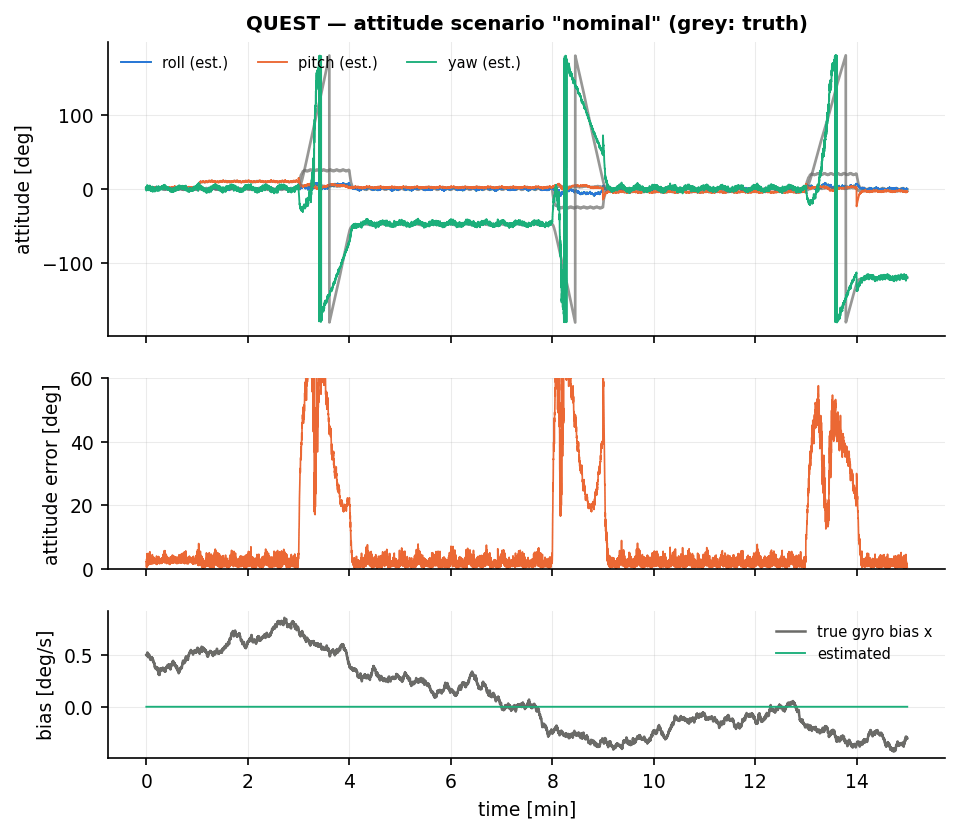
\includegraphics[width=\textwidth]{figures/imu_QUEST_nominal.png}
\caption{QUEST on the nominal mission: the optimal single-frame solution, which during the
coordinated turns is optimally wrong.}
\end{figure}
\begin{figure}[H]\centering
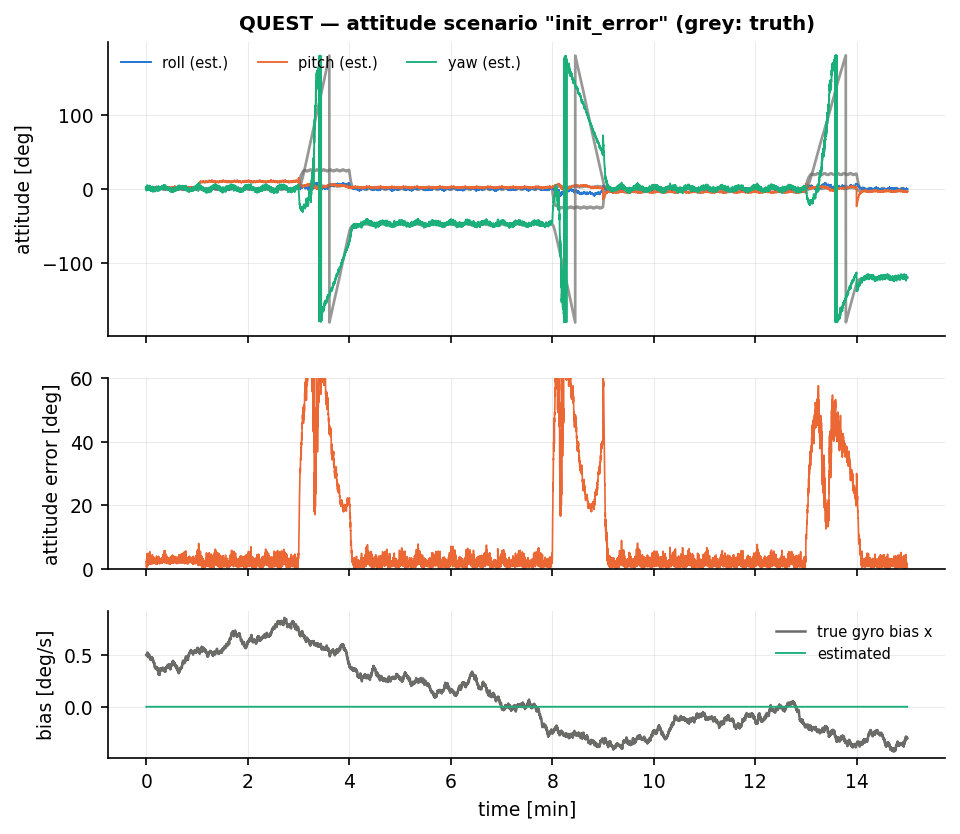
\includegraphics[width=\textwidth]{figures/imu_QUEST_init_error.png}
\caption{QUEST with a $46.6^\circ$ initial error, which it ignores: the trace is identical to the
nominal one.}
\end{figure}

On \texttt{nominal} QUEST gives $\text{RMS}=\SI{19.22}{\degree}$ (roll $8.68$, pitch $1.44$, yaw
$\SI{17.18}{\degree}$), $\text{RMS}_{\text{ss}}=\SI{21.18}{\degree}$, peak $\SI{87.7}{\degree}$ and
$\SI{214}{\nano\second}$/step at 120\,bytes. Like TRIAD it returns \emph{identical} numbers on
\texttt{init\_error} and on \texttt{gyro\_bias}, since it uses neither the initial condition nor
the gyroscope, and its bias RMSE column simply reports the true bias magnitude ($1.03$ and
$\SI{3.80}{\degree\per\second}$). Per phase (seed~1),
\[
2.76\;/\;2.58\;/\;\mathbf{44.42}\;/\;2.52\;/\;\mathbf{42.32}\;/\;2.50\;/\;\mathbf{35.86}\;/\;2.04
\ \SI{}{\degree}
\]
for take-off / climb / turn\,1 / cruise / turn\,2 / descent / turn\,3 / final. The interpretation is
the one given in Chapter~\ref{ch:att-triad} and needs no repetition: in unaccelerated flight the
instantaneous solution is a $\SI{2.5}{\degree}$ device --- close to what the sensors themselves
permit --- while during the three coordinated turns the accelerometer reports zero bank and the
$65^\circ$ magnetic dip amplifies the resulting tilt error into the heading by $\tan I=2.14$.

Table numbers are three-seed means; the variants below are single-seed (seed~1) diagnostics.

\paragraph{QUEST versus TRIAD.} Optimal weighting buys $\SI{0.37}{\degree}$ on \texttt{nominal}
($19.22$ against $\SI{19.59}{\degree}$) and redistributes the error sensibly (roll $8.68$ against
$9.37$). That is a small return, and the reason is \eqref{eq:qu-wnom}: at $a_1=0.807$ the optimal
solution is already close to the accelerometer-primary TRIAD limit, so the two nearly coincide. It
buys more where the weights are far from that limit: on \texttt{vibration} QUEST gives
$\SI{25.89}{\degree}$ against TRIAD's $\SI{27.26}{\degree}$, its pitch RMS is $4.93$ against $6.23$,
and its outlier count is $964$ samples above $90^\circ$ against TRIAD's $986$. This is the
\emph{adaptivity} experiment: the configured accelerometer noise rises by a factor of 21, the
weights swing from $(0.81,0.19)$ to $(0.01,0.99)$ automatically, and the estimator degrades by
$\SI{6.7}{\degree}$ instead of $\SI{7.7}{\degree}$. Forcing equal weights $a_1=a_2=0.5$ gives
$\SI{18.79}{\degree}$ on nominal but $\SI{26.18}{\degree}$ on vibration --- better on the scenario it
happens to suit, worse where the weighting matters, which is the usual fate of a fixed tuning.

\paragraph{The Newton iteration earns its place.} Truncating the iteration degrades the result
measurably: $J=8$ (registered) gives $\SI{19.23}{\degree}$, $J=1$ gives $\SI{20.05}{\degree}$, and
$J=0$ --- i.e. the common approximation $\lambda_{\max}\approx\sum_i a_i$, exact only for consistent
observations --- gives $\SI{24.32}{\degree}$ with a peak of $179.9^\circ$. On this mission the
observations are grossly inconsistent for a fifth of the flight, so $\sum_i a_i$ is a poor estimate
of $\lambda_{\max}$ and the closed form \eqref{eq:qu-q} evaluated at the wrong $\lambda$ is not even
a rotation-optimal answer. Two iterations recover essentially all of it, and the degenerate
fall-back of \S\ref{sec:qu-fallback} never triggered.

\paragraph{The collinearity degeneracy.} Like TRIAD, QUEST produces large outliers on
\texttt{vibration}: $964$ of $9\times10^4$ samples ($1.1\,\%$) exceed $90^\circ$, and the peak is
$179.8^\circ$. The cause is the conditioning of $\bm{K}$, not of the algorithm: at
$t=\SI{488.17}{\second}$, in a $-24.75^\circ$ banked turn, the measured directions are $176.1^\circ$
apart while the references are $155^\circ$ apart, so $\bm{S}-\sigma\bm{I}$ is nearly rank-deficient
in the plane containing both and the maximiser of \eqref{eq:qu-quad} is nearly degenerate. No
weighting can repair an observation geometry in which the two measured directions are almost
anti-parallel; only a gyroscope can, which is the entire argument for the filters in the rest of
this family.

\paragraph{Other scenarios.} \texttt{mag\_disturbance} costs $\SI{1.4}{\degree}$ ($20.63$), entirely
in yaw ($17.18\to\SI{18.73}{\degree}$) as expected for a horizontal field offset;
\texttt{high\_dynamics} costs $\SI{1.4}{\degree}$ ($20.63$, peak $138.8^\circ$). Both scenarios set
the \texttt{lost} flag and neither converges under the harness's $2^\circ$-for-$\SI{30}{\second}$
criterion --- correct descriptions of a memory-less estimator on this mission, not numerical
failures.

\section{Summary}
QUEST is the optimal single-frame attitude estimator: maximum likelihood under isotropic tangential
noise, closed form, $\SI{0.21}{\micro\second}$/step, 120\,bytes, and weights that follow the sensor
noise model with no tuning. Use it for coarse alignment, for initialising a recursive filter, for
star-tracker-style problems where the observations really are simultaneous and independent, and as
the honest optimum against which any memory-less claim must be measured. On this mission it beats
TRIAD by $\SI{0.37}{\degree}$ in nominal conditions and by $\SI{1.4}{\degree}$ under vibration ---
the payoff of weighting is largest exactly when the sensors differ most --- but both remain
$\SI{17}{\degree}$ behind the six-state filters and $\SI{17}{\degree}$ behind a
$\SI{132}{\nano\second}$ gated Mahony observer, because the missing ingredient is not a better
algebraic solution, it is the time axis.

